\documentclass[specialist,
               substylefile = spbu.rtx,
               subf,href,colorlinks=true, 12p]{disser}

\usepackage[a4paper,
            mag=1000, includefoot,
            left=3cm, right=1.5cm, top=2cm, bottom=2cm, headsep=1cm, footskip=1cm]{geometry}
\usepackage[T2A]{fontenc}
\usepackage[utf8]{inputenc}
\usepackage[english,russian]{babel}
\ifpdf\usepackage{epstopdf}\fi
\usepackage{amssymb,amsfonts,amsmath,amsthm}
\usepackage{bm}
\usepackage{float}
\usepackage{amsmath}
\usepackage{caption}
\usepackage{hyperref}
\usepackage{cleveref}
\usepackage{booktabs}
\usepackage{multirow}
\usepackage{graphicx}
\usepackage{pdflscape}
\usepackage{longtable}


\DeclareMathOperator{\SSA}{SSA}
\DeclareMathOperator{\diag}{diag}
\DeclareMathOperator{\MSE}{MSE}
\DeclareMathOperator{\RMSE}{RMSE}
\newcommand{\multiref}[2]{\ref{#1}---\ref{#2}}

% Точка с запятой в качестве разделителя между номерами цитирований
%\setcitestyle{semicolon}

% Использовать полужирное начертание для векторов
\let\vec=\mathbf

% Включать подсекции в оглавление
\setcounter{tocdepth}{1}

\graphicspath{{fig/}}

%----------------------------------------------------------------
\begin{document}

%
% Титульный лист на русском языке
%
% Название организации
\institution{%
	Санкт-Петербургский государственный университет
}

\title{Выпускная квалификационная работа}

% Тема
\topic{Использование метода SSA в машинном обучении для прогноза временных рядов}

% Автор
\author{\textsc{Ежов} Федор Валерьевич}
%\group{группа 20.М03-мм}
\group{%
	Уровень образования: магистратура\\
	Направление 01.04.02 <<Прикладная математика и информатика>>\\
	Основная образовательная программа ВМ.5751.2020 <<Математическое моделирование, программирование и искусственный интеллект>>
}

% Научный руководитель
\sa       {Н.\,Э.~Голяндина}
\sastatus {Доцент, кафедра статистического моделирования\,\\
	к.ф.-м.н., доцент}

% Рецензент
\rev      {А.\,Ю.~Шлемов}
\revstatus{Программист, Майкрософт Израиль}

% Город и год
\city{Санкт-Петербург}
\date{\number\year}

\maketitle

%%
%% Titlepage in English
%%
%
\institution{%
	Saint Petersburg State University \\
	Applied Mathematics and Computer Science \\
	Statistical Modelling
}
%
\title{Graduation Project}
%
%% Topic
\topic{On using the SSA method in machine learning to predict time series}
%
%% Author
\author{\textsc{Ezhov} Fedor} % Full Name
\group{}

%% Scientific Advisor
\sa       {N.~Golyandina}
\sastatus {Associate Professor, Department of Statistical Modelling}
%
%% Reviewer
\rev      {А.~Shlemov}
\revstatus{Software developer, Microsoft R\&D, Israel}
%
%% City & Year
\city{Saint Petersburg}
\date{\number\year}

\maketitle[en]

\tableofcontents

\chapter*{Введение}
\addcontentsline{toc}{chapter}{Введение}
Методы машинного обучения, в частности, нейронные сети используются для решения многих задач анализа данных. Чтобы улучшить результаты, нередко применяют процедуры предобработки данных. В данной работе решается задача прогнозирования временного ряда с помощью нейронных сетей. 
Мы будем рассматривать модель временного ряда в виде зашумленного детерминированного сигнала. В этом случае логично использовать предобработку временного ряда, которая выделяет сигнал или, как минимум, снижает уровень шума. В качестве метода для такой предобработки был выбран метод Singular Spectrum Analysis (SSA) \cite{SSA}. Данный метод может хорошо выделить большой класс сигналов, а также прогнозировать временной ряд. С появлением методов, использующих предобработку SSA, так называемых гибридных методов, возникает желание сравнить их с негибридными аналогами. Целью работы является разработка методологии сравнения обычных и гибридных методов, а также прогноза методом SSA в задаче прогнозирования временных рядов.

Исследованиями влияния обработки SSA для нейронных сетей занимались и ранее, например можно посмотреть статьи \cite{wang2015daily, wu2010prediction, Wu2011}. Первоначальная мотивация данной работы была получена из статьи \cite{ar1}. В статье рассматривалось сравнение нейронной сети MultiLayer Perceptron (MLP) (в работах и далее именуемая как ANN, как она называлась в \cite{ar1}) и ее гибридного аналога с предобработкой SSA на реальных данных <<Indian Rain>>. Авторы той статьи утверждали, что предобработка портит точность прогноза, а предыдущие статьи, показывающие преимущество гибридных методов, не учитывали возникающий так называемый <<data leaking>> (когда метод получает информацию, к которой не должен иметь доступ, например из будущего). В данной работе мы постараемся опровергнуть утверждение из \cite{ar1} и продемонстрировать обратный эффект; особое внимание будет уделено построении схемы без <<data leaking>>. К ANN и SSA-ANN добавим рекуррентные нейронные сети Recurrent neural network (RNN) \cite{rnn}, Gated Recurrent Unit (GRU) \cite{gru}, Long short-term memory (LSTM) \cite{lstm}, а также их гибридные аналоги SSA-RNN, SSA-GRU, SSA-LSTM. 

Кроме данных <<Indian Rain>> рассмотрим также данные Earth \linebreak orientation parameters (EOP), прогнозируемые в статье \cite{eopart}, где метод SSA показывал хорошие результаты. 
%В этой работе также было сравнение проведено обычных и гибридных методов, а также метода SSA на данных EOP. К удивлению, гибридные методы не показали такого улучшения в точности прогноза, как на данных <<Indian Rain>>. Метод SSA показал лучшую точность.

Также рассмотрим данные характеристики погоды в Санкт-Петербурге (данные были взять с площадки для соревнований Kaggle).
%На этих данных не удалось получить существенного улучшения результатов гибридными методами.

Так как одной из целей является понять, почему результаты сравнения гибридных и негибридных методом те или иные, рассмотрим также модельные ряды, а именно сумму синусов с белым шумом и сумму синусов с красным шумом. На модельных данных исследуем эффекты влияние наличия шума на точность прогнозирования, влияние размера ряда, влияние выбора параметров в метода SSA, а также влияния на результат прогноза красного шума в данных.

Для того чтобы результаты сравнения были убедительными и устойчивыми, в работе предлагается методика сравнения методов. Методика учитывает зависимость ошибки прогноза от параметров нейронных сетей, выбор наилучших параметров SSA для гибридных методов, отображение результатов прогнозов, отображение выделенного сигнала с помощью метода SSA, проверку устойчивости результатов.

Структура работы следующая. В главах \ref{chapter_SSA} и \ref{models} описаны обе составляющие методов прогноза --- алгоритм Singular Spectrum Analysis (SSA) и нейронные сети, соответственно. В главе \ref{chapterSSAML} показано, каким образом строятся гибридные методы, а также в разделе \ref{comp_tactic} предлагается методика сравнения гибридных и негибридных методов, используемая далее. Применению этой методики посвящены главы \ref{modts} и \ref{chapter_realdata}. В главе \ref{modts} описаны эксперименты на модельных данных. В главе \ref{chapter_realdata} описаны эксперименты на реальных данных. Заключение коротко резюмирует результаты. Так как методика включает в себя большое количество графических изображений результатов, часть из вынесена в приложение.

\chapter{Алгоритм Singular Spectrum Analysis}
\label{chapter_SSA}
Метод SSA используется для разложение исходного ряда в сумму рядов, которые легко интерпретировать и понять их поведение. Обычно исходный ряд раскладывается в сумму трех рядов: тренд --- медленно меняющаяся компонента, сезонность --- циклическая компонента с фиксированным периодом и шум. Информацию про базовый алгоритм SSA и связанные с методом фундаментальные понятия можно найти в книге <<Analysis of time series structure: SSA and related techniques>> \cite{SSA}.

Алгоритм SSA состоит из четырех этапов:
\begin{enumerate}
	\item Построение траекторной матрицы (Вложение).
	\item SVD.
	\item Группировка первых $r$ собственных троек.
	\item Диагональное усреднение.
\end{enumerate}

Рассмотрим каждый этап подробнее. Пусть $\mathsf{X}_N = (x_1, \ldots, x_{N})$ --- временной ряд, где $N > 3$. Также будем предполагать, что найдется хоть одно $x_i \neq 0$, то есть ряд не нулевой. Обычно считается, что $x_i = f(i\Delta)$ для некоторой функции $f(t)$, где $t$ --- время, а $\Delta$ --- некоторый временной интервал. \\

\section{Этап 1. Построение траекторной матрицы (Вложение)}
Выберем целое $L$ --- длина окна, такое что $1 < L < N$. Тогда $K = N - L - 1$.
Построим вектора
$X_i = (x_{i} , \dots, x_{i+L-1})^\mathrm{T}$, для $1 \leqslant i \leqslant K$.
Составим из векторов $X_i$ траекторную матрицу:

$$\mathbf{X} = [X_1 : \cdots : X_K] =
\begin{pmatrix}
	x_1& x_2& x_3& \cdots& x_{K} \\
	x_2& x_3& x_4& \cdots& x_{K+1} \\
	x_3& x_4& x_5& \cdots& x_{K+2} \\
	\vdots& \vdots& \vdots& \ddots& \vdots \\
	x_{L}& x_{L+1}& x_{L+2}& \cdots& x_{N}
\end{pmatrix}
.$$

Получили матрицу $\mathbf{X}$ размерностью $L \times K$, составленную из пересекающихся частей  исходного временного ряда. Можно заметить, что на побочных диагоналях стоят одинаковые числа, такая матрица называется ганкелевой. Существует взаимно-однозначное соответствие между ганкелевыми матрицами $L \times K$ и рядами длиной $N = L + K - 1$.

Операцию получения из ряда $\mathsf{X}_N$ траекторную матрицу $\mathbf{X}$ обозначим:
$$ \mathbf{X} = \mathcal{T}_L(\mathsf{X}_N), $$
обратную операцию обозначим, как $\mathcal{T}^{-1}$ соответственно.

\section{Этап 2. Singular Value Decomposition (SVD)}
\label{ssasvd}
На данном этапе применяется метод SVD к траекторной матрице $\mathbf{X}$. Пусть $ \mathbf{S}  = \mathbf{X}\mathbf{X}^\mathrm{T}$ и $\lambda_1 > \dotsc > \lambda_L$ --- собственные числа матрицы $\mathbf{S}$, $U_1, \dotsc, U_L$ --- ортонормированная система базисных векторов, соответствующих собственным числам. Обозначим $V_i = \dfrac{X^\mathrm{T} U_i}{\sqrt \lambda_i}$ и $d = max\{i : \lambda_i > 0\}$. Тогда сингулярное разложение матрицы $\mathbf{X}$ запишется следующим образом:

$$\mathbf{X} = \mathbf{X}_1 + \dotsc + \mathbf{X}_d \text{, где } \mathbf{X}_i = \sqrt \lambda_i U V^\mathrm{T}, $$

Набор $(\sqrt \lambda_i, U_i, V^\mathrm{T}_i)$ будем называть i-й собственной тройкой.

\section{Этап 3. Группировка первых $r$ собственных троек}
На этапе группировки из всех значений $\{1 \dotsc d\}$ берутся первые $r$. Пусть, $I = \{1, \dotsc , r\}$, тогда результирующая матрица соответствующая группе $I$ имеет вид:
$\mathbf{X}_{I} = \mathbf{X}_{1} + \dotsc + \mathbf{X}_{r}$.

\section{Этап 4. Диагональное усреднение}
Пусть $\mathbf{Y}$ --- матрица $L \times K$ и $ L < K$. $y_{ij}$ - элементы матрицы, где $1 \leqslant i \leqslant L, 1 \leqslant j \leqslant K$,  $N = L + K - 1$.  Диагональное усреднение преобразует матрицу $\mathbf{Y}$ в ряд $g_0, \dotsc , g_{N-1}$ по формуле:

\begin{equation*}
	g_k =
	\begin{cases}
		\dfrac{1}{k+1} \sum \limits_{m=1}^{k+1} y_{m, k-m+2} &  \text{, для } 0 \leqslant k < L-1,\\
		\dfrac{1}{L} \sum \limits_{m=1}^L y_{m, k-m+2} &  \text{, для } L-1 \leqslant k < K,\\
		\dfrac{1}{N-k} \sum \limits_{m=k-K+2}^{N-K+1} y_{m, k-m+2} & \text{, для } K \leqslant k < N.
	\end{cases}
\end{equation*}

Применяя диагональное усреднение к результирующей матрице группы $I$, получаем ряд $\widehat{\mathsf{F}} = (\hat{f}_1, \ldots, \hat{f}_{N-1})$. Ряд $\widehat{\mathsf{F}}$ назовем оценкой сигнала, полученной с помощью SSA.
Процедуру выделения сигнала с помощью SSA обозначим как:
$$ \widehat{\mathsf{F}} = \SSA_{L, r}(\mathsf{F}), $$
где $L$ --- длина окна в SSA, $r$ --- количество первых собственных троек, участвующие в построении $\widehat{\mathsf{F}}$.

\chapter{Архитектуры нейронных сетей}
\label{models}
В данной главе рассматриваются нейронные сети используемые в работе. Всего рассмотрено четыре архитектуры: одна линейная (называемая ANN), и три рекуррентных нейронных сети --- RNN, LSTM, GRU.

Каждая нейронная сеть имеет параметры и гиперпараметры. Параметры, или по-другому веса, оптимизируются на тренировочной выборке в процессе обучения. Гиперпараметры --- это переменные, задаваемые пользователем, например количество скрытых слоев, их размеры и т.~д. Они выбираются на основе некоторых суждений или перебором ориентируюсь на точность, сосчитанную на валидационной выборке. Архитектура или модель нейронной сети определяется с точностью до гиперпараметров. Термин модель означает конкретный нейросетевой метод (например ANN или LSTM), не стоит путать его с моделью временного ряда. Нейронные сети оптимизируют (подгоняют) параметры для решения задачи прогнозирования сигнала ряда во время процесса <<обучения>>. Процессом обучения называется оптимизация параметров нейронной сети с помощью градиентного метода <<обратного распространения ошибки>> или его модификаций. В данной работе нейронные сети <<обучаются с учителем>>, то есть на парах <<признаки --- предсказываемые значения>>.


\section{Artificial Neural Network (ANN)}

Artificial Neural Network (ANN) включает в себя входной слой, ряд скрытых слоев и выходной слой, каждый слой содержит несколько узлов. Теорема Цыбенко гласит, что ANN с одним скрытым слоем может аппроксимировать любую непрерывную функцию многих переменных с любой точностью. Поэтому далее в этой работе, будем рассматривать ANN с одним скрытым слоем. ANN формализуется следующим образом:

Входные данные, на которых модель учиться делать предсказания:
$$ X = (x_1, \ldots, x_T).$$
Предсказания модели:
$$ \widehat{Y} = (\hat{y}_1, \ldots, \hat{y}_R). $$
Формула, описывающая модель:
$$ y_k = \phi_2\bigg(\sum\limits_{j=1}^{h} w^{(2)}_{jk} \phi_1(\sum\limits_{i=1}^{T} w^{(1)}_{ij} x_{i} + \theta^{(1)}_{j})  + \theta^{(2)}_k \bigg), k = [1, \ldots, R], $$
где $T$ --- размер входного вектора, на котором выполняется прогноз. $h$ --- размер скрытого слоя. $w$ и $\theta$ --- веса модели. $\phi$ --- функции активации. $R$ --- размер выходного вектора-прогноза.

Список некоторых функций активации:
\begin{enumerate}
	\item Линейная функция активации: $\phi(x) = x$.
	\item Сигмоида: $\sigma(x) = \dfrac{1}{1 + e^{-x}}$.
	\item $\mathrm{ReLU}(x) = \begin{cases}
		0, & x < 0, \\
		x, & x \geqslant 0.
	\end{cases}$
\end{enumerate}

Далее в работе рассматривается архитектура ANN с $\phi_1$ --- ReLU и $\phi_2$ --- линейной функцией активации. Выбор параметра $h$ обсуждается в следующих главах.

\section{Recurrent neural network (RNN)}

Модель recurrent neural network (RNN), использует рекурсию в своих архитектурах для решения задач, где данные содержатся в некоторой последовательности (например, временные ряды, текстовые задачи и др.). В RNN присутствует вектор скрытого слоя, служащий для <<накопления>> информации.

$X^\mathrm{T} = (x_1, \ldots, x_T)$ --- вектор входных данных.

$ J_t^\mathrm{T} = (j_1, \ldots, j_h)$ --- вектор скрытого слоя в момент $t$.

$ \widehat{Y}_T^\mathrm{T} = (\hat{y}_1, \ldots, \hat{y}_R) $ --- вектор выходных данных в момент $T$.

Следующие формулы описывают модель:
\begin{gather*}
	J_t = f_j(U x_{t} + \theta_1 + \mathbf{W} J_{t-1} + \theta_2), \\
	\widehat{Y}_T = f_y(\mathbf{V} J_T + \theta_3),
\end{gather*}
где $t = 1, \ldots, T$;  $\mathbf{V}, \mathbf{W}, U, \theta_i$ -- веса модели, которые вычисляются в процессе обучения, $f_j, f_y$ -- функции активации.

Далее в работе рассматривается архитектура RNN с $f_j$ --- гиперболический тангенс и $f_y$ --- линейной функцией активации. Выбор параметра $h$ обсуждается в следующих главах.


\section{Long short-term memory (LSTM)}

Long short-term memory (LSTM) --- разновидность рекуррентных моделей, с добавлением второго скрытого слоя, используемого для <<долгосрочной>> памяти.

$X^\mathrm{T} = (x_1, \ldots, x_T)$ --- вектор входных данных.

$ J_t^\mathrm{T} = (j_1, \ldots, j_h)$ --- вектор скрытого слоя в момент $t$.

$ C_t^\mathrm{T} = (c_1, \ldots, c_h)$ --- вектор скрытого слоя в момент $t$.

$\widehat{Y}_T^\mathrm{T} = (\hat{y}_1, \ldots, \hat{y}_R)$ --- вектор выходных данных в момент $T$.

Следующие формулы описывают модель:
\begin{gather*}
	f_t = \sigma(\mathbf{W}_f \cdot [J_{t-1}, x_t] + b_f), \,
	i_t = \sigma(\mathbf{W}_i \cdot [J_{t-1}, x_t] + b_i), \\
	\widetilde{C}_t = \tanh(\mathbf{W}_c \cdot [J_{t-1}, x_t] + b_c), \,
	C_t = f_t * C_{t_1} + i_t * \widetilde{C}_t, \\
	o_t = \sigma(\mathbf{W}_o \cdot [J_{t-1}, x_t] + b_o), \,
	J_t = o_t * \tanh(C_t), \\
	\widehat{Y}_T = f(\mathbf{V} J_T + b_0),
\end{gather*}
где $t = 1, \ldots, T$; $\mathbf{W}, \mathbf{V}, b$ --- веса модели, $\sigma(x), \tanh(x), f(x)$ --- функции активации. Оператор $*$ --- производит поэлементное умножение.

Далее в работе рассматривается архитектура LSTM с $f$ --- линейной функцией активации. Выбор параметра $h$ обсуждается в следующих главах.

\section{Gated Recurrent Unit (GRU)}

Gated Recurrent Unit (GRU) --- модель похожая на LSTM, но без дополнительного скрытого слоя.

$X^\mathrm{T} = (x_1, \ldots, x_T)$ --- вектор входных данных.

$ J_t^\mathrm{T} = (j_1, \ldots, j_h)$ --- вектор скрытого слоя в момент $t$.

$\widehat{Y}_T^\mathrm{T} = (\hat{y}_1, \ldots, \hat{y}_R) $ --- вектор выходных данных в момент $T$.

Следующие формулы описывают модель:
\begin{gather*}
	z_t = \sigma(\mathbf{W}_z \cdot [J_{t-1}, x_t] + b_z), \,
	r_t = \sigma(\mathbf{W}_r \cdot [J_{t-1}, x_t] + b_r), \\
	\widetilde{J}_t = \tanh(\mathbf{W} \cdot [r_t * J_{t-1}, x_t] + b), \,
	J_t = (1 - z_t) * J_{t-1} + z_t * \widetilde{J}_t, \\
	Y_T = f(\mathbf{V} J_T + b_0),
\end{gather*}
где $t = 1, \cdots, T$;  $\mathbf{W}, \mathbf{V}, b$ --- веса модели, $\sigma(x), \tanh(x), f(x)$ --- функции активации. Оператор $*$ --- производит поэлементное умножение.

Далее в работе рассматривается архитектура LSTM с $f$ --- линейной функцией активации. Выбор параметра $h$ обсуждается в следующих главах.

\chapter{Использование SSA в машинном обучении}
\label{chapterSSAML}
\section{Задача}
Рассмотрим $\mathsf{Z}_N$ --- временной ряд длины $N$ и задачу: с помощью модели некоторой нейронной сети $f$ на основе $T$ последовательных точек ряда $\mathsf{Z}_N$, предсказать следующие $R$ точек ряда.
$$ [\widehat{z}_{i+T+1}, \ldots , \widehat{z}_{i+T+R}] = f ([z_{i+1}, \ldots, z_{i+T}]). $$

Считаем, что $ \mathsf{Z}_N = \mathsf{S}_N + \xi_N, $ где $\mathsf{S}_N$ -- сигнал, $\xi_N$ -- шум, случайный процесс с нулевым мат. ожиданием. Тогда возникает идея, подавать на вход методу $f$ не сам ряд, а оценку сигнала $\widehat{\mathsf{S}}_N$, полученную с помощью метода SSA. Методы $f$, которым на вход подается $\widehat{\mathsf{S}}_N$ называем гибридными. Разница между обычными и гибридными методами заключается только в данных, поступающих на вход. Таким образом решение поставленной задачи, можно разбить на несколько частей: подготовка данных, обучение методов, прогнозирование.

\section{Подготовка данных}
$\mathsf{Z}_N$ --- изначальный временной ряд длиной $N$.
Можем представить ряд в виде траекторной матрицы для длины окна $T + R$:


$$ \mathbf{Z} = \mathcal{T}_{T+R}(\mathsf{Z}_N) = $$

\begin{equation*} 
	= \begin{pmatrix}
		z_1 & z_2 & \cdots & z_{T} & \vrule & z_{T+1} &  \cdots & z_{T+R-1} & z_{T+R} \\
		z_2 & z_3 & \cdots & z_{T+1} & \vrule & z_{T+2} &  \cdots & z_{T+R} & z_{T+R+1} \\
		\vdots & \vdots & \ddots & \vdots & \vrule & \vdots & \ddots & \vdots & \vdots  \\
		z_{N-T-R+1} & z_{N-T-R+2} & \cdots & z_{N-R} & \vrule & z_{N-R+1} &  \cdots & z_{N-1} & z_{N} \\
	\end{pmatrix}.
\end{equation*}

Матрица $\mathbf{Z}$ имеет размерность $(N - T - R + 1) \times (T + R)$. Левую часть матрицы $\mathbf{Z}$ обозначим $\mathbf{Z}^x$, правую --- $\mathbf{Z}^y$. Разобъем матрицу по строчкам на три части: train, val, test. Пусть $\tau$, $v$ и $t$ номера последних строчек в каждой соответствующей части.
Обозначим часть матрицы $\mathbf{Z}$ с $a$ по $b$ строчку и с $c$ по $d$ столбец как $\mathbf{Z}_{a,b}^{(c, d)}$. Тогда train, val, test записываются как: $\mathbf{Z}_{train} = \mathbf{Z}_{1,\tau}^{(1, T+R)}, \mathbf{Z}_{val} = \mathbf{Z}_{\tau+T+R,v}^{(1, T+R)}, \mathbf{Z}_{test} = \mathbf{Z}_{v+T+R,t}^{(1, T+R)}$. В этих же обозначениях $\mathbf{Z}^x = \mathbf{Z}_{1,t}^{(1, T)}, \mathbf{Z}^y = \mathbf{Z}_{1,t}^{(T+1, T+R)}$.

\subsubsection{SSA-preprocessing}
\label{SSA-preprocessing}
В этом разделе опишем алгоритм предобработки SSA для тренировочной выборки. Пусть $L, r$ --- гиперпараметры, описанные в главе \ref{chapter_SSA}.

\begin{enumerate}
	\item Преобразуем train часть матрицы $\mathbf{Z}$ во временной ряд $\widetilde{\mathsf{Z}} = \mathcal{T}^{-1}(\mathbf{Z}_{train})$.
	\item Получим ряд $\widehat{\mathsf{Z}} = SSA_{L, r}(\widetilde{\mathsf{Z}})$.
	\item Получаем траекторную матрицу $\mathbf{\widehat{Z}} = \mathcal{T}_{T + R}(\widehat{\mathsf{Z}})$. Матрица $\mathbf{\widehat{Z}}$ и будет результатом работы предобработки SSA для тренировочной выборки.
\end{enumerate}

В отличие от тренировочной выборки, о которой все известно, считается, что о валидационной и тестовой выборках нет информации. В этих случаях SSA-обработку следует применять так, чтобы предыдущие значения ряда не получали информации от будущих (<<заглядывание в будущее>>).

Пусть $\mathsf{Z}_{b, e} = [z_b, z_{b+1}, \ldots, z_e]$ подряд ряда $ \mathsf{Z} $, где $ b $ --- начальный индекс, $ e $ --- конечный индекс. Пусть $ p $ --- тоже индекс ряда, такой что $b < p < e$. Следующий алгоритм описывает процедуру получения ряда $\mathsf{Z}_{p+1, e}$, обработанного с помощью SSA без <<заглядывание в будущее>>:

\begin{enumerate}
	\item Пусть есть ряд $\mathsf{Z}_{b, e}$ и задано $p$. Тогда $Q = e - p$ --- размер ряда $ \mathsf{Z}_{p+1, e} $. Пусть $ \widehat{\mathsf{Z}}_Q = (\hat{z}_1, \ldots, \hat{z}_Q) $ --- ряд размера $Q$.
	\item Для каждого $ i = [1, \ldots, Q] $ получим: $$\widehat{\mathsf{Z}}^{'}_{b+i-1, p+i} = \mathrm{SSA}_{L, r}(\mathsf{Z}_{b+i-1, p+i}). $$
	Присвоим значение последнего элемента полученного ряда $\hat{z}^{'}_{p+i}$ значению ряда $\widehat{\mathsf{Z}}_Q$ с соответствующим индексом, $\hat{z}_i = \hat{z}^{'}_{p+i}$.
	\item Получили ряд $\widehat{\mathsf{Z}}_Q$ размера $ Q $, значения которого являются значениями ряда  $\mathsf{Z}_{p+1, e}$, обработанные с помощью SSA без <<заглядывания в будущее>>.
\end{enumerate}

Обозначим процедуру получения $\widehat{\mathsf{Z}}_Q = \mathrm{SSA}^{(p)}(\mathsf{Z}_{b, e})$. Заметим, что для предобработки валидационной и тестовой выборок логично взять $Q = \tau + T$ ($\tau + T$ --- длина ряда $\mathcal{T}^{-1}(\mathbf{Z}_{train}^x)$, который является тренировочной выборкой представленым в виде ряда). Алгоритм предобработки для валидационной выборки запишется следующим образом:

\begin{enumerate}
	\item Запишем $\mathbf{Z}_{1,v}^{(1, T+1)}$ как $\mathsf{Z}_{1, v + T + 1}$.
	\item Выберем $p = \tau + T + 1$.
	\item Получим $\widehat{\mathsf{Z}}_Q = \mathrm{SSA}^{(p)}(\mathsf{Z}_{1, v + T + 1})$.
	\item Перейдем обратно к траекторной матрице $\widehat{\mathbf{Z}}_{\mathrm{val}} = \mathcal{T}_{T+1}(\widehat{\mathsf{Z}}_Q) $, которая будет результатом предобработки SSA для валидационной выборки.
\end{enumerate}

Размерность $\widehat{\mathbf{Z}}_{\mathrm{val}}$ будет совпадать с размерностью $\mathbf{Z}_{\mathrm{val}}$. Аналогичным образом строится тестовая выборка.

\section{Обучение нейронной сети}

Оптимизация параметров нейросетевой модели проводится с помощью алгоритма <<обратного распространения ошибки>> или его модификаций на тренировочной выборке. Модель учится по строчкам $\mathbf{Z}^x_{train}$ предсказывать строчки $\mathbf{Z}^y_{train}$. Эпоха --- цикл прохода всех строчек из тренировочной выборки матрицы $\mathbf{Z}_{train}$ в процессе обучении. Валидационная выборка используется для оценки точности модели и оптимизации гиперпараметров. Переобучение по параметрам предотвращается с помощью механизма ранней остановки. Данный алгоритм останавливает обучение, если ошибка на валидационной выборке растет на протяжение некоторого количества эпох.

Перед началом обучения нужно выбрать гиперпараметры модели и количество эпох. Так как в обучении используется алгоритм ранней остановки, возьмем заведомо большое количество эпох. Более подробно выбор параметров написал в разделе \ref{comp_tactic}. Стоит уточнить, что далее в работе выбор гиперпараметров производится только для метода SSA в гибридных моделях, в других же случаях производится полный перебор по сетке параметров.

Алгоритм обучения модели после выбора архитектуры:

\begin{enumerate}
	\item Инициализация модели со случайными весами.
	\item На тренировочной выборке $\mathbf{Z}_{train}$ оптимизируются веса $w, \theta$ с заданным количеством эпох. Модель учится по данным строчкам $\mathbf{Z}^x_{train}$ предсказывать соответствующие строчки $\mathbf{Z}^y_{train}$. Для каждой $i$-ой эпохи считается $\varepsilon_i$ --- ошибка на валидационной выборке. Для валидационной выборки $\mathbf{Z}^x_{val}$ строится прогноз $\widehat{\mathbf{Z}}^y_{val}$. Ошибка $\varepsilon_i$ получается сравнением $\widehat{\mathbf{Z}}^y_{val}$ с $\mathbf{Z}^y_{val}$ по какой-нибудь метрике (например MSE).
	\item Срабатывает механизм ранней остановки. Присваиваем параметрам модели те, которые были получены при минимальной ошибке $\min(\varepsilon_i)$.
\end{enumerate}

\section{Прогнозирование}


\subsection{Прогнозирование с помощью нейронных сетей}

После того как модель обучена, можно перейти к прогнозированию точек ряда.

\begin{enumerate}
	\item Возьмем  $\mathbf{Z}^x_{test}$ и $\mathbf{Z}^y_{test}$.
	\item Представим $\mathbf{Z}^x_{test} = [Z_{test}^{x, 1} : \cdots : Z_{test}^{x, Q}]^\mathrm{T}, $ где $Q$ --- количество строчек в тестовой матрицы $ \mathbf{Z}_{test} $.
	\item Для каждой строчки матрицы $\mathbf{Z}^x_{test}$ получаем прогноз с помощью обученной модели. Запишем результат прогноза как\linebreak матрицу $ \mathbf{\widehat{Z}}^y = [\widehat{Z}^{y, 1} : \cdots : \widehat{Z}^{y, Q}]^\mathrm{T}$.
	\item Далее можно сравнить $\mathbf{\widehat{Z}}^y $ с $\mathbf{Z}^y_{test}$ по какой-нибудь метрике.
\end{enumerate}

\subsection{Прогнозирование SSA}

Рассмотрим способ линейного рекуррентного прогноза (ЛРФ) методом SSA. Будем прогнозировать на одну точку вперед, тогда формула прогноза по ЛРФ запишется следующим образом.

\begin{equation*}
	\hat{y}_{N+1} = \sum_{i = 1}^{L - 1} \alpha_k \hat{f}_{N - k + 1},
\end{equation*}
где $\hat{f}_i$ --- элементы оценки сигнала ряда, построенным с помощью метода SSA, а $\alpha_i$ --- коэффициенты ЛРФ и $\alpha_{L-1} \neq 0$.

Обозначим собственный вектора $U_i$ SVD разложения из раздела \ref{ssasvd} без последнего элемента как $\underline{U_i}$, а последний элемент --- $\pi_i$. Тогда коэффициенты ЛРФ можно получить по формуле ниже.

\begin{equation*}
	(\alpha_{L-1}, \ldots, \alpha_{1})^\mathrm{T} = \dfrac{1}{1- v^2} \sum_{i=1}^r \pi_i \underline{U_i},
\end{equation*}
где $v^2 = \sum_{i=1}^r \pi_i^2$.

\section{Метрики качества прогноза}
С помощью метрик MSE и RMSE можно измерить размер ошибки полученного прогноза.
$$ \MSE(\mathbf{Z}^y_{test}, \mathbf{\widehat{Z}}^y) = \frac{1}{Q} \diag\bigg((\mathbf{Z}^y_{test} - \mathbf{\widehat{Z}}^y) (\mathbf{Z}^y_{test} - \mathbf{\widehat{Z}}^y)^\mathrm{T}\bigg), $$
$$ \RMSE(\mathbf{Z}^y_{test}, \mathbf{\widehat{Z}}^y) = \sqrt{\MSE(\mathbf{Z}^y_{test}, \mathbf{\widehat{Z}}^y)}. $$

\section{Методика применения и сравнения методов}
\label{comp_tactic}
В этом разделе описана методика применения и сравнения обычных и гибридных прогнозов, а также прогнозов полученных с помощью SSA. Программную реализацию данной методики можно найти в \cite{Ezhov2022}.

\paragraph{Прогноз по SSA} Подберем для метода SSA параметры $L$ и $r$, которые дают наилучшие результаты на валидационной выборке. Для параметров $L$ и $r$ зададим сетку, по которой будем перебирать комбинации параметров, оценивая ошибку прогноза на один шаг вперед с помощью метрики RMSE на валидационной выборке. Построим график с кривыми зависимости ошибки от параметра $L$. Каждая кривая будет соответствовать одному параметру $r$ из соответствующей сетки.

Далее, для пяти лучших пар параметров построим прогноз на тестовой выборке и получим оценку ошибки. Каждую ошибку отобразим на графике с помощью горизонтальной прямой вместе с прогнозами обычных и гибридных методов.

\paragraph{Выбор параметров SSA в гибридных моделях} Прежде чем сравнивать обычные и гибридные модели, нужно выбрать параметры SSA для гибридных моделей. Сделать это можно двумя способами:

\begin{enumerate}
	\item Подобрать параметры на основе SSA-анализа тренировочной части ряда.
% или исходя из других источников информации.
	\item Перебрать параметры для метода SSA и выбрать лучшие параметры, основываясь на точности прогноза методом, полученной на предыдущем этапе.
\end{enumerate}

\paragraph{Обычные и гибридные методы} Для гибридных моделей фиксируем параметры SSA $L$ и $r$, выбранные заранее. Будем сравнивать методы по сетке гиперпараметров $T$ --- размер входного вектора и $h$ --- размер скрытого слоя нейронной сети (модели нейронных сетей подробно описаны в главе \ref{models}). Каждую пару $T$ и $h$ можно представить как ячейку в таблице \ref{hyperP_grid}. Для каждой ячейки получаем ошибку по метрике RMSE на тестовой выборке. Ошибку можно усреднить по столбцам или по строкам, и построить по графику зависимости ошибки от гиперпараметров $T$ или $h$ для каждого метода соответственно. Методы можно будет сравнить на графиках.

\begin{table}[h]
\caption{Сетка гиперпараметров.}
\begin{center}
		\begin{tabular}{l|l|l|l|l|}
		\cline{2-5}
		& \multicolumn{1}{c|}{$T_1$} & \multicolumn{1}{c|}{$T_2$} & \multicolumn{1}{c|}{$\cdots$} & \multicolumn{1}{c|}{$T_n$} \\ \hline
		\multicolumn{1}{|l|}{$h_1$}    & $(T_1, h_1)$               & $(T_2, h_1)$               & $\cdots$                      & $(T_n, h_1)$               \\ \hline
		\multicolumn{1}{|l|}{$h_2$}    & $(T_1, h_2)$               & $(T_2, h_2)$               & $\cdots$                      & $(T_n, h_2)$               \\ \hline
		\multicolumn{1}{|l|}{$\vdots$} & $\vdots$                   & $\vdots$                   & $\ddots$                      & $\vdots$                   \\ \hline
		\multicolumn{1}{|l|}{$h_m$}    & $(T_1, h_m)$               & $(T_2, h_m)$               & $\cdots$                      & $(T_n, h_m)$               \\ \hline
	\end{tabular}
\end{center}
\label{hyperP_grid}
\end{table}

Заметим, что для модельных данных, где сигнал известен, можно также использовать данные сигнала для анализа ошибок методов.

\paragraph{Проверка устойчивости результатов}
Для того чтобы оценить устойчивость результатов, фиксируется небольшая сетка параметров $T$ и строится таблица, аналогичная \ref{hyperP_grid}. Проводится $n$ реализаций для каждой ячейки из таблицы. Так как параметры в нейронных сетях инициализируется случайно, то каждый раз получается разный результат. Для каждого $T$ полученные результаты заносятся на отдельный график зависимости ошибки от параметра $h$ в виде точек. По этим графикам можно оценить устойчивость результатов.

\paragraph{Отображение прогнозов} Чтобы объяснить успешность или неуспешность прогноза и в целом посмотреть на картину прогнозирования, будем строить график прогноза на один шаг на тестовых данных на фоне правильных ответов.

\paragraph{Восстановление ряда с помощью SSA} Для оценки корректности использования предобработки SSA будем строить график восстановленного сигнала с помощью SSA на фоне временного ряда (его тренировочной части).

\paragraph{Таблица с результатами}
Для каждого примера вместе с графиками сравнения будет приводиться таблица с числовыми результатами, которые строятся на основе таблиц с суммарными результатами \ref{bigtable}, \ref{real_bigtable}. Общие таблицы \ref{bigtable}, \ref{real_bigtable} объединяет результаты, полученные для всех примеров для модельных или реальных данных соотвественно. Опишем сначала общую таблицу.
В столбце <<ssa-params>> отображены параметры SSA в гибридных моделях, если параметры не указаны, значит в строчке записаны результаты для негибридных моделей. Префикс <<b>> значит, что значение в таблице отображает ошибку лучшей нейронная сеть (например, лучшая из ANN, или лучшая из гибридной SSA-ANN с указанными параметрами SSA). Префикс <<m>> означает, что значение отображает среднее значение ошибок для соответствующих негибридных, обычных методов или метода SSA. При этом для методов с использование нейронных сетей при вычислении общего среднего по методу откидывались наименьшее и наибольшее среднее по $T$ в таблице \ref {hyperP_grid} из средних при разных $h$. Для метода SSA показана наименьшее значение ошибки для префикса <<b>>, для префикса <<m>> показано среднее значение по пяти лучшим прогнозом, при этом для удобства сравнения во всех строчках ошибки SSA-прогноза повторены.

% Префикс <<b>> значит, что значение в таблице отображает наименьщую ошибку метода из его семейства (например, лучшая из ANN, или лучшая из гибридной SSA-RNN с указанными параметрами SSA, или лучшая прогноз SSA).

В отдельных таблицах для каждого примеры префикс <<b>> значит, что значение в таблице отображает ошибку лучшей нейронная сеть из своих аналогов (например, лучшая из негибридных, или лучшая из гибридных с указанными параметрами SSA). Префикс <<m>> означает, что значение отображает среднее значение ошибок для негибридных, обычных методов или метода SSA, где среднее считается по значениям из таблицы \ref{bigtable}. Для метода SSA значения повторены из таблицы \ref{bigtable}.

В целом, интерес для анализа представляют значения из столбцов с префиксов <<m>>, а лучшие значения показаны просто для информации, так как результат не является устойчивым.

\chapter{Модельные данные}
\label{modts}

В данной главе на модельных рядах проведены эксперименты с целью показать влияние различных особенностей временных рядов и способов выбора параметров методов на результаты точности прогнозов и на результаты сравнения методов прогноза. В главе рассмотрено:

\begin{enumerate}
	\item Влияние выбора параметра $r$.
	\item Влияние величины шума во временном ряде.
	\item Влияние красного шума во временном ряде.
\end{enumerate}

\section{Сумма двух синусов с белым шумом}
\label{edsine}

Рассмотрим следующий ряд, состоящий из элементов: $$ z_i = \big(\sin(2 \pi \dfrac{i}{6} ) + 2 \cdot \sin(2 \pi \dfrac{i}{12} ) \big) + \kappa \varepsilon_i, $$ где $\varepsilon_i \in \mathrm{N}(0, 1)$, $\kappa$ задает размер шума в ряде. Так как сигнал ряда состоит из двух синусов, его ранг равен $4$. Обозначим $\mathsf{X}_N$ ряд с $\kappa = 0.3$, а $\mathsf{Z}_N$ с $\kappa = 1.5$. Далее в этом разделе рассматриваем ряды: $\mathsf{X}_{650}, \; \mathsf{Z}_{650}, \; \mathsf{Z}_{1500}$. На рис. \ref{edsine_graph} представлен ряд $\mathsf{Z}_{650}$.

В экспериментах будем разбивать ряды длиной ${650}$ на тренировочную, валидационную, тестовую выборки по $350$, $150$, $150$ точек соответственно. А ряд длиной ${1500}$ --- по $750$, $500$, $250$ точек соответственно.

В данном ряде легко оценить сигнал, это можно увидеть на периодограмме (рис. \ref{edsine_pgram}). Шум в ряде не очень большой, хотя видно что он присутствует. В данном примере сигнал стоит из двух синусов с периодами $12$ и $6$, общий период ряда $12$. Далее в экспериментах будем перебирать параметры $T$ и $L$ по сетке с шагом кратным $12$. Будем считать аналитически верными параметрами для этого ряда $L = 175$ (половина длины тренировочной выборки) и $r = 4$, так как ранг ряда равен $4$, а $L = 175$ удовлетворяет условию асимптотической разделимости.

\begin{figure}[H]
	\captionsetup{justification=centering}
	\center{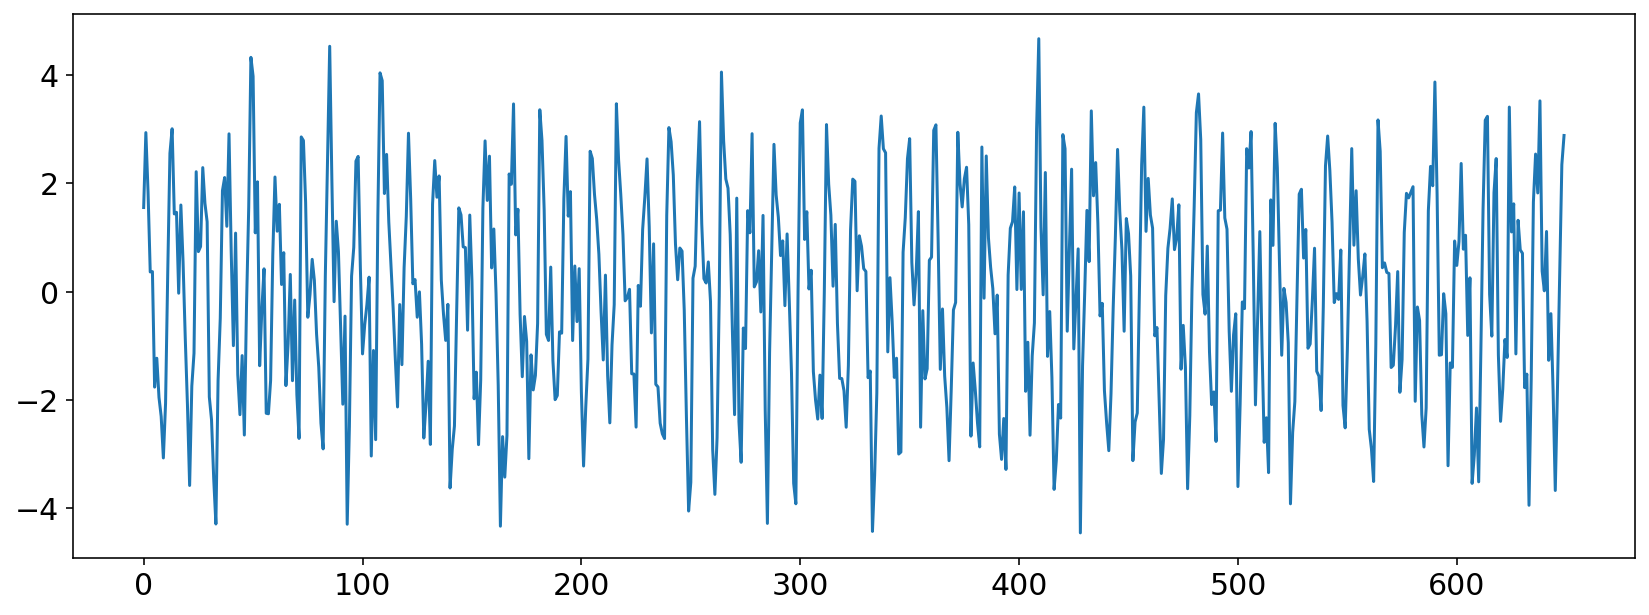
\includegraphics[width=0.9\linewidth]{imgs/ts/edsine/edsine_graph}}
	\caption{Ряд <<сумма синусов с белым шумом>>, $\mathsf{Z}_{650}$.}
	\label{edsine_graph}
\end{figure}

\begin{figure}[H]
	\captionsetup{justification=centering}
	\center{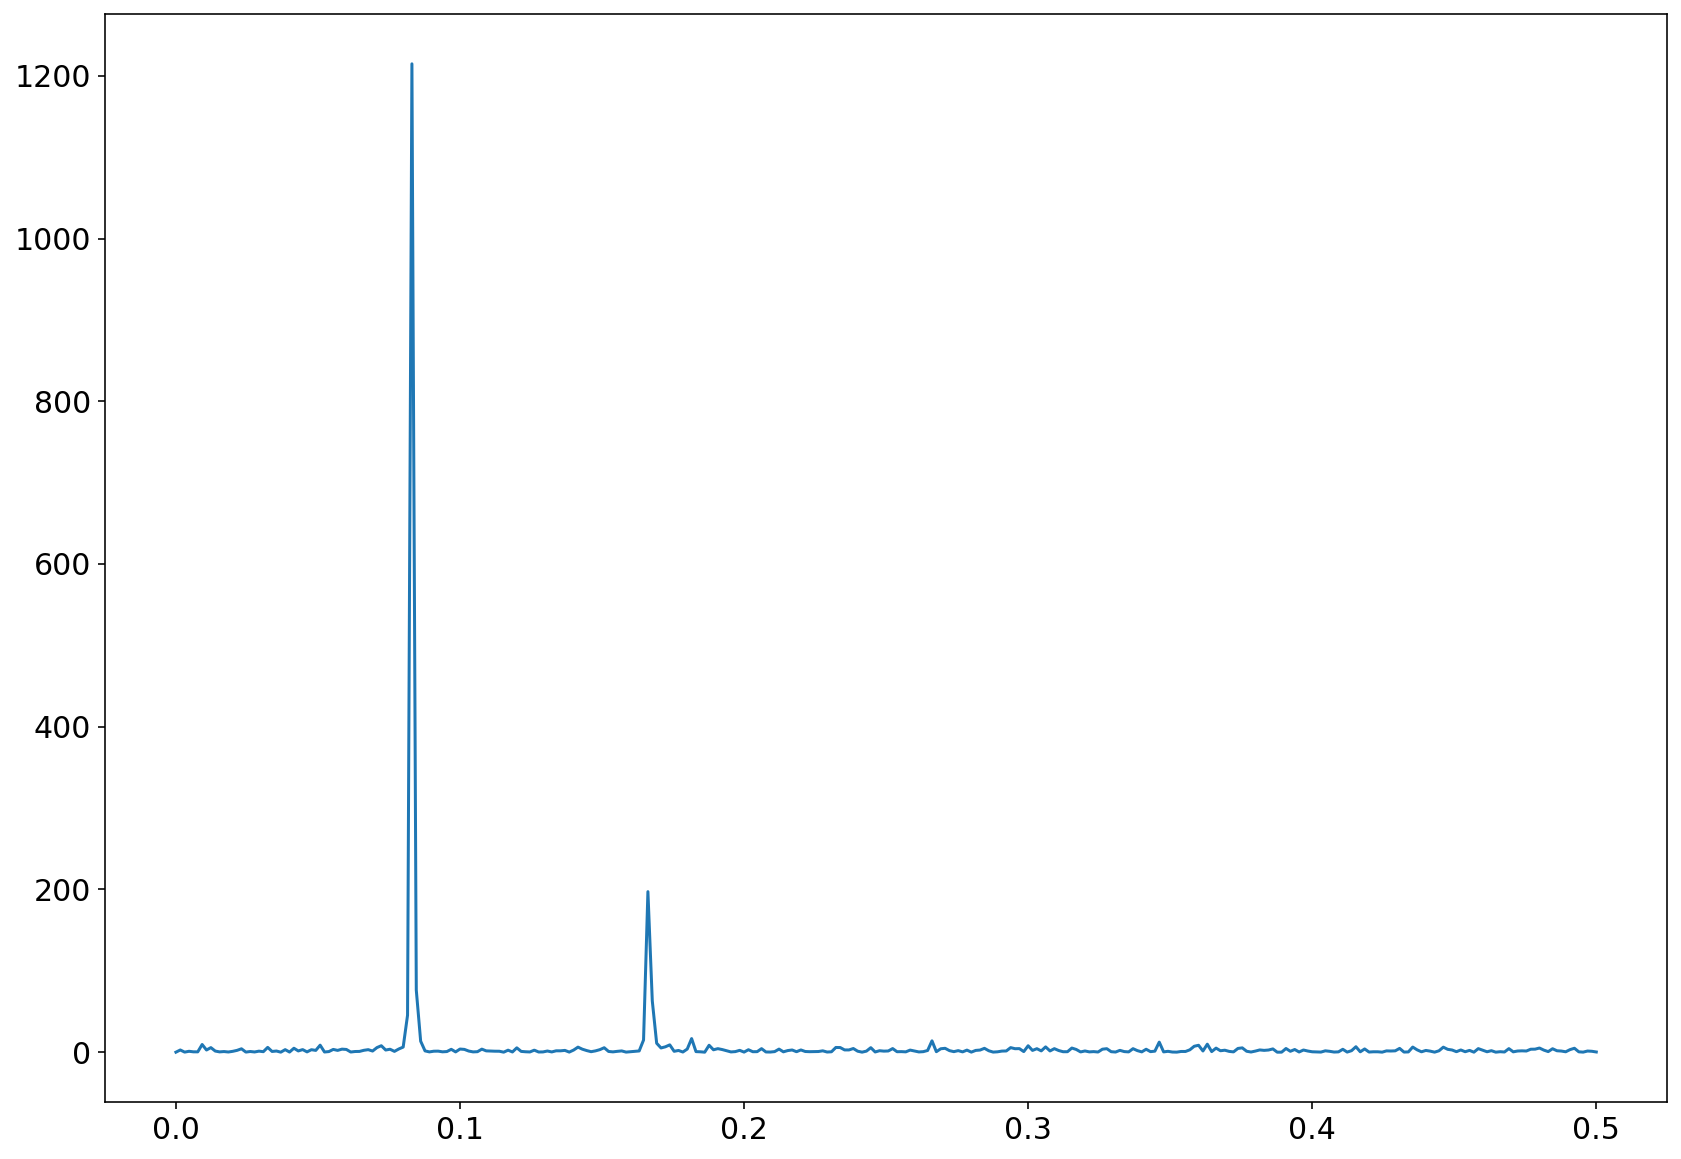
\includegraphics[width=0.9\linewidth]{imgs/ts/edsine/edsine_pgram}}
	\caption{Периодограмма ряда <<сумма синусов с белым шумом>>, $\mathsf{Z}_{650}$.}
	\label{edsine_pgram}
\end{figure}

\subsection{Влияние выбора параметра $r$}
\label{edsinr}
Поставим задачу сравнить обычные и гибридные методы при разных выбранных значениях параметра $r$ в гибридных методах. Будем проводить сравнение на ряде $\mathsf{Z}_{650}$. Далее будем работать с тремя различными параметрами: правильно выбранное $r = 4$, недостаточно большое $r = 2$, слишком большое $r = 6$. Каждый вариант будем исследовать с помощью методологии, описанной в разделе \ref{comp_tactic}.

В тексте работы будем приводить только часть рисунков, а полный анализ можно найти в приложении к работе.

\subsubsection{Прогноз по SSA}

Сравним точность прогнозирования методом SSA при разных параметрах $r$ на валидационном периоде. Зададим следующую сетку параметров $L = \{12, 24, \ldots, 175\}$, $r = \{2, 4, 6\}$. Посмотрим на результаты на рисунке \ref{edsinr_ssa_forecast}. На графике видно, что наилучшие результаты достигаются при $r = 4$, худшие результаты достигаются при $r = 6$.

\begin{figure}[H]
	\captionsetup{justification=centering}
	\center{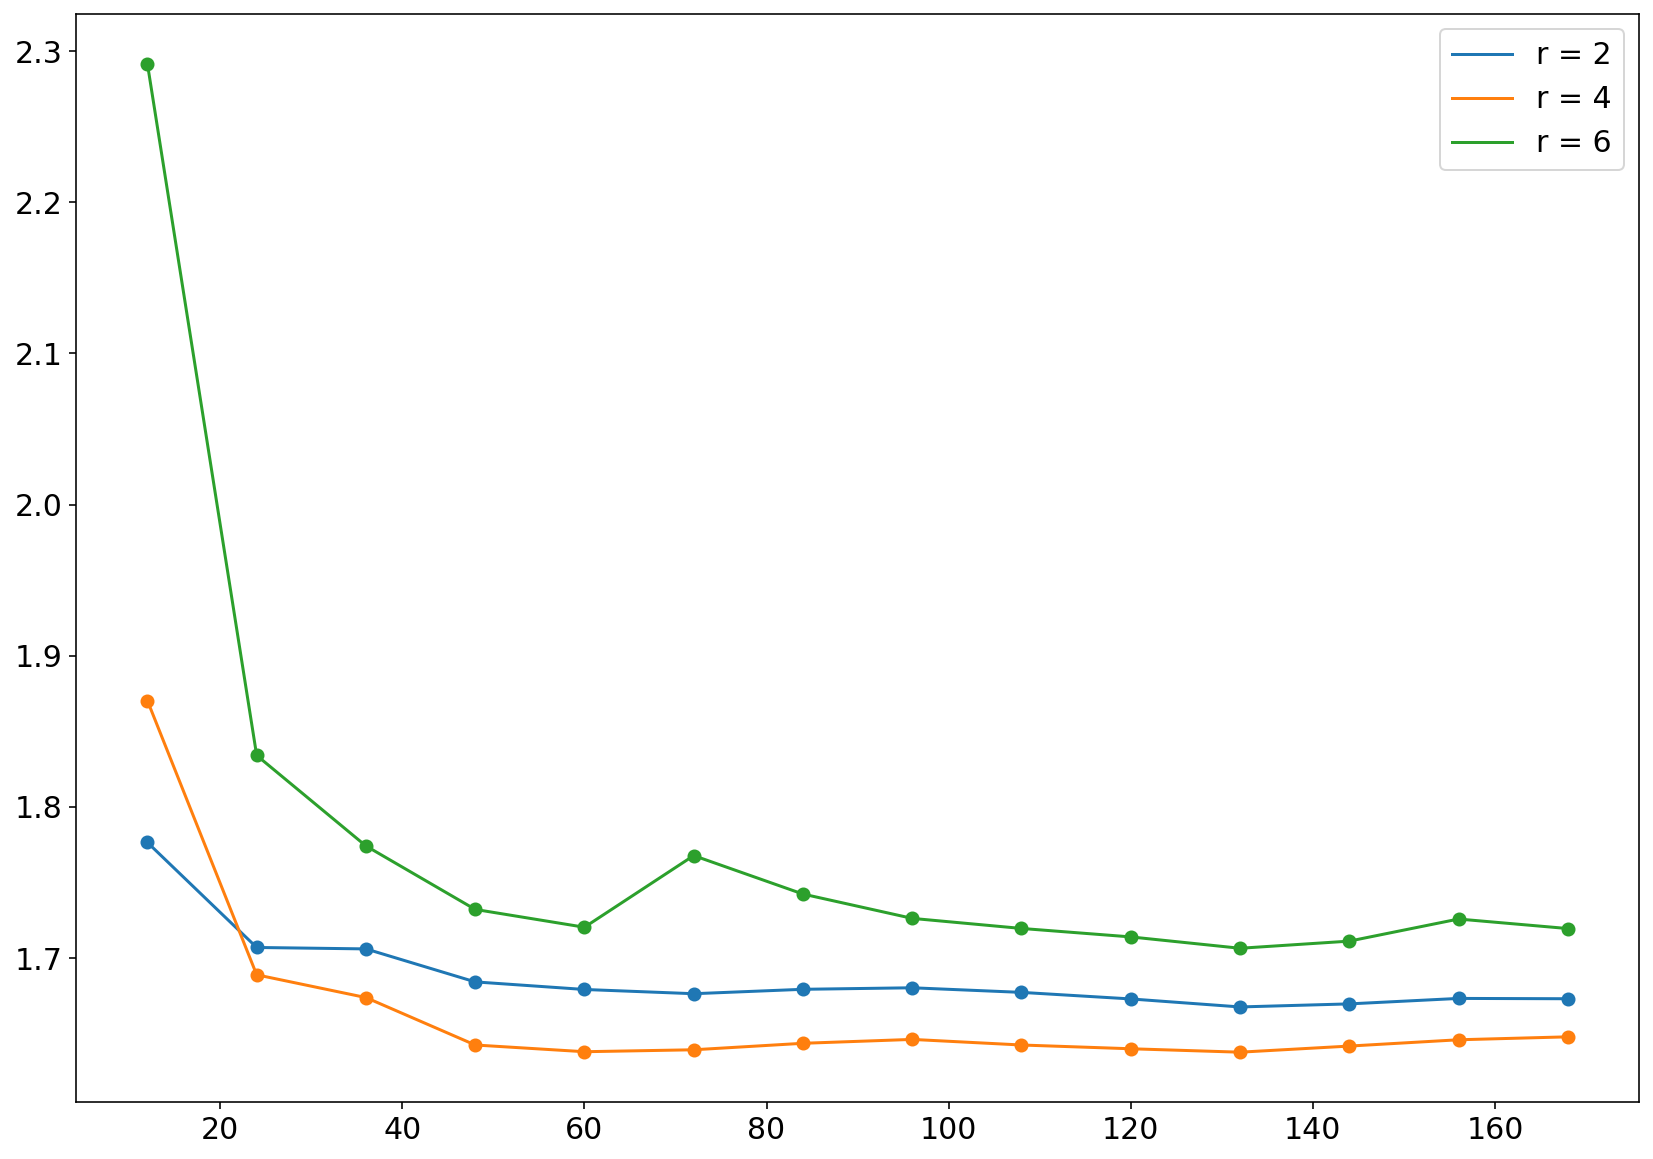
\includegraphics[width=0.9\linewidth]{imgs/comp/edsine/ssa_comp}}
	\caption{<<Сумма синусов с белым шумом>>. Ряд $\mathsf{Z}_{650}$. RMSE прогноз на валидационной части.}
	\label{edsinr_ssa_forecast}
\end{figure}

Выделим лучшее $L$ для каждого $r$. Исходя из графика, для всех $r$ можно положить $L = 132$. Также добавим $L = 175$ к лучшим параметрам и будем рассматривать комбинации параметров $L = \{132, 175\}$ и $r = \{2, 4, 6\}$.

\subsubsection{Восстановление SSA}
Посмотрим на графиках \ref{edsinr_rec2}--\ref{edsinr_rec6}, как метод SSA восстанавливает тренировочную выборку для выбранных пар параметров. На графике \ref{edsinr_rec2} видно, что при $r=2$ метод не восстанавливает ряд полностью, что естественно, так как не учтен синус с периодом 6.
%У оценки сигналы маленькая амплитуда.
На графике \ref{edsinr_rec4}, где $r = 4$, метод SSA очень хорошо аппроксимирует сигнал. А для $r = 6$ на графике \ref{edsinr_rec6} видно, что в оценку сигнала просочился шум, который мешает точность решать задачу прогнозирования. На графиках видно, что разница между параметрами $L = 132, \; L = 175$ маленькая, далее будем рассматривать только параметры $r = \{ 2, 4, 6 \}$ и $L = 175$.

\begin{figure}[H]
	\captionsetup{justification=centering}
	\center{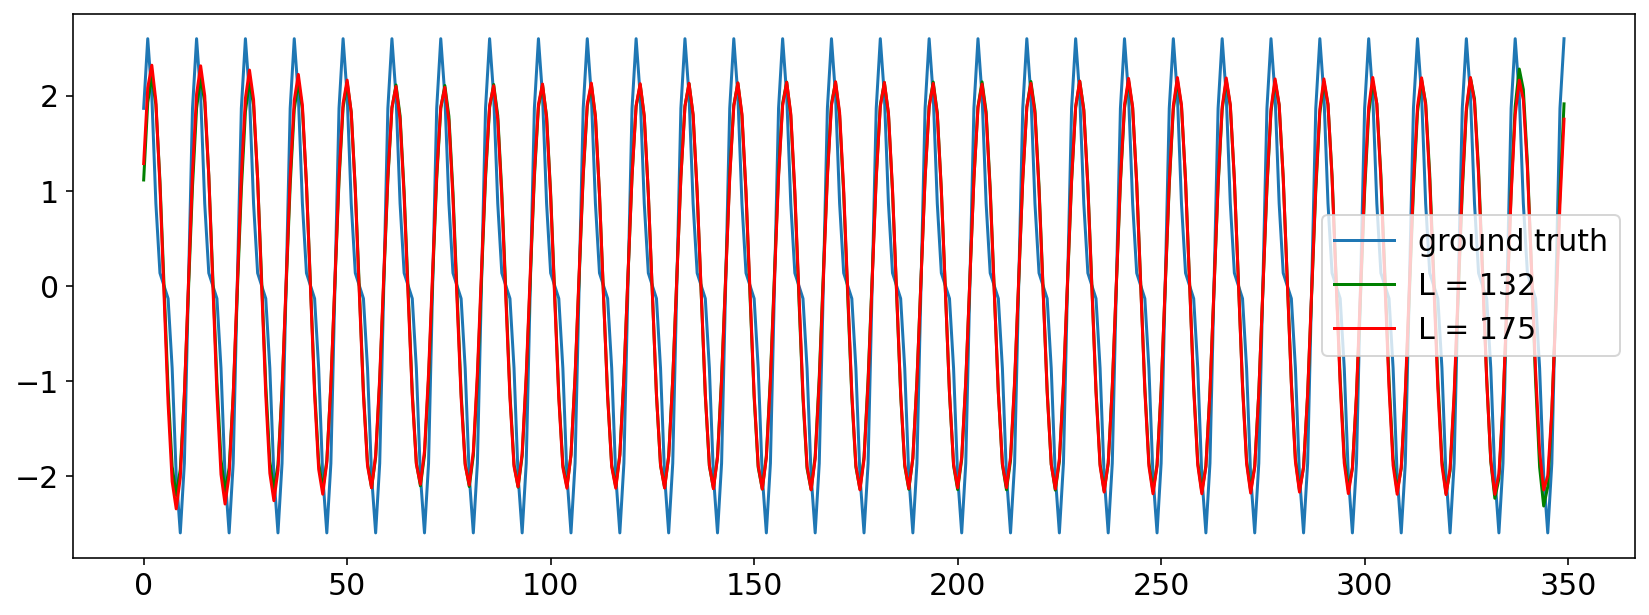
\includegraphics[width=0.9\linewidth]{imgs/comp/edsine/edsinerec2}}
	\caption{<<Сумма синусов с белым шумом>>. Ряд $\mathsf{Z}_{650}$. Восстановление тренировочной выборки с помощью метода SSA. $r = 2$}
	\label{edsinr_rec2}
\end{figure}

\begin{figure}[H]
	\captionsetup{justification=centering}
	\center{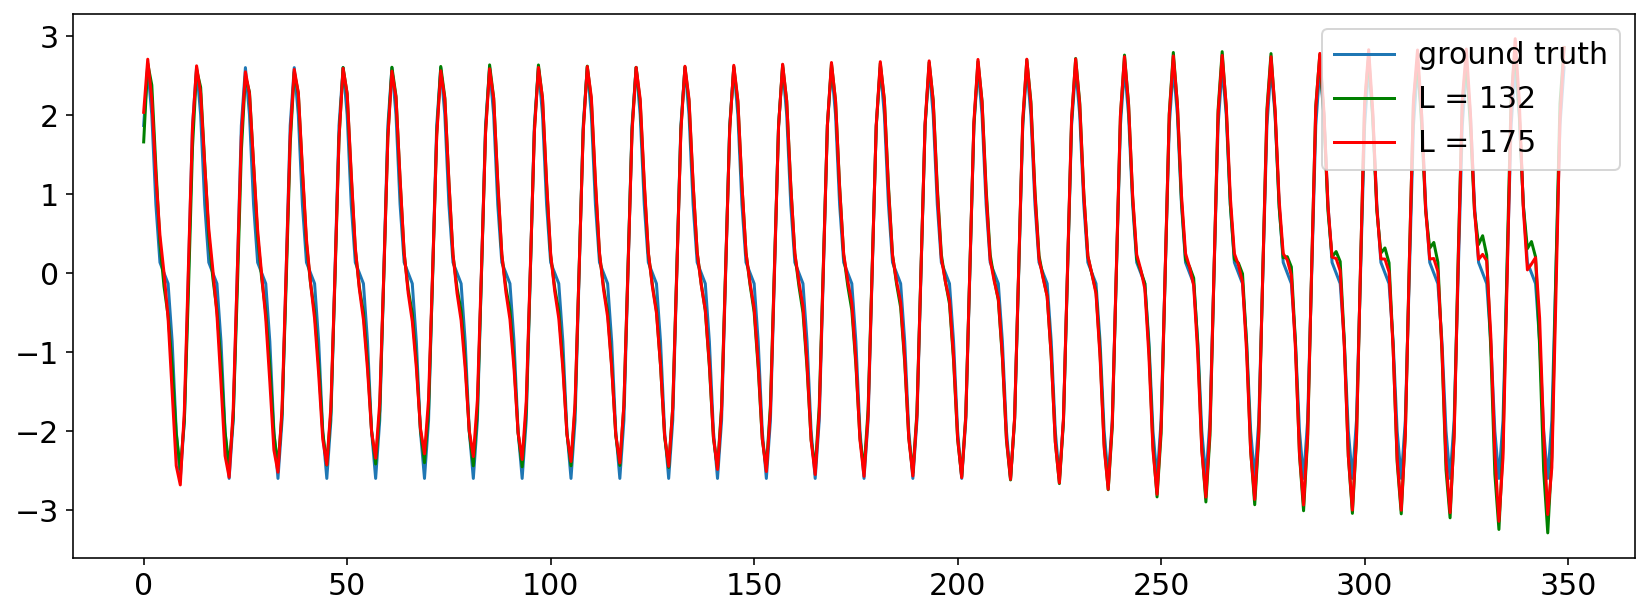
\includegraphics[width=0.9\linewidth]{imgs/comp/edsine/edsinerec4}}
	\caption{<<Сумма синусов с белым шумом>>. Ряд $\mathsf{Z}_{650}$. Восстановление тренировочной выборки с помощью метода SSA. $r = 4$}
	\label{edsinr_rec4}
\end{figure}

\begin{figure}[H]
	\captionsetup{justification=centering}
	\center{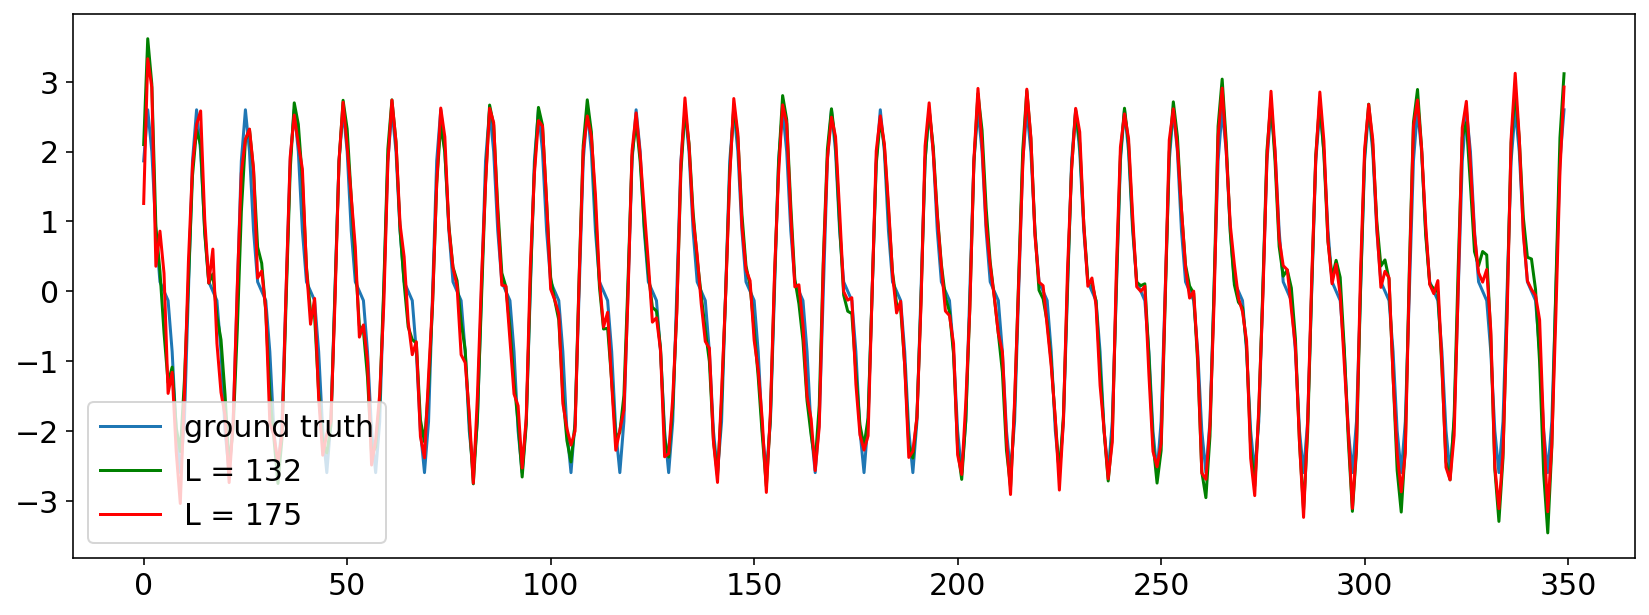
\includegraphics[width=0.9\linewidth]{imgs/comp/edsine/edsinerec6}}
	\caption{<<Сумма синусов с белым шумом>>. Ряд $\mathsf{Z}_{650}$. Восстановление тренировочной выборки с помощью метода SSA. $r = 6$}
	\label{edsinr_rec6}
\end{figure}


\subsubsection{Сравнение обычных и гибридных методов}
\label{edsiner_comp}
Для нейронных сетей зададим следующую сетку параметров: $T = \{12, 24, \ldots, 132 \}$, $h = \{10, 25, \ldots, 100 \}$. Для метода SSA в гибридных моделях возьмем пары параметров, выбранные заранее.

На графиках \multiref{edsinr_r2}{edsinr_r6} (больше графиков в приложении \ref{aedsiner_comp}), представлены результаты сравнения по сетке параметров, заданной выше. Можно заметить, что для $r = 2$ и $r = 4$ гибридные методы явно лучше, чем обычные. Для $r = 6$ результаты начинают смешиваться. В целом, для $r = 2$ и $r = 4$ ситуация выглядит похоже.
%Для $r = 4$ кривые выглядят более прямыми, что показывает меньшую зависимость ошибки от выбора параметров.

\begin{figure}[H]
	\captionsetup{justification=centering}
	\center{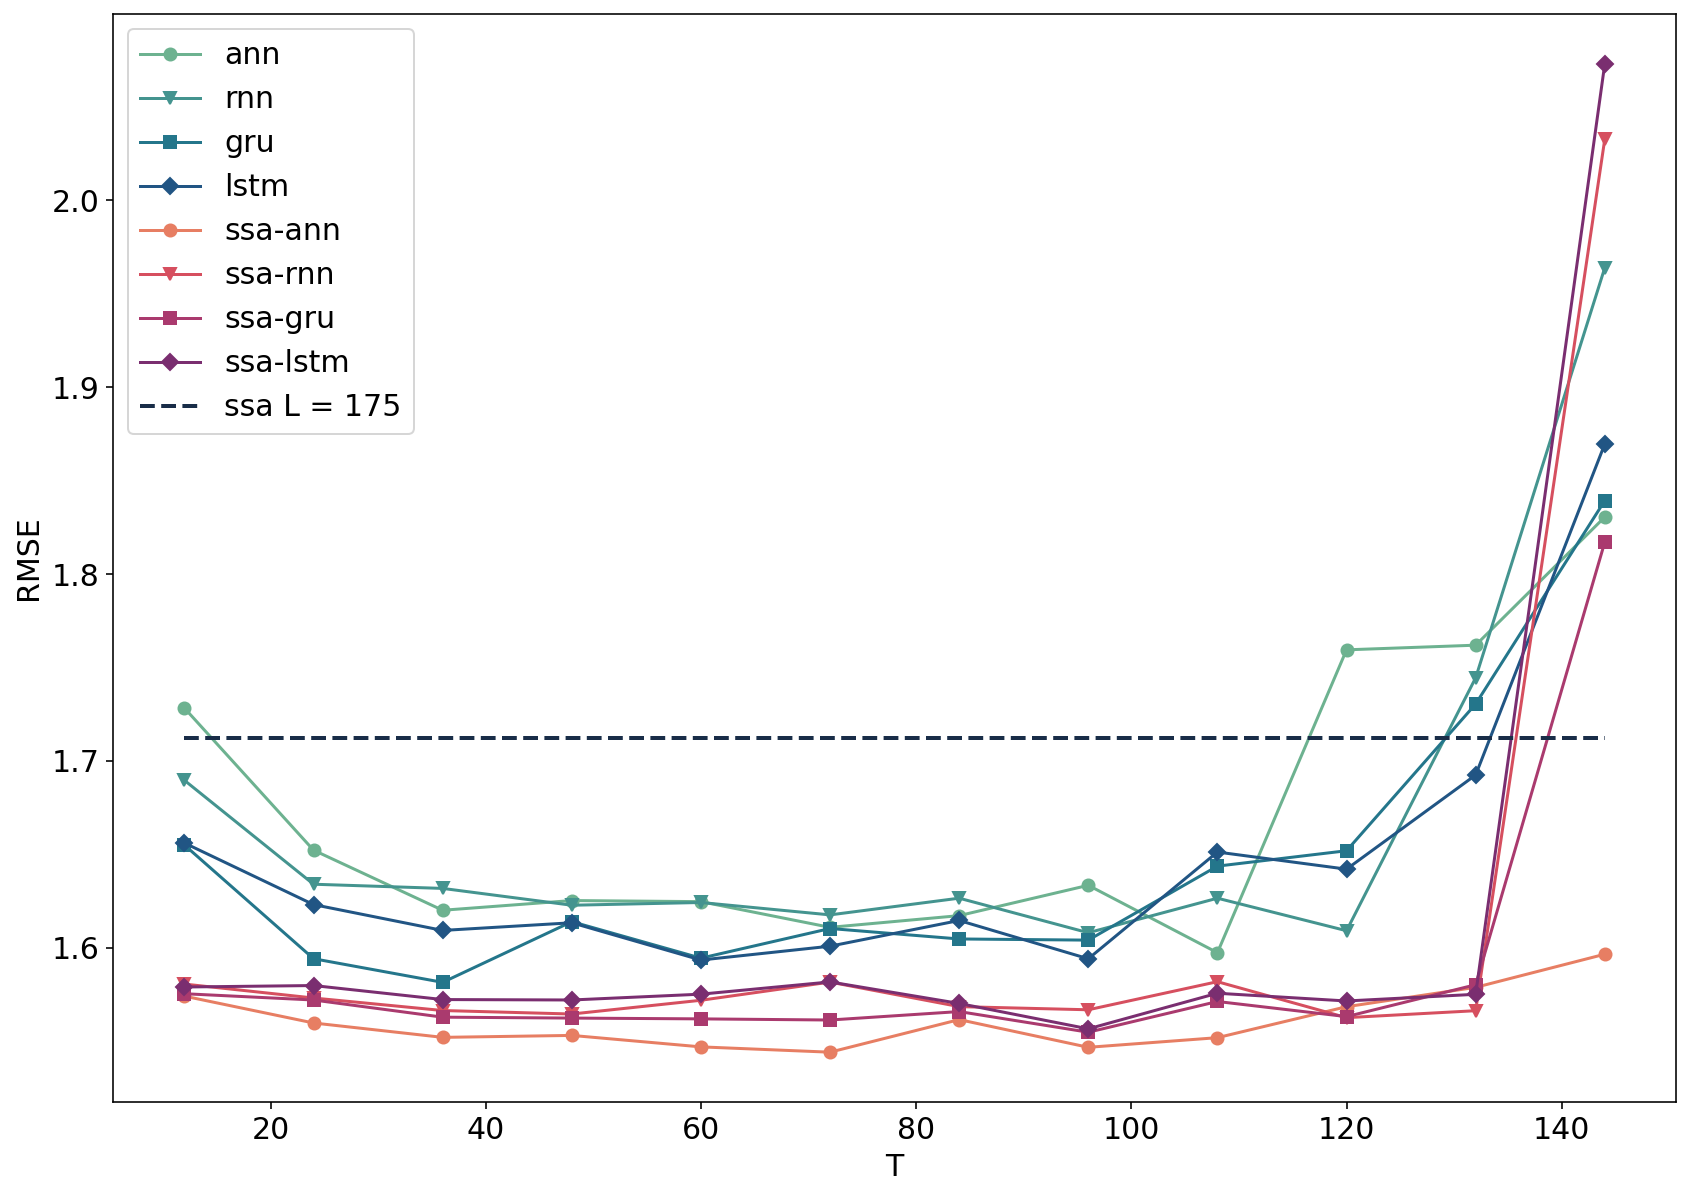
\includegraphics[width=0.9\linewidth, height=0.6\linewidth]{imgs/comp/edsine/r2}}
	\caption{<<Сумма синусов с белым шумом>>. Ряд $\mathsf{Z}_{650}$. Ошибки прогноза в зависимости от параметра $T$. $L = 175, \; r = 2$.}
	\label{edsinr_r2}
\end{figure}

\begin{figure}[H]
	\captionsetup{justification=centering}
	\center{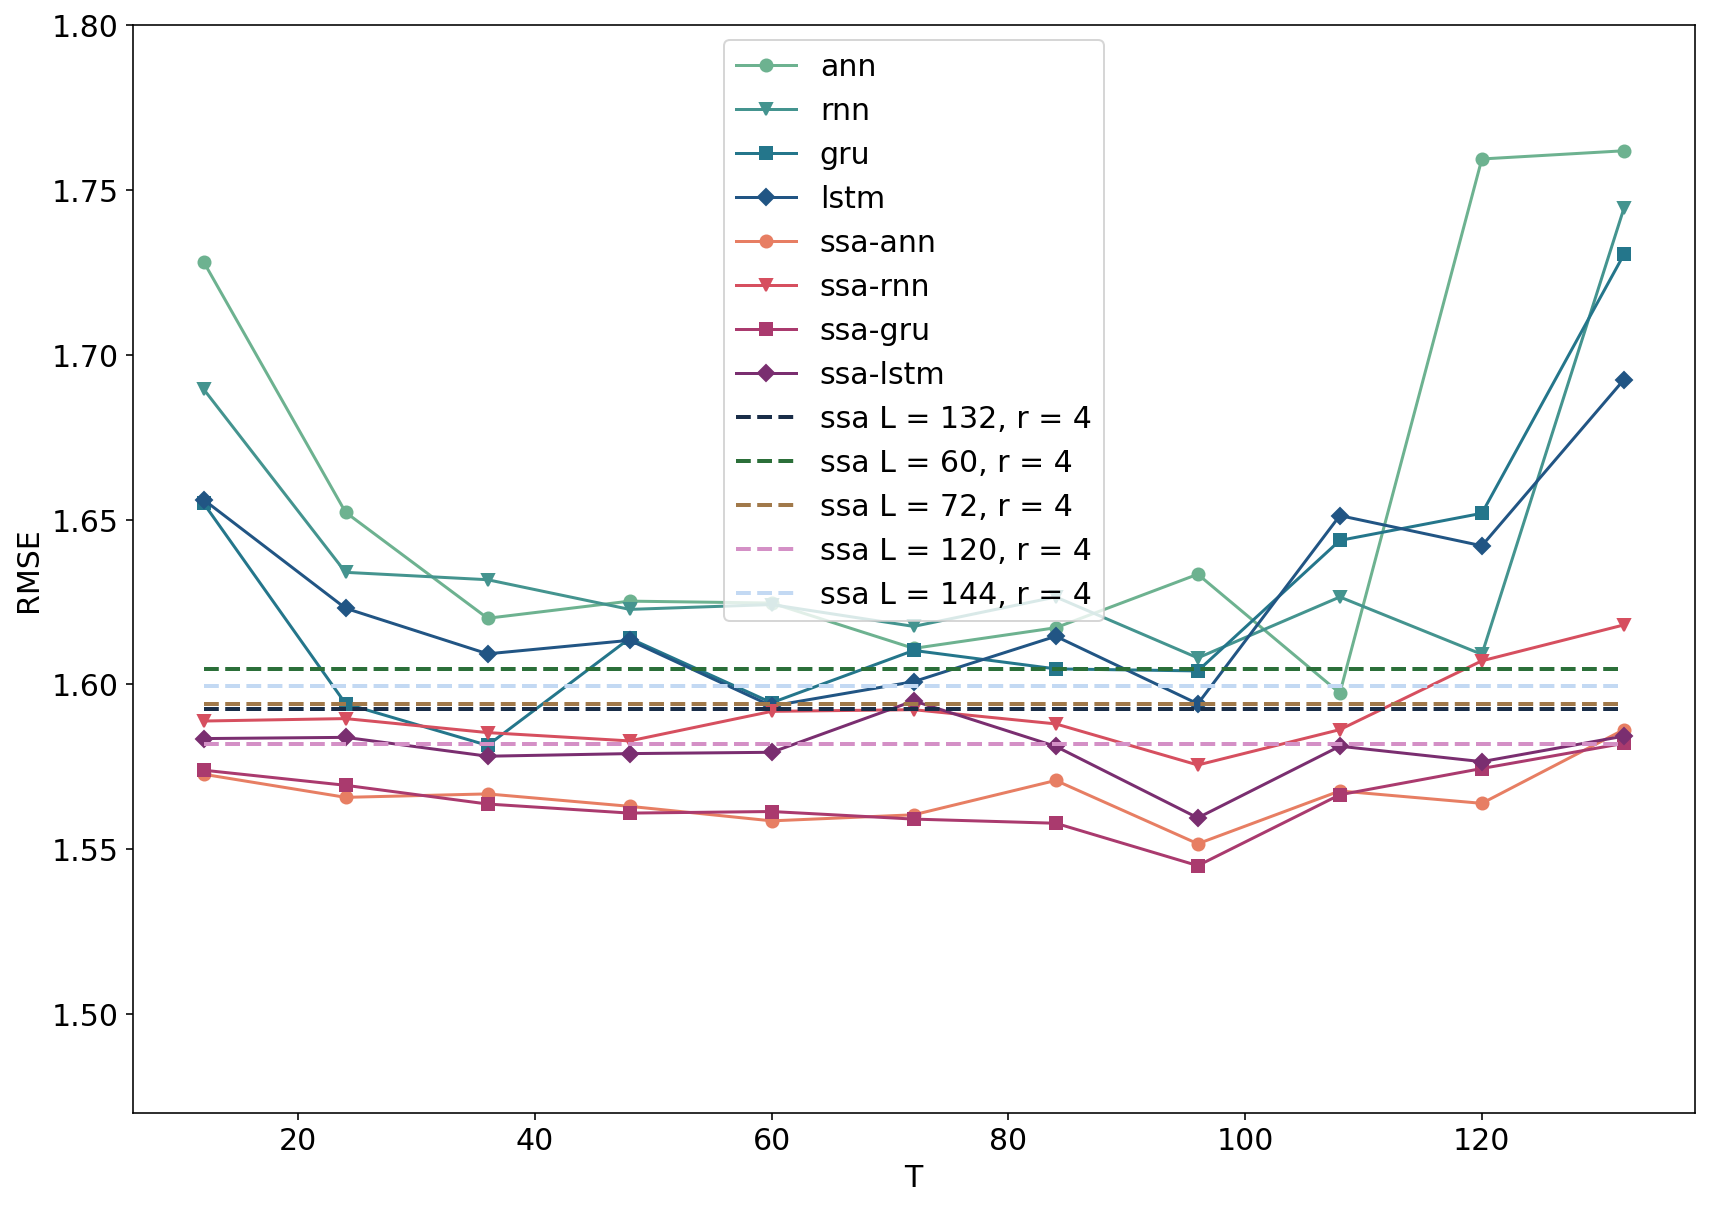
\includegraphics[width=0.9\linewidth, height=0.6\linewidth]{imgs/comp/edsine/r4}}
	\caption{<<Сумма синусов с белым шумом>>. Ряд $\mathsf{Z}_{650}$. Ошибки прогноза в зависимости от параметра $T$. $L = 175, \; r = 4$.}
	\label{edsinr_r4}
\end{figure}

\begin{figure}[H]
	\captionsetup{justification=centering}
	\center{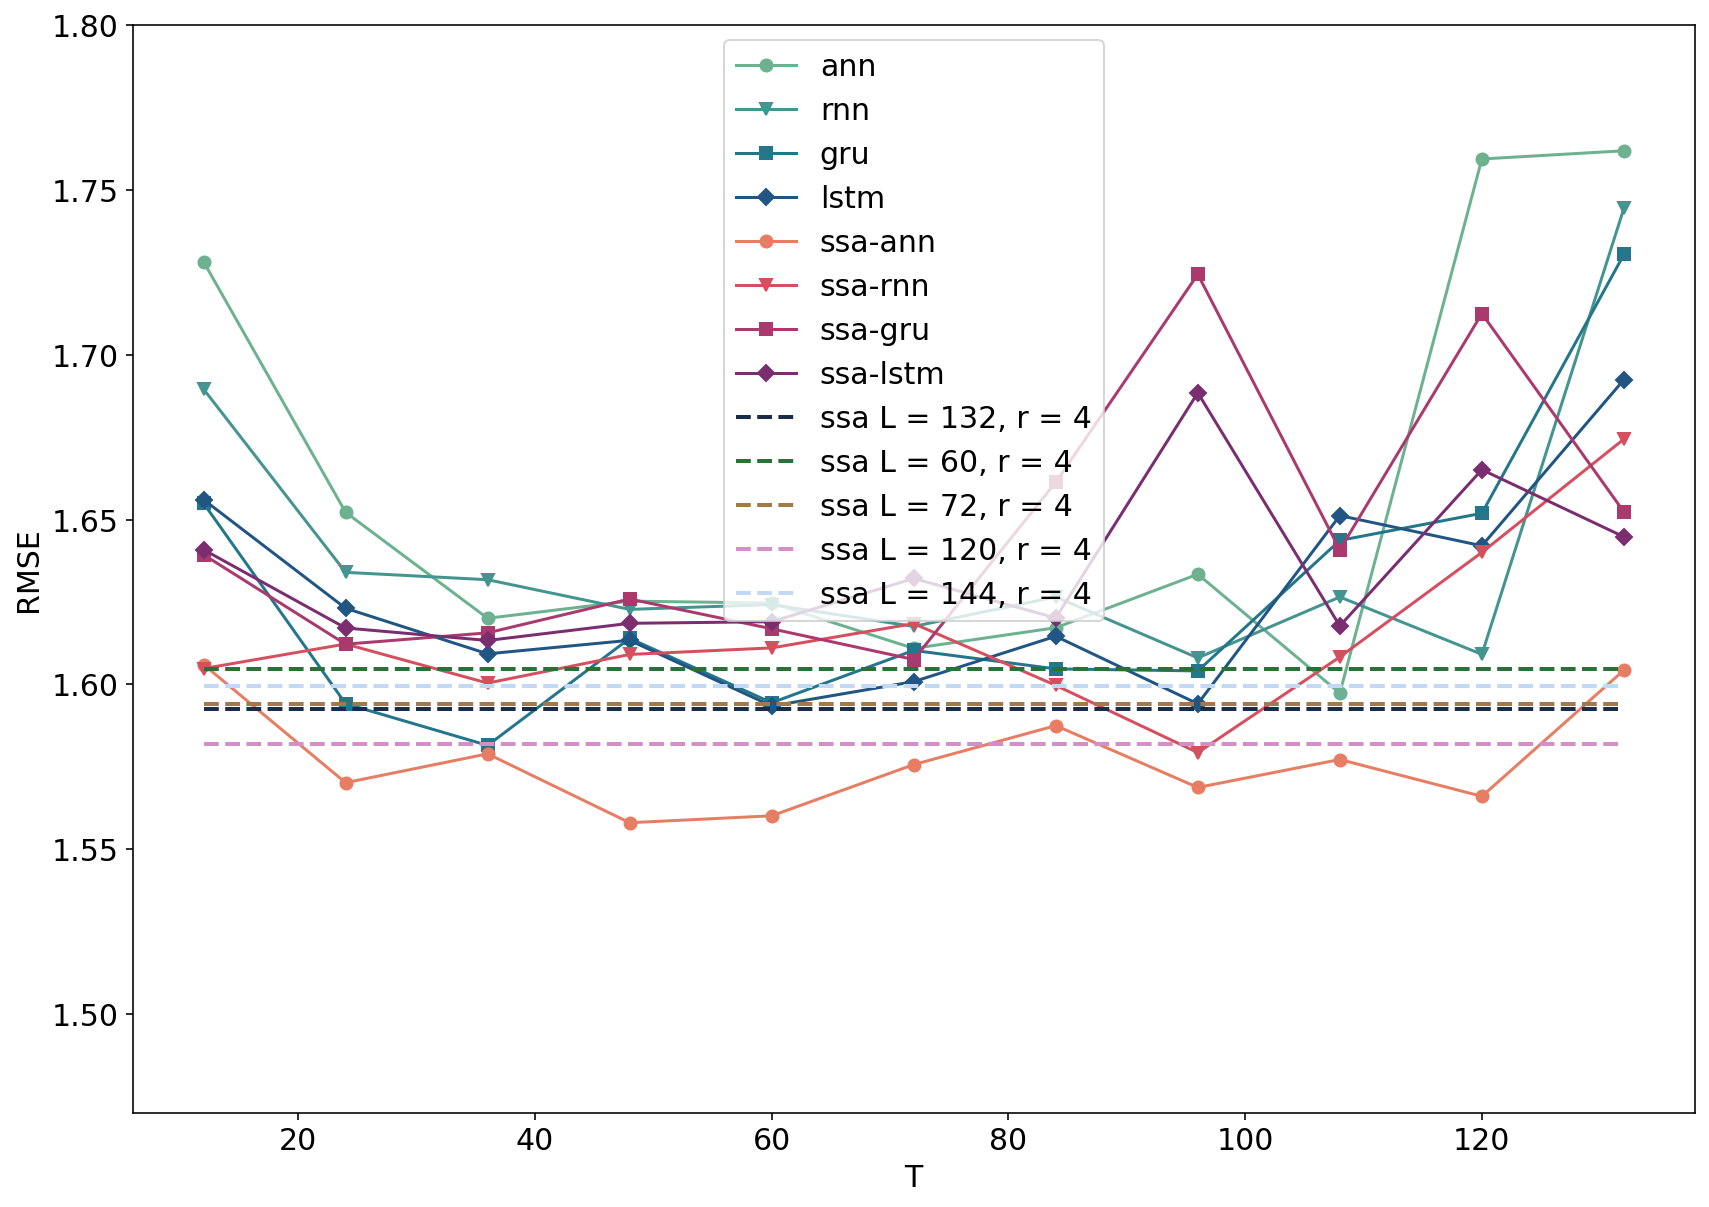
\includegraphics[width=0.9\linewidth, height=0.6\linewidth]{imgs/comp/edsine/r6}}
	\caption{<<Сумма синусов с белым шумом>>. Ряд $\mathsf{Z}_{650}$. Ошибки прогноза в зависимости от параметра $T$. $L = 175, \; r = 6$.}
	\label{edsinr_r6}
\end{figure}

\subsubsection{Отображение прогнозов}
\label{edsiner_res}

На графиках \multiref{edsinr_r2_res_ann}{edsinr_r6_res_ann} (больше графиков в приложении \ref{aedsiner_res}) представлены результаты прогнозирования методам ANN. На графиках можно подтвердить выводы полученные ранее. Так на графиках для $r = 6$ видно, что в прогноз просочился шум. Прогнозы для $r = 2$ и $r = 4$ выглядят похоже, но в случае $r = 2$ форма прогноза больше похожа на форму сигнала.
%на метод повторяет <<ступеньку>>.
Прогноз для $r = 4$ выглядит более гладким.

\begin{figure}[H]
	\captionsetup{justification=centering}
	\center{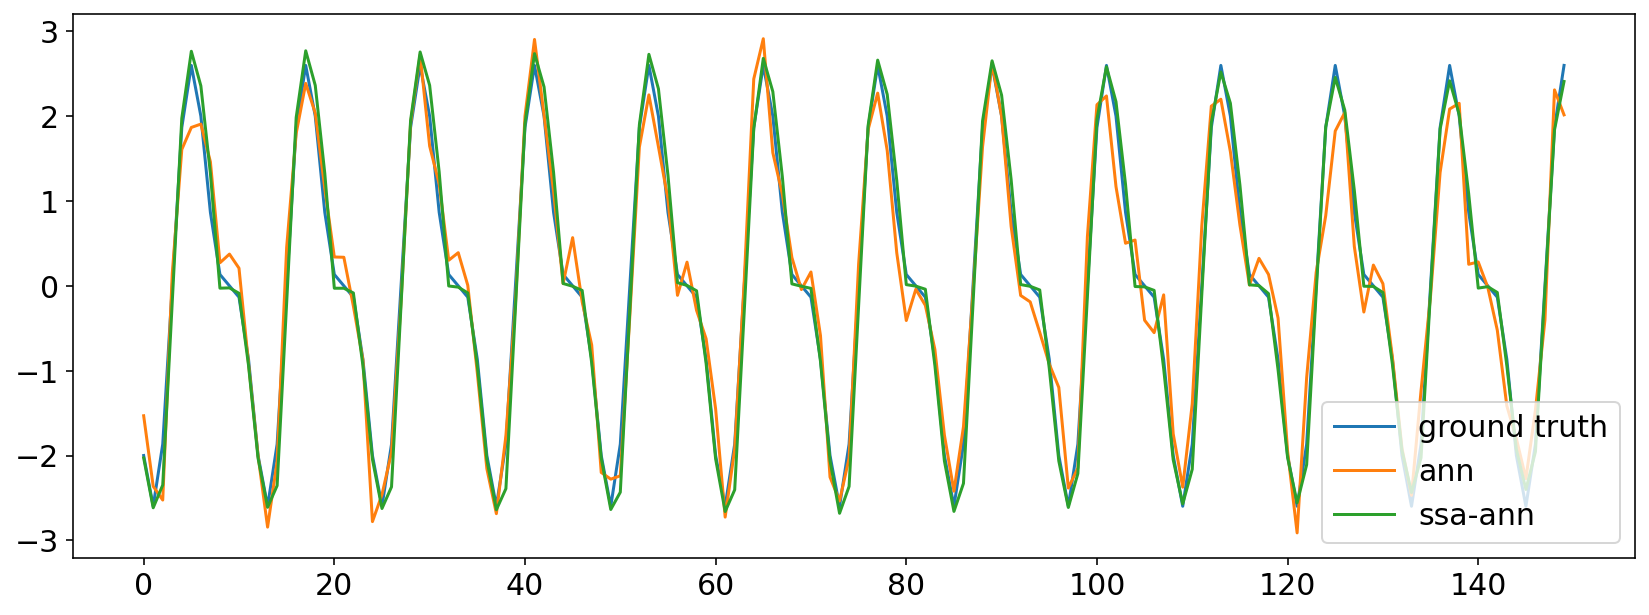
\includegraphics[width=0.9\linewidth]{imgs/comp/edsine/edsinr_r2_res_ann}}
	\caption{<<Сумма синусов с белым шумом>>. Ряд $\mathsf{Z}_{650}$. Прогноз для ANN и SSA-ANN. $r = 2$}
	\label{edsinr_r2_res_ann}
\end{figure}

\begin{figure}[H]
	\captionsetup{justification=centering}
	\center{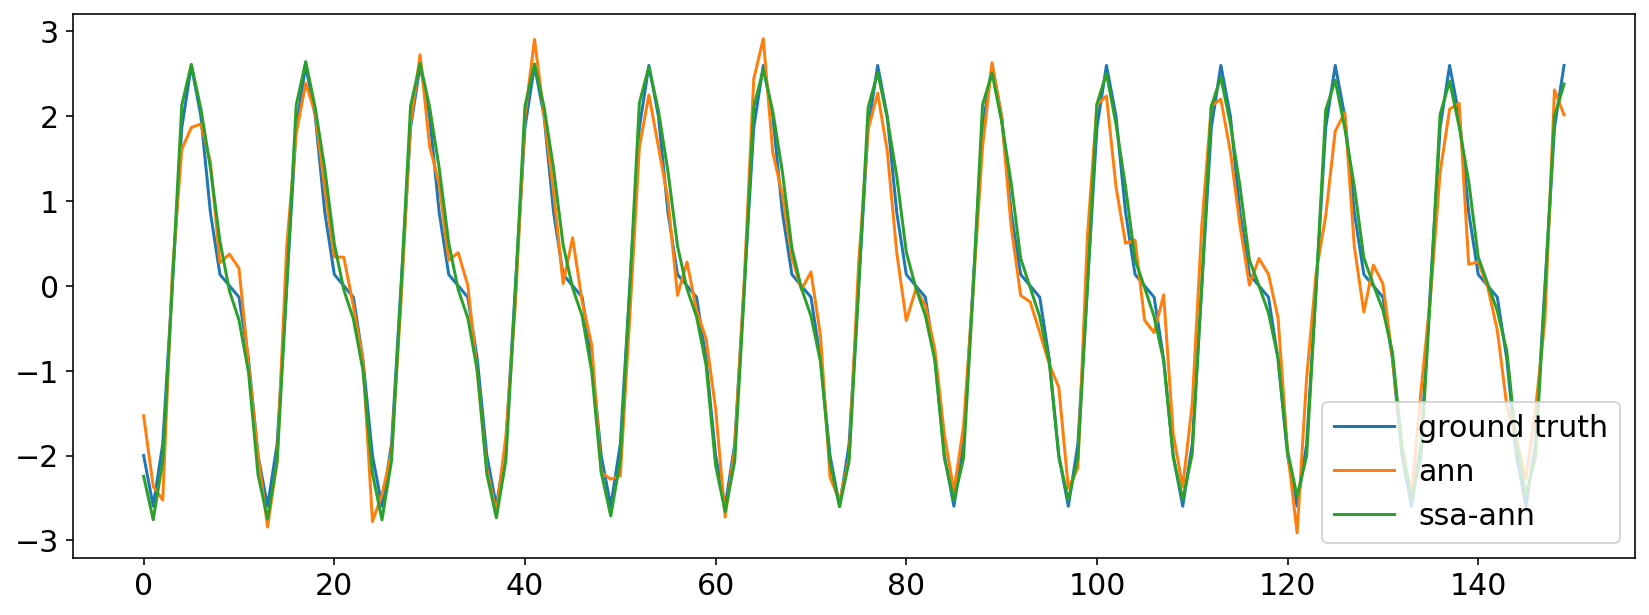
\includegraphics[width=0.9\linewidth]{imgs/comp/edsine/edsinr_r4_res_ann}}
	\caption{<<Сумма синусов с белым шумом>>. Ряд $\mathsf{Z}_{650}$. Прогноз для ANN и SSA-ANN. $r = 4$}
	\label{edsinr_r4_res_ann}
\end{figure}

\begin{figure}[H]
	\captionsetup{justification=centering}
	\center{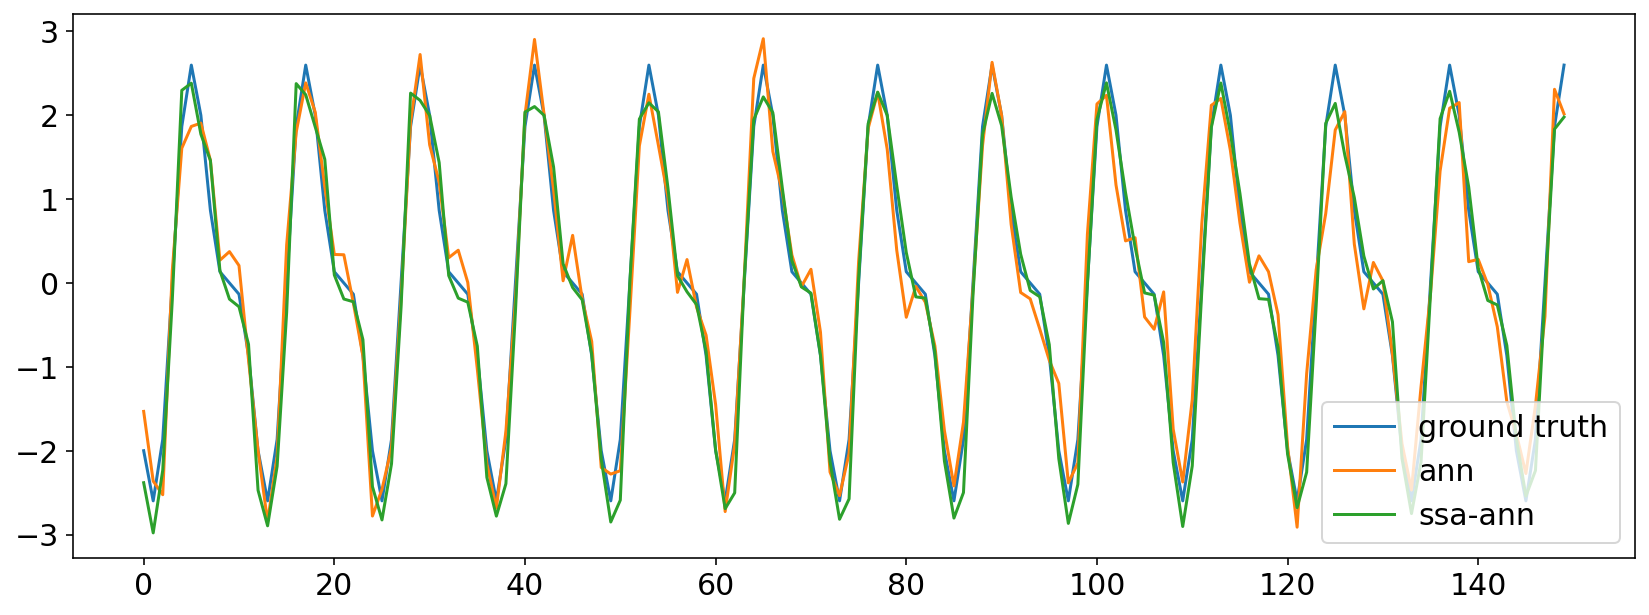
\includegraphics[width=0.9\linewidth]{imgs/comp/edsine/edsinr_r6_res_ann}}
	\caption{<<Сумма синусов с белым шумом>>. Ряд $\mathsf{Z}_{650}$. Прогноз для ANN и SSA-ANN. $r = 6$}
	\label{edsinr_r6_res_ann}
\end{figure}

\subsubsection{Проверка устойчивости}
\label{edsiner_rob}

Чтобы исключить случайность в полученных результатах, проведем сравнение для разных начальных весов методов. Зафиксируем уменьшенную сетку для параметра $T = \{12, 84\}$. Сетка для параметра $h$ останется прежней. Будем получать каждый результат по 7 раз, инициализируя метод с новыми весами. Полученные результаты отображены на рисунках \multiref{edsiner4.12}{edsiner4.84} (больше графиков в приложении \ref{aedsiner_rob}). На них подтверждается выводы, сделанные ранее. Заключаем, что полученные результаты устойчивые.

\begin{figure}[h]
	\captionsetup{justification=centering}
	\center{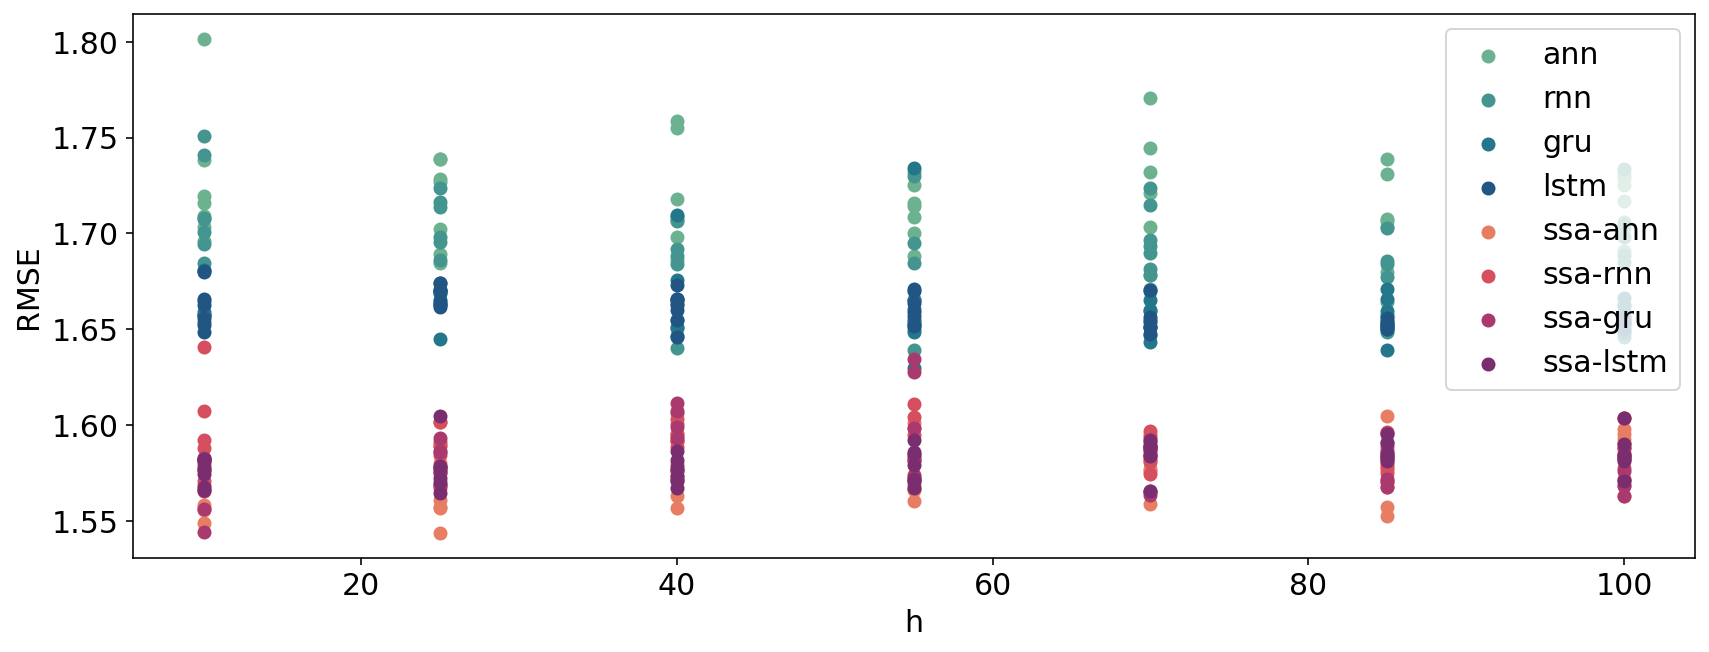
\includegraphics[width=0.9\linewidth]{imgs/comp/edsine/loopr4.12}}
	\caption{<<Сумма синусов с белым шумом>>. Ряд $\mathsf{Z}_{650}$. Проверка устойчивости. $r = 4, \; L = 175$. $T = 12$.}
	\label{edsiner4.12}
\end{figure}

\begin{figure}[h]
	\captionsetup{justification=centering}
	\center{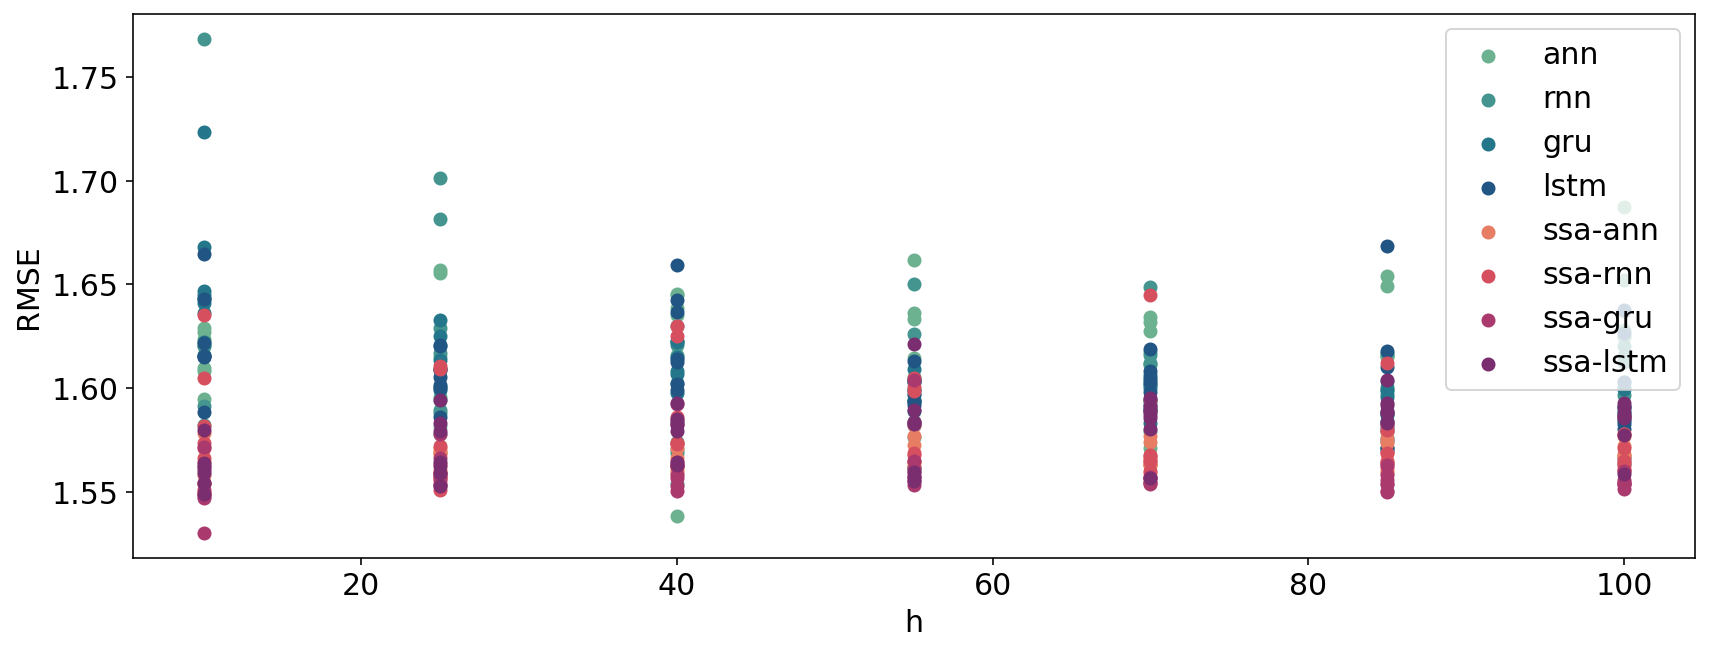
\includegraphics[width=0.9\linewidth]{imgs/comp/edsine/loopr4.84}}
	\caption{<<Сумма синусов с белым шумом>>. Ряд $\mathsf{Z}_{650}$. Проверка устойчивости. $r = 4, \; L = 175$. $T = 84$.}
	\label{edsiner4.84}
\end{figure}

\subsubsection{Выводы}
На ряде $\mathsf{Z}_{650}$ было продемонстрировано сравнение обычных и гибридных методов, и метода SSA. В таблице \ref{tedsiner} продемонстрированы величины ошибок по метрике RMSE для методов.

Из значений в таблицы~\ref{tedsiner} и полученных ранее результатов можем сделать выводы, что для ряда с несложно выделяемым сигналом выбор аналитически верных параметров приводит к одному из лучших результатов. Что удивительно, выбор ранга $r=2$ меньше ранга сигнала привел к улучшению, хоть и небольшому, точности прогноза. При этом остаётся непонятным, каким образом нейронные сети делают прогноз с хорошей точностью при том, что на вход подаётся неправильное восстановление сигнала в результате предобработки SSA.

Гибридные методы показали наилучшую точность. Наибольшую ошибку показал метод SSA. Как и говорилось, наименьшая ошибка достигается для $r = 2$ в гибридных моделях. Средняя ошибка для $r = 2$ и $r = 4$ не сильно отличается. Для $r = 6$ средняя ошибка гибридных методов выше.

Таблица~\ref{bigtable} показывает, что из негибридных методов хорошо работают GRU и LSTM, однако в паре с SSA лучший результат у ANN.

\begin{table}[H]
	\captionsetup{justification=centering}
	\caption{<<Сумма синусов с белым шумом>>. Ряд $\mathsf{Z}_{650}$. Усредненные и лучшие результаты прогнозов по RMSE.}
	\begin{center}
		\begin{tabular}{ccccc}
			\toprule
			{ssa-params} &  b-nn &  m-nn &  b-ssa &  m-ssa \\
			\midrule
			-          & 1.547 & 1.635 &  1.581 &  1.586 \\
			$ L = 175, \; r = 2$         & 1.528 & 1.567 &  1.581 &  1.586 \\
			$ L = 175, \; r = 4$        & 1.532 & 1.575 &  1.581 &  1.586 \\
			$ L = 175, \; r = 6$        & 1.533 & 1.613 &  1.581 &  1.586 \\
			\bottomrule
		\end{tabular}
	\end{center}
	\label{tedsiner}
\end{table}


\subsection{Влияние выбора параметра $r$ для ряда с небольшим шумом}
\label{edsinr_lownoise}
Поставим задачу сравнить обычные и гибридные методы в случае разных выбранных параметрах $r$ в гибридных методах на временном ряде с небольшим шумом. Эксперимент аналогичен описанному в разделе \ref{edsinr}. Будем проводить сравнение на ряде $\mathsf{X}_{650}$.

\subsubsection{Прогноз по SSA}

Сравним точность прогнозирования методом SSA при разных параметрах $r$. Зададим следующую сетку параметров $L = \{12, 24, \ldots, 175\}$, $r = \{2, 4, 6\}$. Посмотрим на результаты на рисунке \ref{edsin0.3r_ssa_forecast}. На графике видно, что наилучшие результаты достигаются при $r = 4$, худшие результаты достигаются при $r = 2$, что отличает этот пример от предыдущего с б\'{о}льшим шумом.


\begin{figure}[H]
	\captionsetup{justification=centering}
	\center{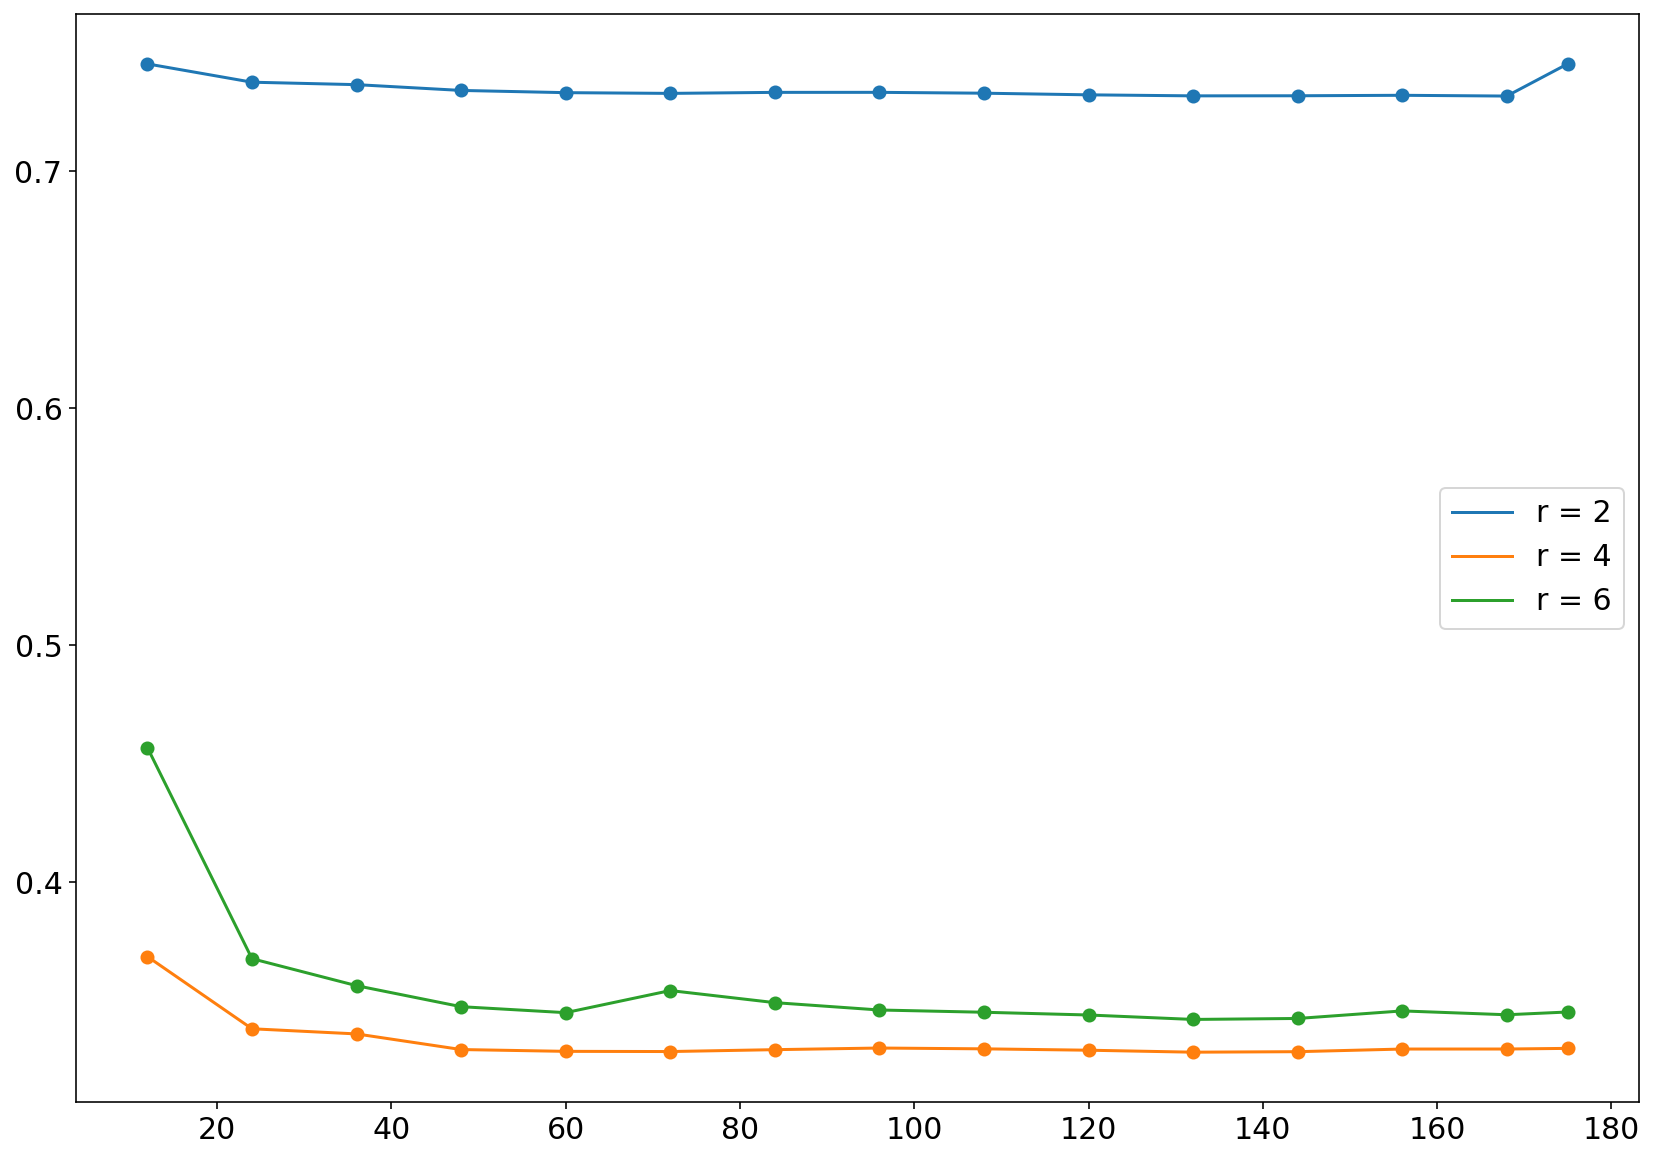
\includegraphics[width=0.9\linewidth]{imgs/comp/edsine/N0.3/ssa_comp}}
	\caption{<<Сумма синусов с небольшим белым шумом>>. Ряд $\mathsf{X}_{650}$. RMSE прогноз на валидационной части.}
	\label{edsin0.3r_ssa_forecast}
\end{figure}

Выделим лучшее $L$ для каждого $r$. Исходя из графика для $r = \{4, 6\}$ это будет $L = 132$, для $r = 2$ будет $L = 168$. Также добавим $L = 175$ к лучшим параметрам и будем рассматривать комбинации параметров $L = \{132, 168, 175\}$ и $r = \{2, 4, 6\}$.

\subsubsection{Восстановление SSA}
Посмотрим, как метод SSA восстанавливает тренировочную выборку для выбранных пар на графиках ниже. На графике \ref{edsin0.3r_rec2} видно, что метод не восстанавливает ряд полностью. Результат очень похожи на те, что в разделе \ref{edsinr}. На графиках \ref{edsin0.3r_rec4}, \ref{edsin0.3r_rec6}, видно, что восстановление очень хорошее. На графике \ref{edsin0.3r_rec6} можно заметить влияние шума, видно, как в оценках сигнала дрожат пики. На графиках видно, что разницы между параметрами $L$ нет, далее будем рассматривать только параметры $r = \{ 2, 4, 6 \}$ и $L = 175$.

\begin{figure}[H]
	\captionsetup{justification=centering}
	\center{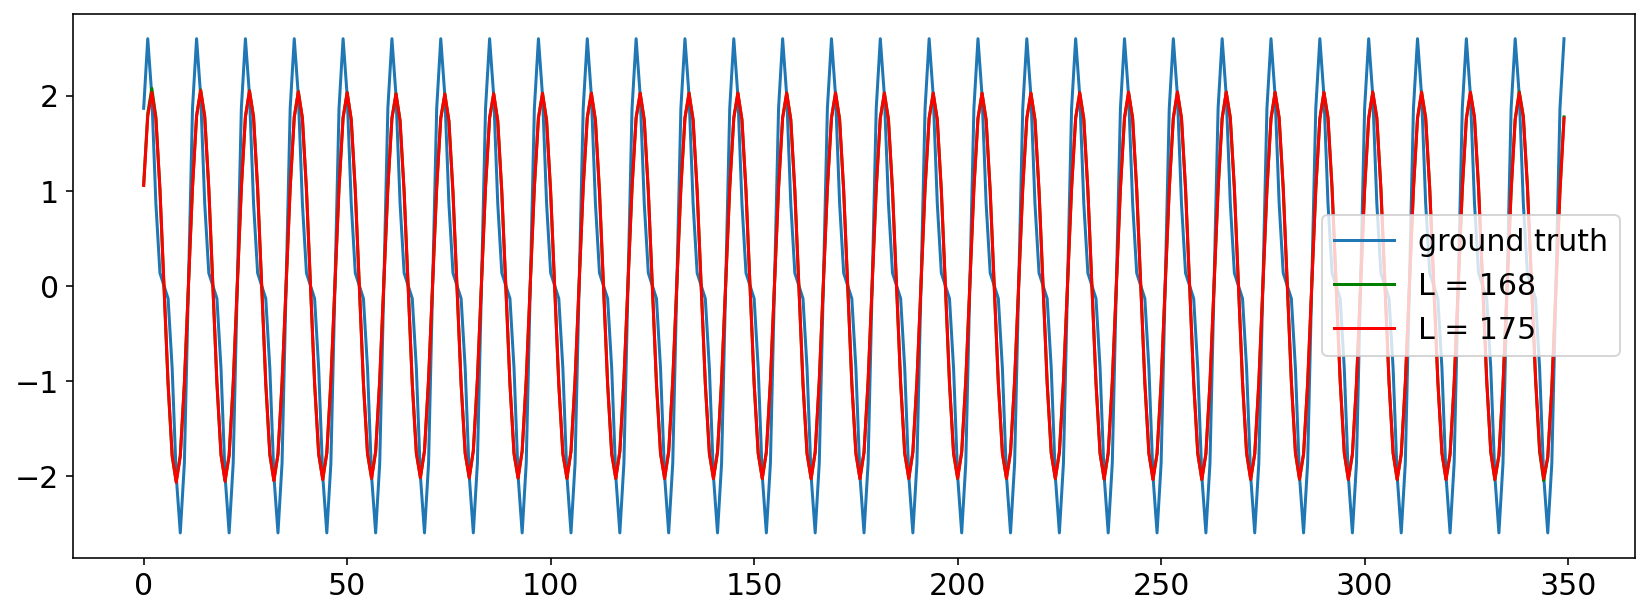
\includegraphics[width=0.9\linewidth]{imgs/comp/edsine/N0.3/edsinerec2}}
	\caption{<<Сумма синусов с небольшим белым шумом>>. Ряд $\mathsf{X}_{650}$. Восстановление тренировочной выборки с помощью метода SSA. $r = 2$}
	\label{edsin0.3r_rec2}
\end{figure}

\begin{figure}[H]
	\captionsetup{justification=centering}
	\center{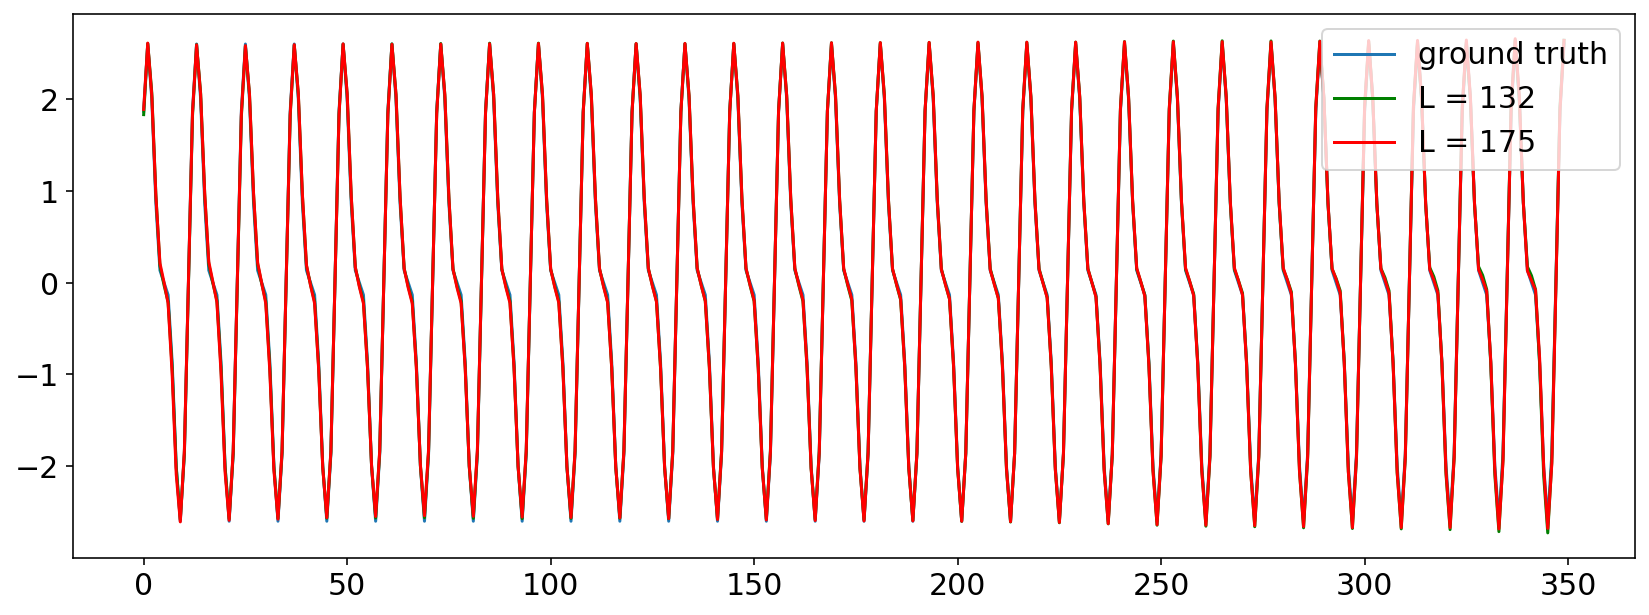
\includegraphics[width=0.9\linewidth]{imgs/comp/edsine/N0.3/edsinerec4}}
	\caption{<<Сумма синусов с небольшим белым шумом>>. Ряд $\mathsf{X}_{650}$. Восстановление тренировочной выборки с помощью метода SSA. $r = 4$}
	\label{edsin0.3r_rec4}
\end{figure}

\begin{figure}[H]
	\captionsetup{justification=centering}
	\center{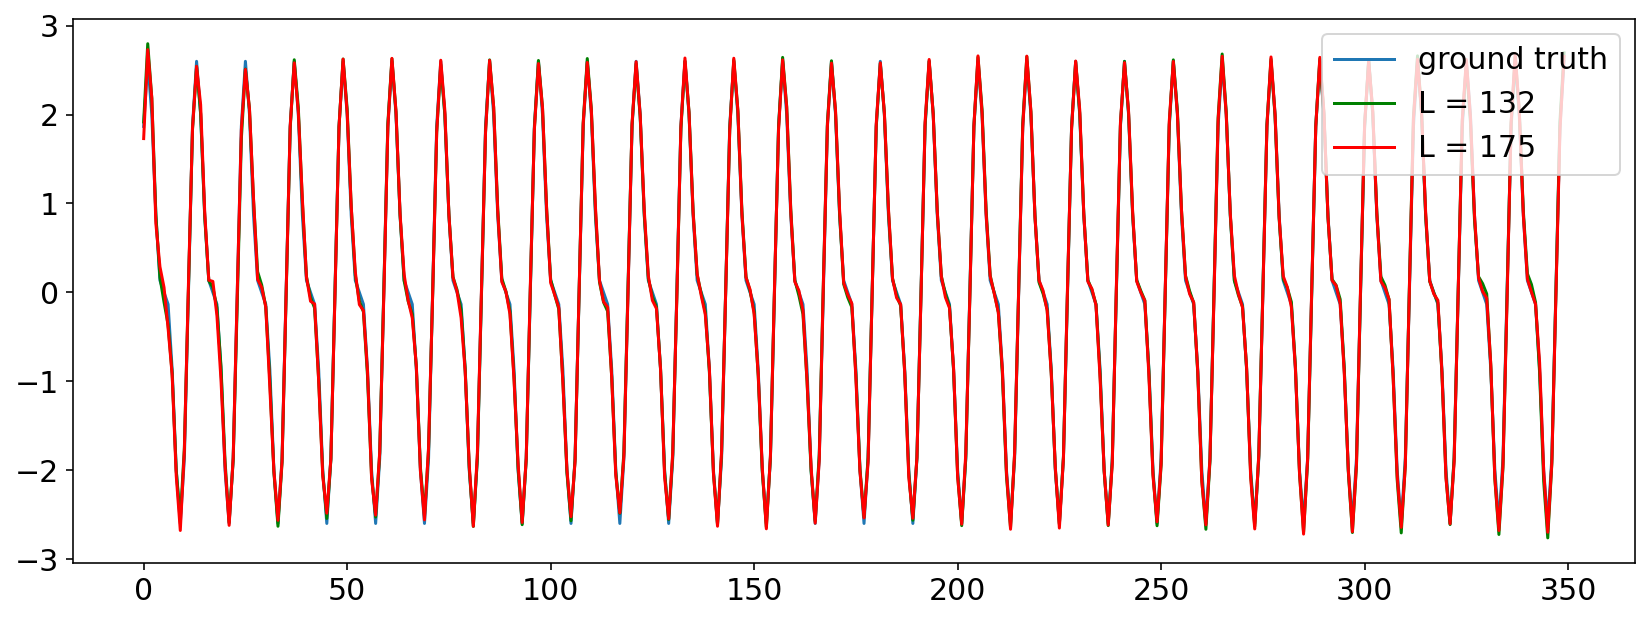
\includegraphics[width=0.9\linewidth]{imgs/comp/edsine/N0.3/edsinerec6}}
	\caption{<<Сумма синусов с небольшим белым шумом>>. Ряд $\mathsf{X}_{650}$. Восстановление тренировочной выборки с помощью метода SSA. $r = 6$}
	\label{edsin0.3r_rec6}
\end{figure}

\subsubsection{Сравнение обычных и гибридных методов}
\label{edsine0.3r_comp}

Для нейронных сетей зададим следующую сетку параметров: $T = \{12, 24, \ldots, 132 \}$, $h = \{10, 25, \ldots, 100 \}$. Для метода SSA в гибридных моделях возьмем пары параметров, выбранные заранее.

На графиках \multiref{edsin0.3r_r2}{edsin0.3r_r6} (больше графиков в приложении \ref{aedsine0.3r_comp}) представлены результаты сравнения по сетке параметров, заданной выше. Можно заметить, что гибридные методы явно лучше, чем обычные. В целом, результаты аналогичны результатам в разделе \ref{edsinr}.

\begin{figure}[H]
	\captionsetup{justification=centering}
	\center{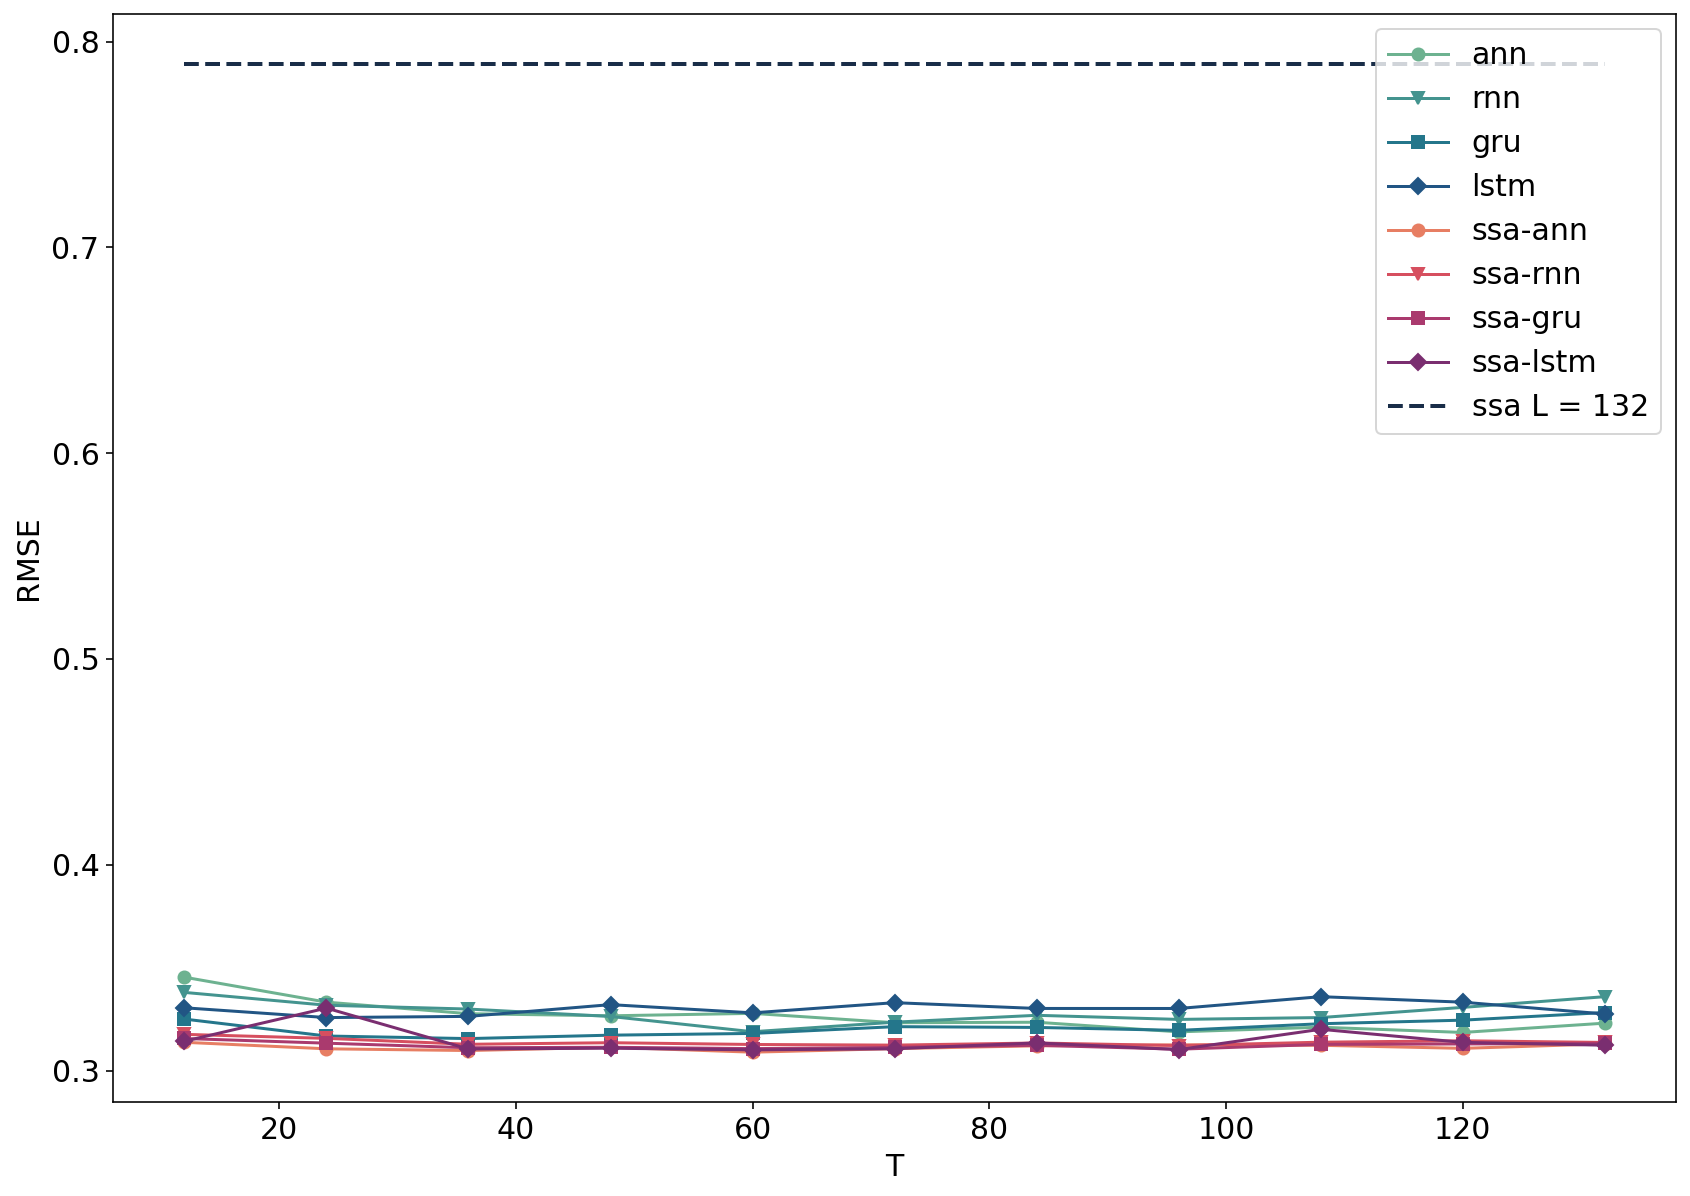
\includegraphics[width=0.9\linewidth, height=0.6\linewidth]{imgs/comp/edsine/N0.3/r2}}
	\caption{<<Сумма синусов с небольшим белым шумом>>. Ряд $\mathsf{X}_{650}$. Ошибки прогноза в зависимости от параметра $T$. $L = 175, \; r = 2$.}
	\label{edsin0.3r_r2}
\end{figure}

\begin{figure}[H]
	\captionsetup{justification=centering}
	\center{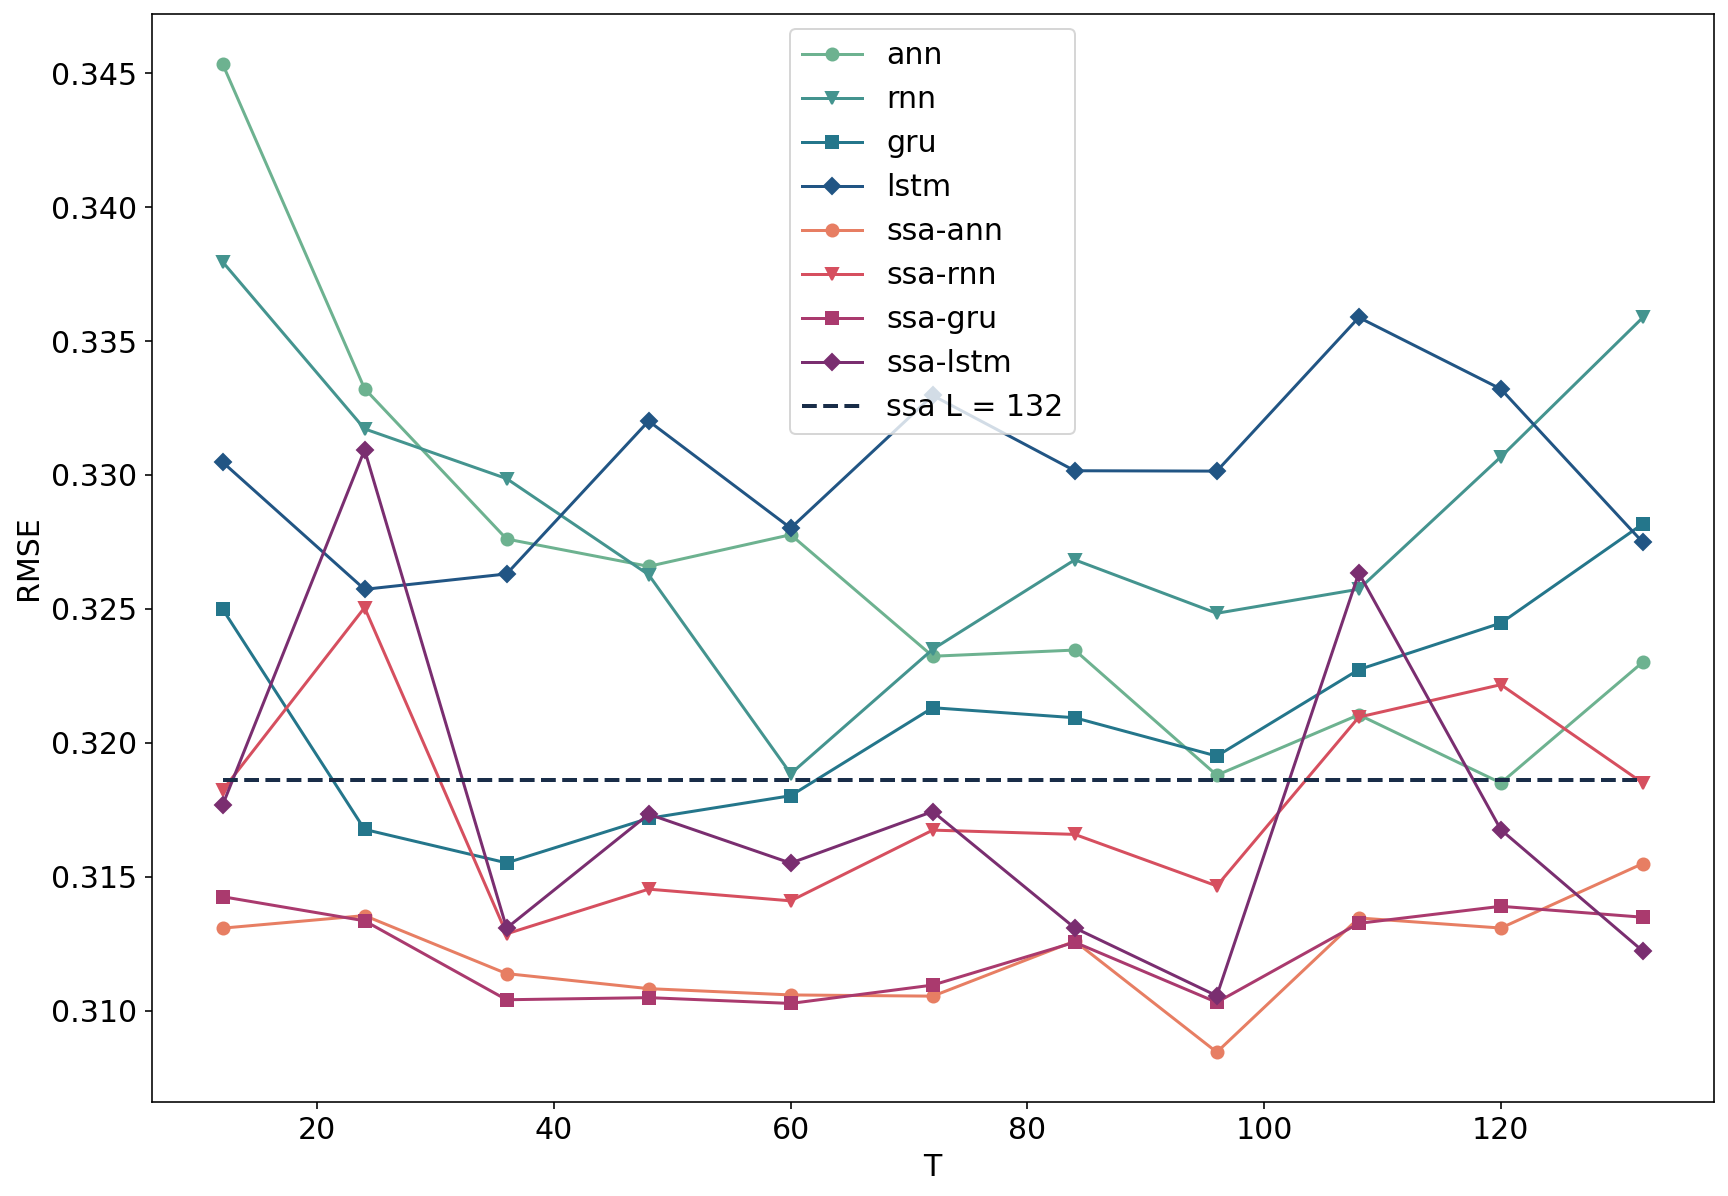
\includegraphics[width=0.9\linewidth, height=0.6\linewidth]{imgs/comp/edsine/N0.3/r4}}
	\caption{<<Сумма синусов с небольшим белым шумом>>. Ряд $\mathsf{X}_{650}$. Ошибки прогноза в зависимости от параметра $T$. $L = 175, \; r = 4$.}
	\label{edsin0.3r_r4}
\end{figure}

\begin{figure}[H]
	\captionsetup{justification=centering}
	\center{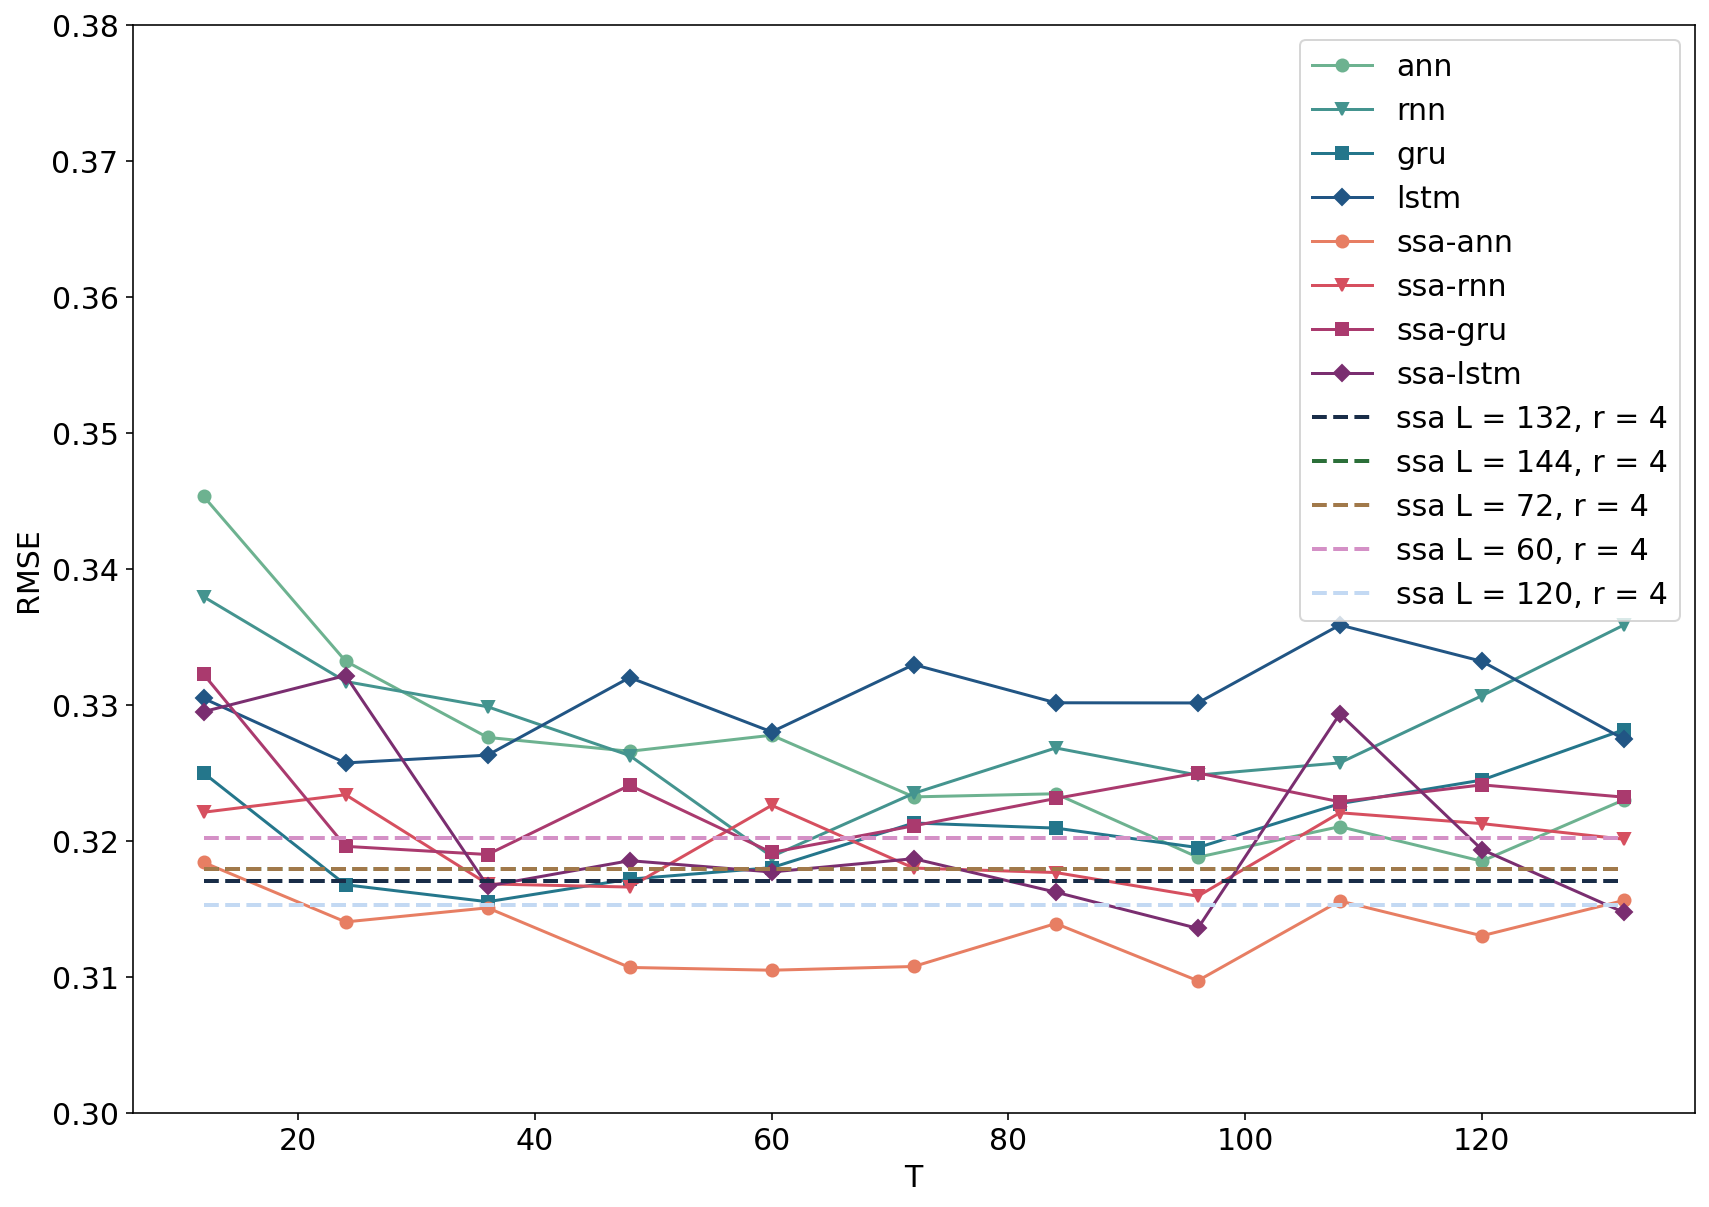
\includegraphics[width=0.9\linewidth, height=0.6\linewidth]{imgs/comp/edsine/N0.3/r6}}
	\caption{<<Сумма синусов с небольшим белым шумом>>. Ряд $\mathsf{X}_{650}$. Ошибки прогноза в зависимости от параметра $T$. $L = 175, \; r = 6$.}
	\label{edsin0.3r_r6}
\end{figure}

\subsubsection{Отображение прогнозов}
\label{edsine0.3r_res}

На графиках \multiref{edsin0.3r_r2_res_ann}{edsin0.3r_r6_res_ann} (больше графиков в приложении \ref{aedsine0.3r_res}) представлены результаты прогнозирования методами. Из-за маленького шума все прогнозы похожи друг на друга.

\begin{figure}[H]
	\captionsetup{justification=centering}
	\center{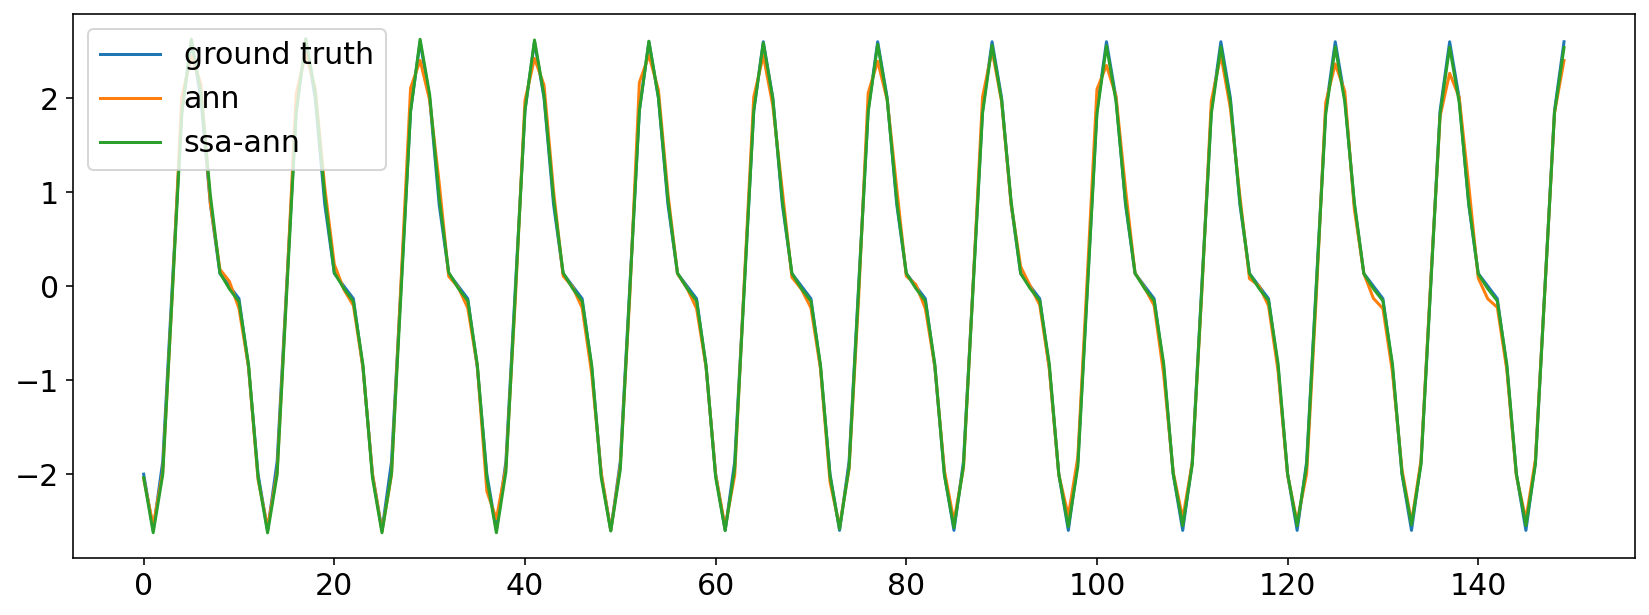
\includegraphics[width=0.9\linewidth]{imgs/comp/edsine/N0.3/edsin0.3r_r2_res_ann}}
	\caption{<<Сумма синусов с небольшим белым шумом>>. Ряд $\mathsf{X}_{650}$. Прогноз результатов для ANN и SSA-ANN. $r = 2$}
	\label{edsin0.3r_r2_res_ann}
\end{figure}

\begin{figure}[H]
	\captionsetup{justification=centering}
	\center{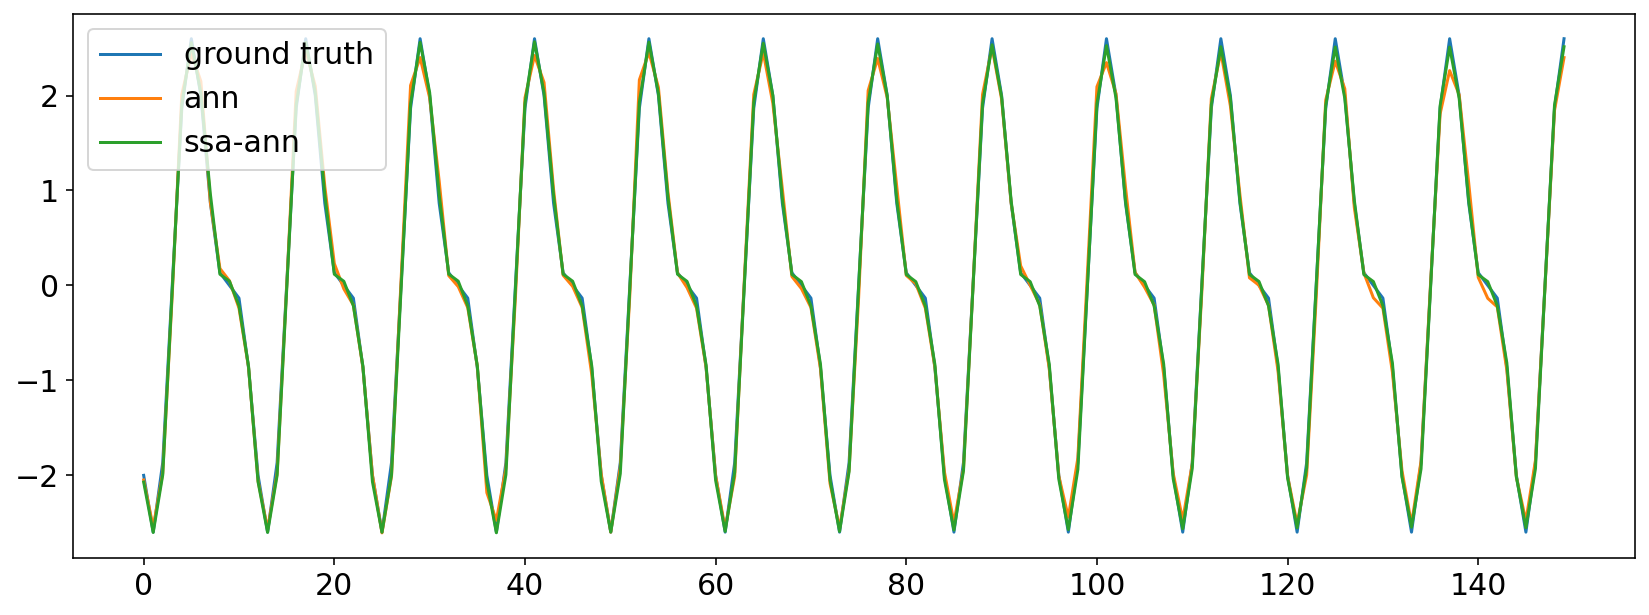
\includegraphics[width=0.9\linewidth]{imgs/comp/edsine/N0.3/edsin0.3r_r4_res_ann}}
	\caption{<<Сумма синусов с небольшим белым шумом>>. Ряд $\mathsf{X}_{650}$. Прогноз результатов для ANN и SSA-ANN. $r = 4$}
	\label{edsin0.3r_r4_res_ann}
\end{figure}

\begin{figure}[H]
	\captionsetup{justification=centering}
	\center{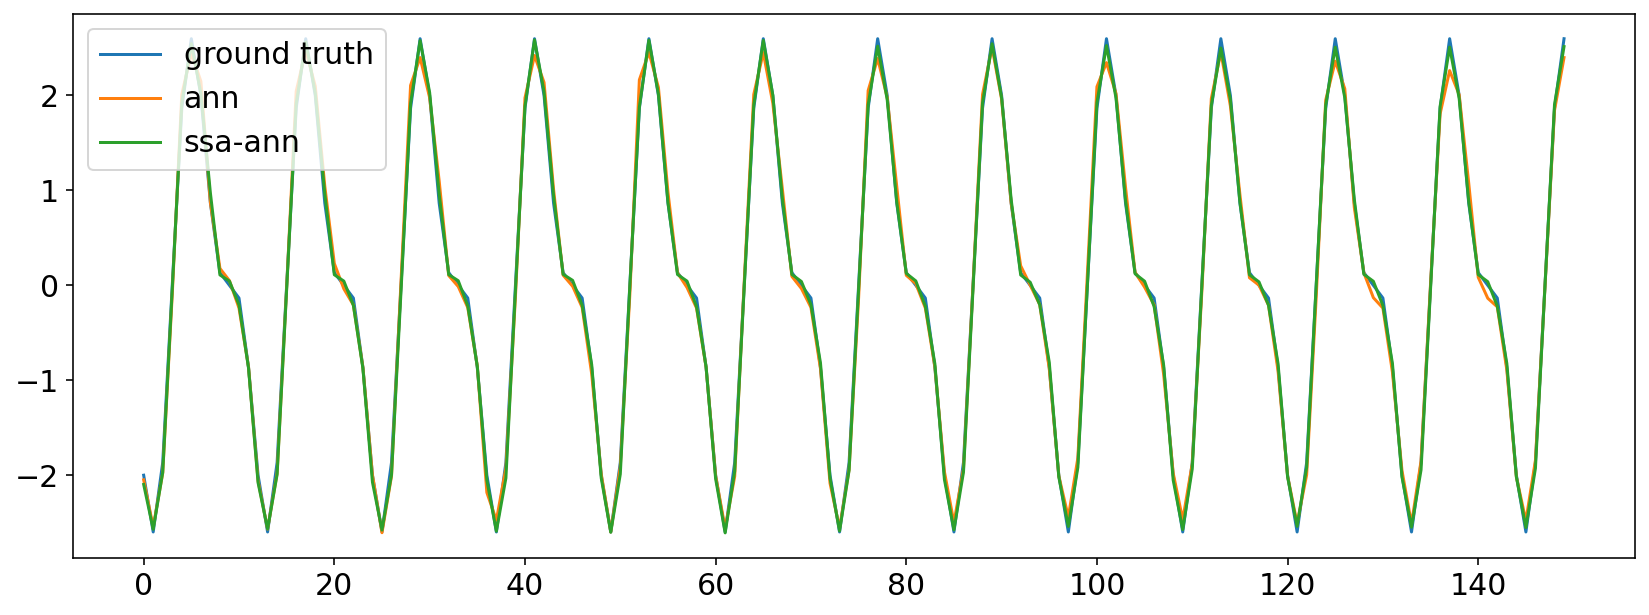
\includegraphics[width=0.9\linewidth]{imgs/comp/edsine/N0.3/edsin0.3r_r6_res_ann}}
	\caption{<<Сумма синусов с небольшим белым шумом>>. Ряд $\mathsf{X}_{650}$. Прогноз результатов для ANN и SSA-ANN. $r = 6$}
	\label{edsin0.3r_r6_res_ann}
\end{figure}

\subsubsection{Проверка устойчивости}
\label{edsine0.3r_rob}
Чтобы исключить случайность в полученных результатах, проведем сравнение для разных начальных весов методов. Зафиксируем новую сетку для параметра $T = \{12, 84\}$. Сетка для параметра $h$ останется прежней. Будем получать каждый результат по 7 раз, инициализируя метод с новыми весами. Полученные результаты отображены на рисунках \multiref{edsine0.3r2.12}{edsine0.3r6.84} в приложении \ref{aedsine0.3r_rob}. На них подтверждается, выводы сделанные ранее. Заключаем, что полученные результаты устойчивые.

\subsubsection{Выводы}

На ряде $\mathsf{X}_{650}$ было продемонстрировано сравнение обычных и гибридных методов, и метода SSA. Из полученных результатов и таблицы \ref{tedsineN0.3r} (таблица является аналогичной таблице \ref{tedsiner}) можем сделать выводы, что полученные результаты аналогичны результатам, полученным в разделе \ref{edsinr}. Из таблицы видно, что разница между параметрами $r$ не велика. Негибридные методы проигрывают гибридным в точности, но не сильно.
Если сравнивать средние значения, то видно, что ошибка прогноза по SSA примерно равна ошибке гибридных методов и они вместе выигрывают у негибридных нейронных сетей.

Таблица~\ref{bigtable} показывает, что из негибридных методов немного получше работает GRU. Все значения ошибок гибридных методов похожи, лучший результат достигает гибридный метод SSA-ANN.

\begin{table}[H]
	\captionsetup{justification=centering}
	\caption{<<Сумма синусов с небольшим белым шумом>>. Ряд $\mathsf{X}_{650}$. Усредненные и лучшие результаты прогнозов по RMSE.}
	\begin{center}
		\begin{tabular}{ccccc}
			\toprule
			{ssa-params} &  b-nn &  m-nn &  b-ssa &  m-ssa \\
			\midrule
			-          & 0.308 & 0.325 &  0.315 &  0.316 \\
			$ L = 175, \; r = 2$         & 0.307 & 0.313 &  0.315 &  0.316 \\
			$ L = 175, \; r = 4$         & 0.305 & 0.314 &  0.315 &  0.316 \\
			$ L = 175, \; r = 6$        & 0.304 & 0.316 &  0.315 &  0.316 \\
			\bottomrule
		\end{tabular}
	\end{center}
	\label{tedsineN0.3r}
\end{table}

\subsection{Влияние длины ряда}
\label{edsinlen}
Поставим задачу сравнить обычные и гибридные методы на временных рядах разной длины. Будем проводить сравнение на рядах $\mathsf{Z}_{650},\; \mathsf{Z}_{1500}$. В ходе эксперимента хотим выяснить, как длина ряда влияет на точность предсказаний.

\subsubsection{Прогноз по SSA}
Сравним точность прогнозирования методом SSA при разных параметрах $r$. Для ряда $\mathsf{Z}_{650}$ воспользуемся полученными результатами из раздела \ref{edsinr}. Для ряда $\mathsf{Z}_{1500}$ зададим следующую сетку параметров $L = \{12, 48, \ldots, 375\}$, $r = \{2, 4, 6\}$. Посмотрим на результаты на рисунке \ref{edsinlen_ssa_forecast}. На графике видно, что наилучшие результаты достигаются при $r = 4$, худшие результаты достигаются при $r = 2$. $r = 6$ дает неплохие результаты. Также заметим, что ошибка сильно упала по сравнению с рядом $\mathsf{Z}_{650}$ (рис. \ref{edsinr_ssa_forecast}). Также для ряда $\mathsf{Z}_{650}$  наихудшие результаты показывал параметр $r = 6$, для $\mathsf{Z}_{1500}$ наоборот. Это объяснимо тем, что при росте длины ряда, влияние шума, становится меньше. Алгоритму SSA становится проще выделить сигнал.

\begin{figure}[H]
	\captionsetup{justification=centering}
	\center{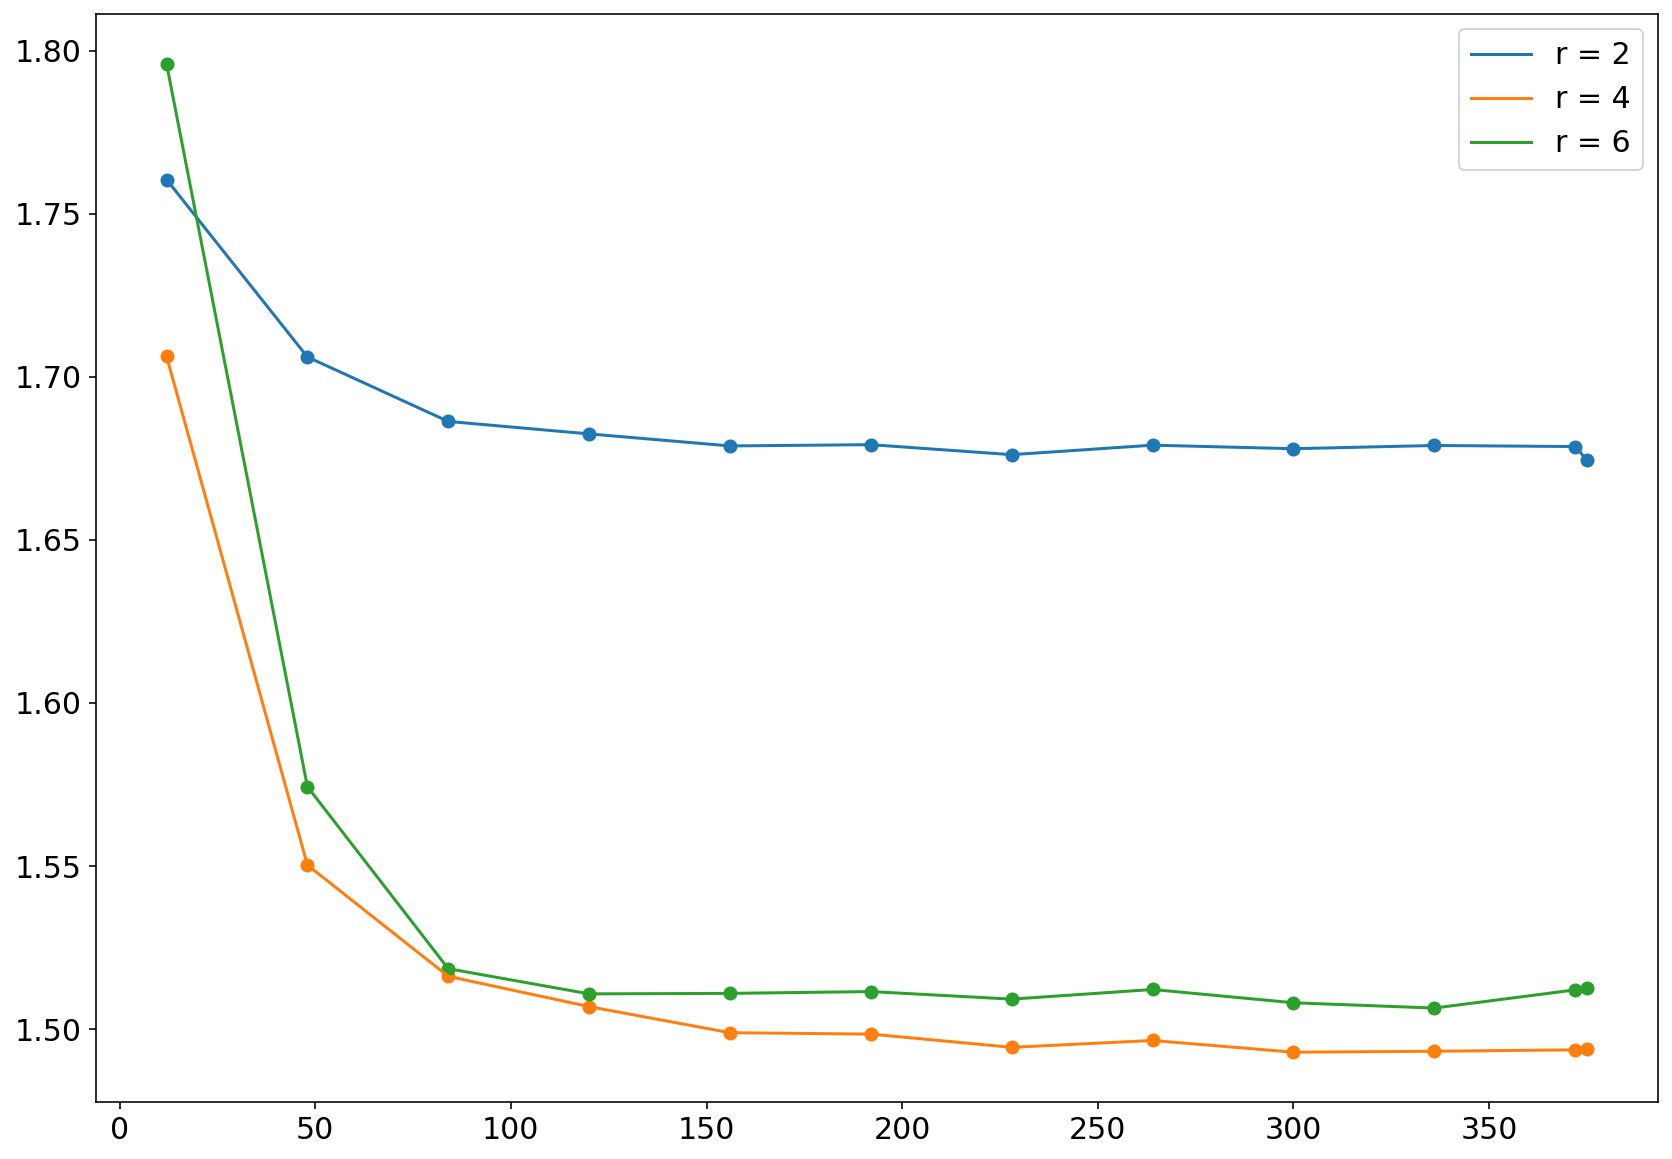
\includegraphics[width=0.9\linewidth]{imgs/comp/edsine/len/ssa_comp}}
	\caption{<<Сумма синусов с белым шумом>>. Ряд $\mathsf{Z}_{1500}$. RMSE прогноз на валидационной части.}
	\label{edsinlen_ssa_forecast}
\end{figure}

На основе полученных результаты зафиксируем наилучшие параметры SSA. Для ряда $\mathsf{Z}_{650}$ параметры $L = 175$ и $r = 4$, для ряда $\mathsf{Z}_{1500}$ параметры $L = 375$ и $r = 4$. Далее в гибридных моделях и прогнозе SSA будем использовать эти параметры.

\subsubsection{Восстановление SSA}
Посмотрим на то, как метод SSA восстановил тренировочную выборку ряда $\mathsf{Z}_{1500}$ с выбранными ранее параметрами (рис. \ref{edsinlen_rec4}). На графике видно, что метод хорошо выделил сигнал, но в самом конце амплитуда начала уменьшаться. Результаты восстановление сигнала для $\mathsf{Z}_{650}$ были представлены ранее (рис. \ref{edsinr_rec4}).

\begin{figure}[H]
	\captionsetup{justification=centering}
	\center{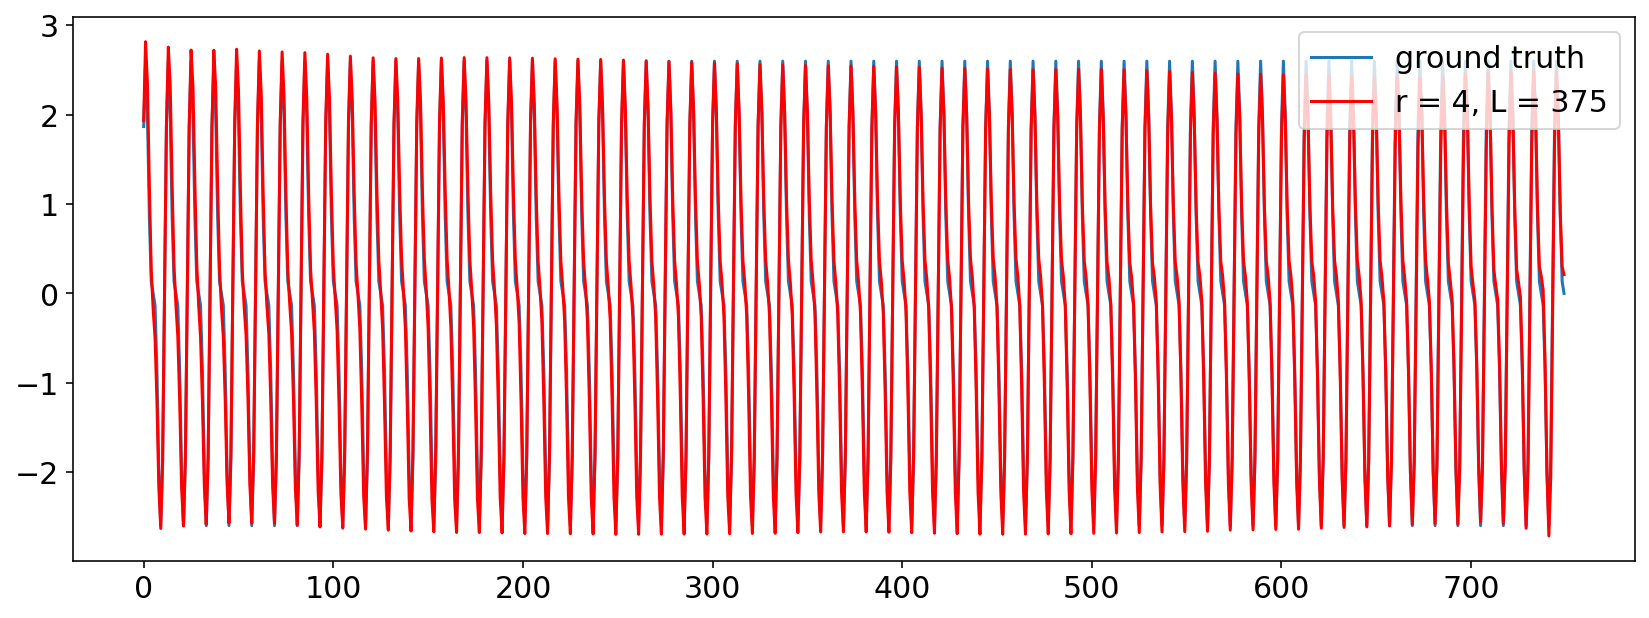
\includegraphics[width=0.9\linewidth]{imgs/comp/edsine/len/edsinerec4}}
	\caption{<<Сумма синусов с белым шумом>>. Ряд $\mathsf{Z}_{1500}$. Восстановление тренировочной выборки с помощью метода SSA. $r = 4$}
	\label{edsinlen_rec4}
\end{figure}

\subsubsection{Сравнение обычных и гибридных методов}

Для нейронных сетей зададим следующую сетку параметров: $T = \{12, 48, \ldots, 444 \}$, $h = \{10, 25, \ldots, 100 \}$. Для метода SSA в гибридных моделях возьмем пары параметров, выбранные выше.

На графиках \ref{edsinlen_r4} и \ref{edsinlen_r4.h}, представлены результаты сравнения для ряда $\mathsf{Z}_{1500}$. Результаты для ряда $\mathsf{Z}_{650}$ были продемонстрированны ранее (рис. \ref{edsinr_r4}). На графиках ниже, мы можем наблюдать превосходство гибридных методов. Но такое же превосходство мы наблюдали на графикe \ref{edsinr_r4} для ряда $\mathsf{Z}_{650}$ ранее.

\begin{figure}[H]
	\captionsetup{justification=centering}
	\center{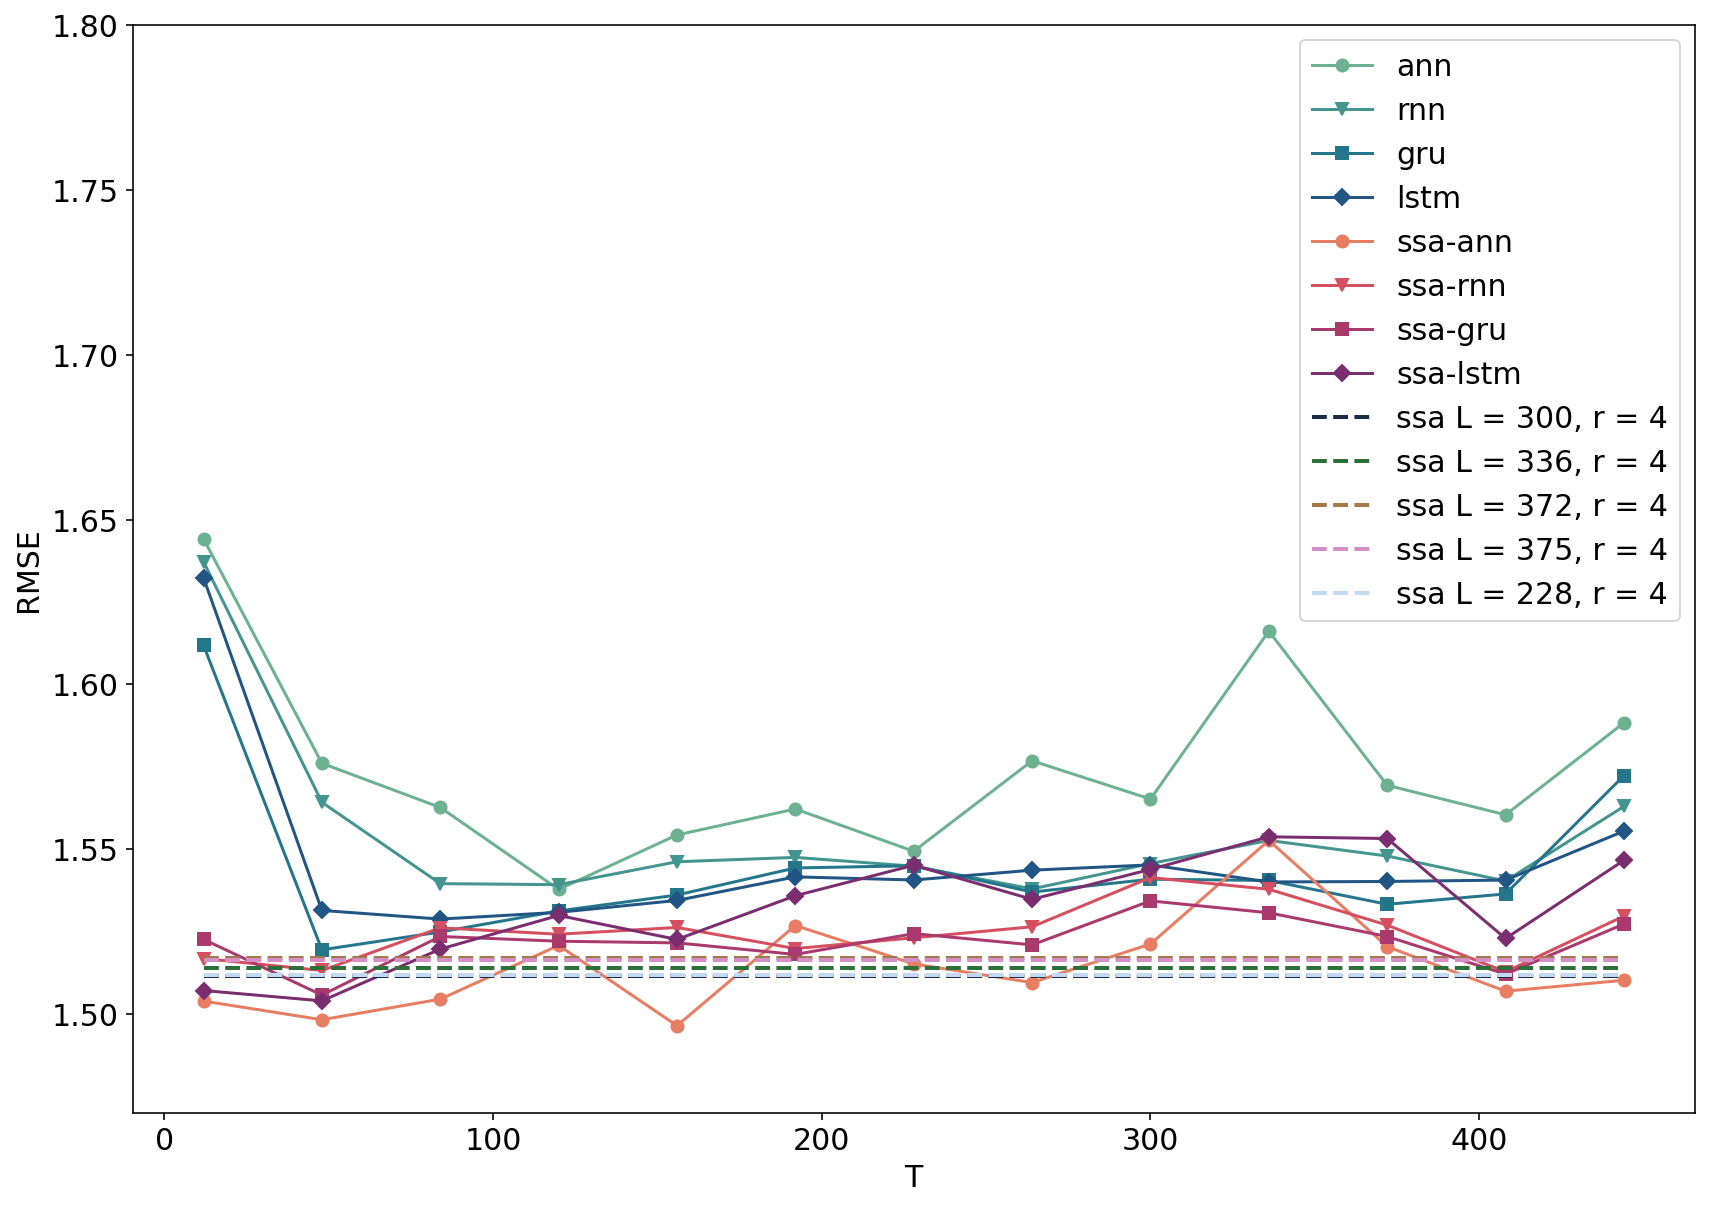
\includegraphics[width=0.9\linewidth, height=0.6\linewidth]{imgs/comp/edsine/len/r4}}
	\caption{<<Сумма синусов с белым шумом>>. Ряд $\mathsf{Z}_{1500}$. Ошибки прогноза в зависимости от параметра $T$. $L = 375, \; r = 4$.}
	\label{edsinlen_r4}
\end{figure}

\begin{figure}[H]
	\captionsetup{justification=centering}
	\center{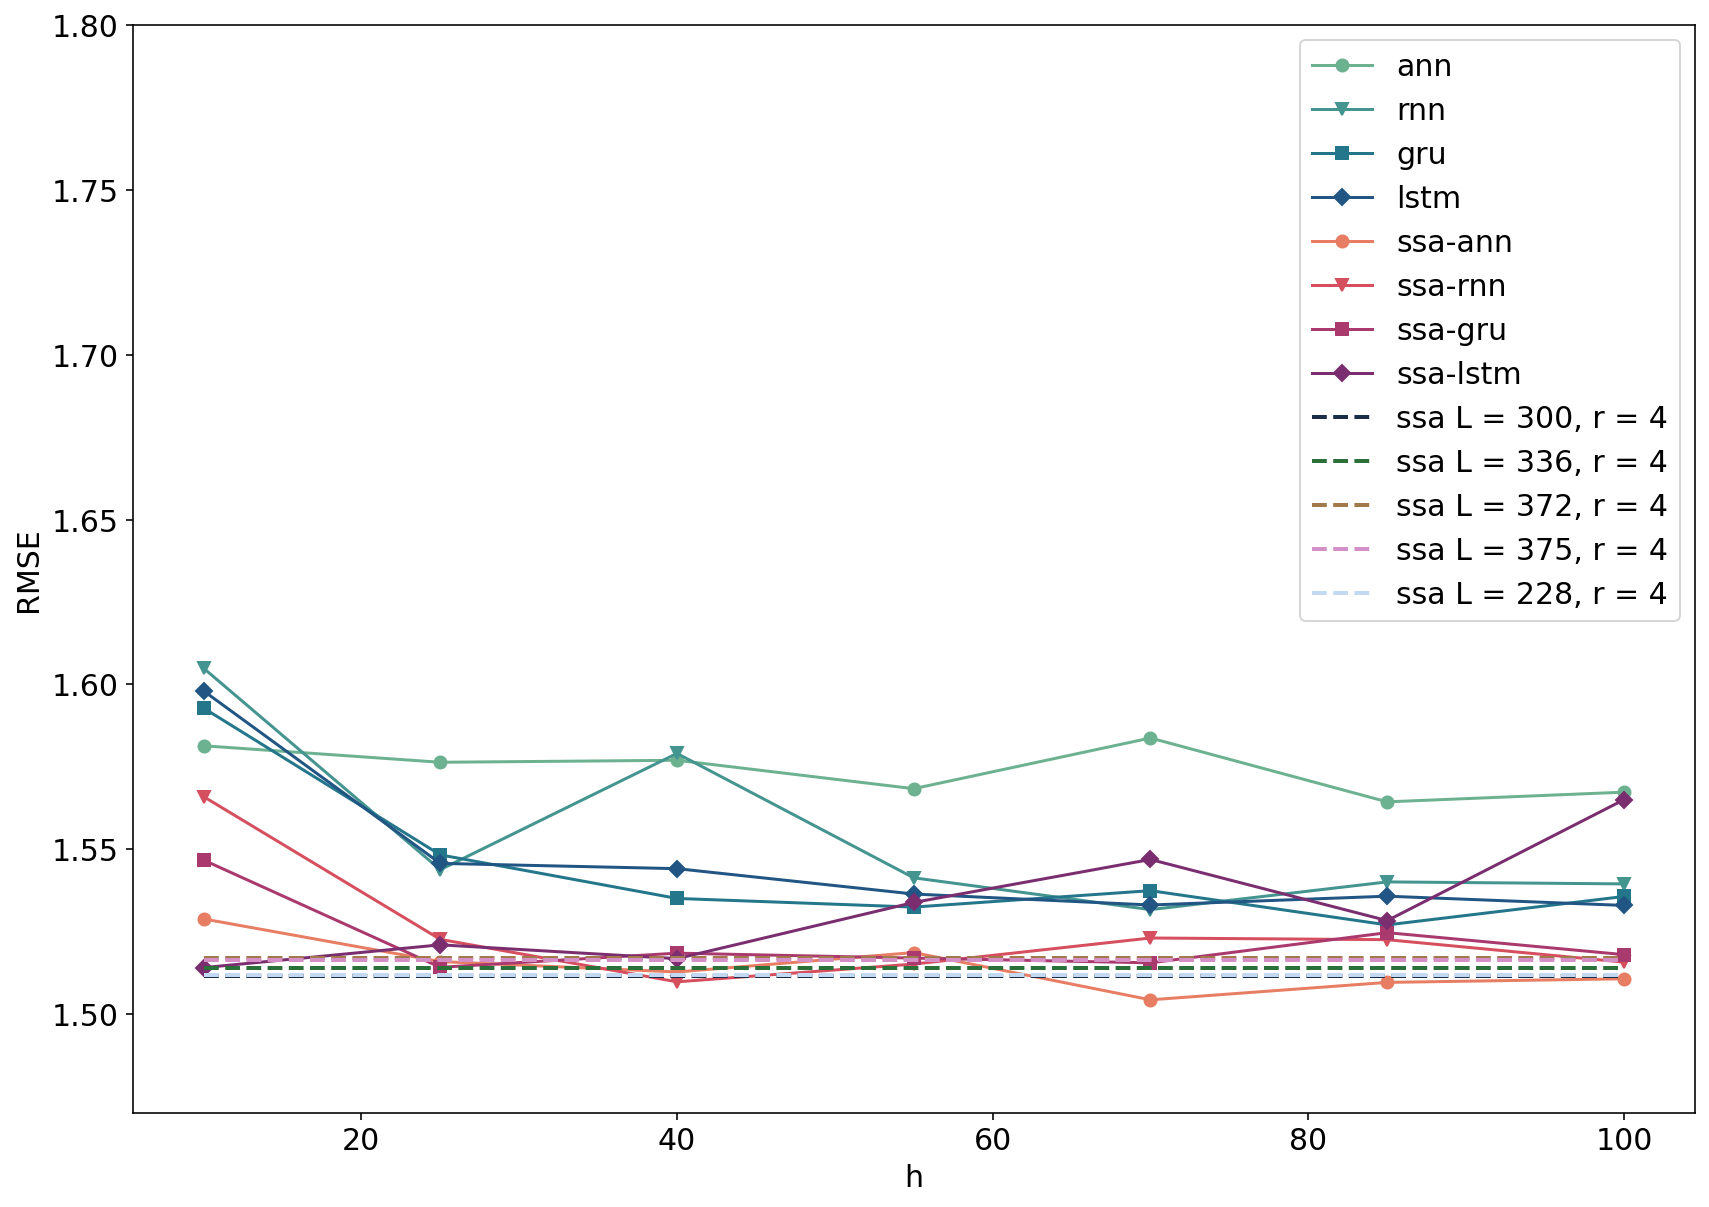
\includegraphics[width=0.9\linewidth, height=0.6\linewidth]{imgs/comp/edsine/len/r4.h}}
	\caption{<<Сумма синусов с белым шумом>>. Ряд $\mathsf{Z}_{1500}$. Ошибки прогноза в зависимости от параметра $h$. $L = 375, \; r = 4$.}
	\label{edsinlen_r4.h}
\end{figure}

\subsubsection{Отображение прогнозов}

Ниже на графиках представлены результаты прогнозирования методами для ряда $\mathsf{Z}_{1500}$. На графиках видно, что предсказания для гибридных методов больше напоминают сигнал ряда. Видно, что в прогноз обычных методов проникает шум.

\begin{figure}[H]
	\captionsetup{justification=centering}
	\center{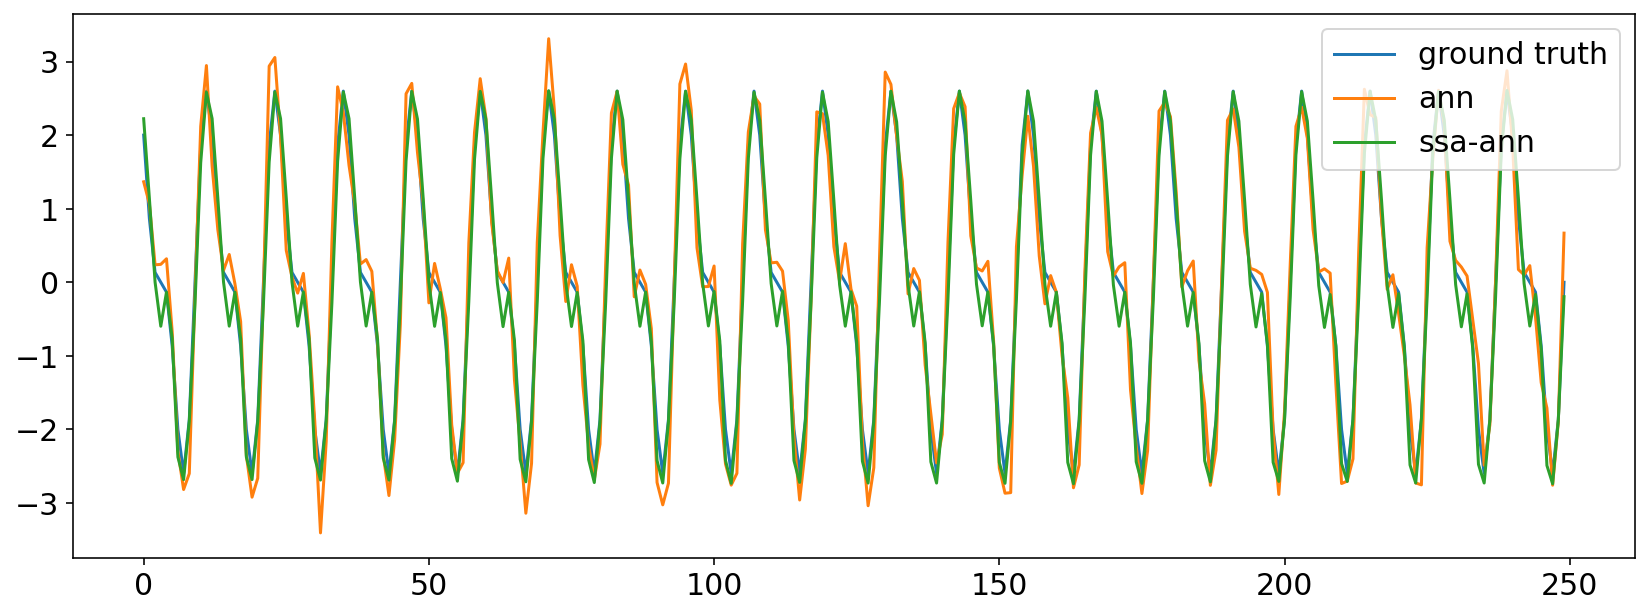
\includegraphics[width=0.9\linewidth]{imgs/comp/edsine/len/edsinlen_r4_res_ann}}
	\caption{<<Сумма синусов с белым шумом>>. Ряд $\mathsf{Z}_{1500}$. Прогноз для ANN и SSA-ANN. $r = 4$}
	\label{edsinlen_r4_res_ann}
\end{figure}

\begin{figure}[H]
	\captionsetup{justification=centering}
	\center{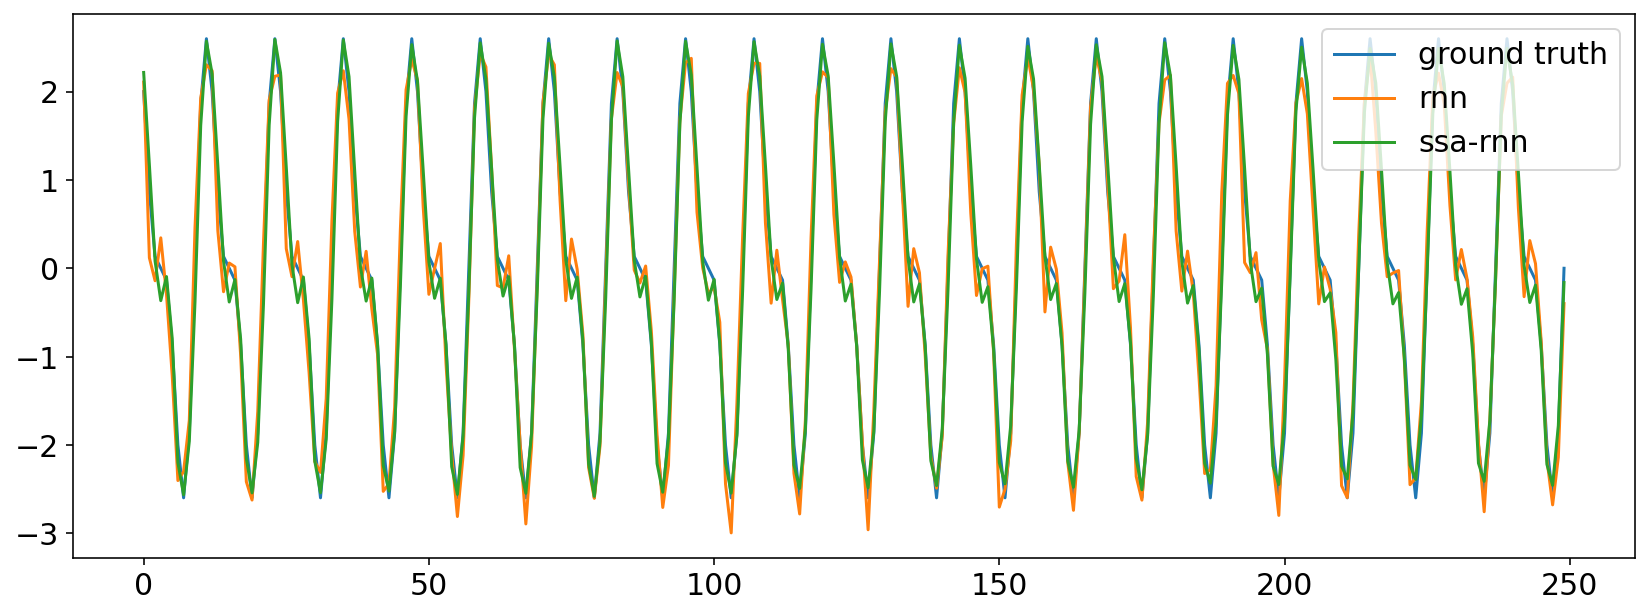
\includegraphics[width=0.9\linewidth]{imgs/comp/edsine/len/edsinlen_r4_res_rnn}}
	\caption{<<Сумма синусов с белым шумом>>. Ряд $\mathsf{Z}_{1500}$. Прогноз для RNN и SSA-RNN. $r = 4$}
	\label{edsinlen_r4_res_rnn}
\end{figure}

\begin{figure}[H]
	\captionsetup{justification=centering}
	\center{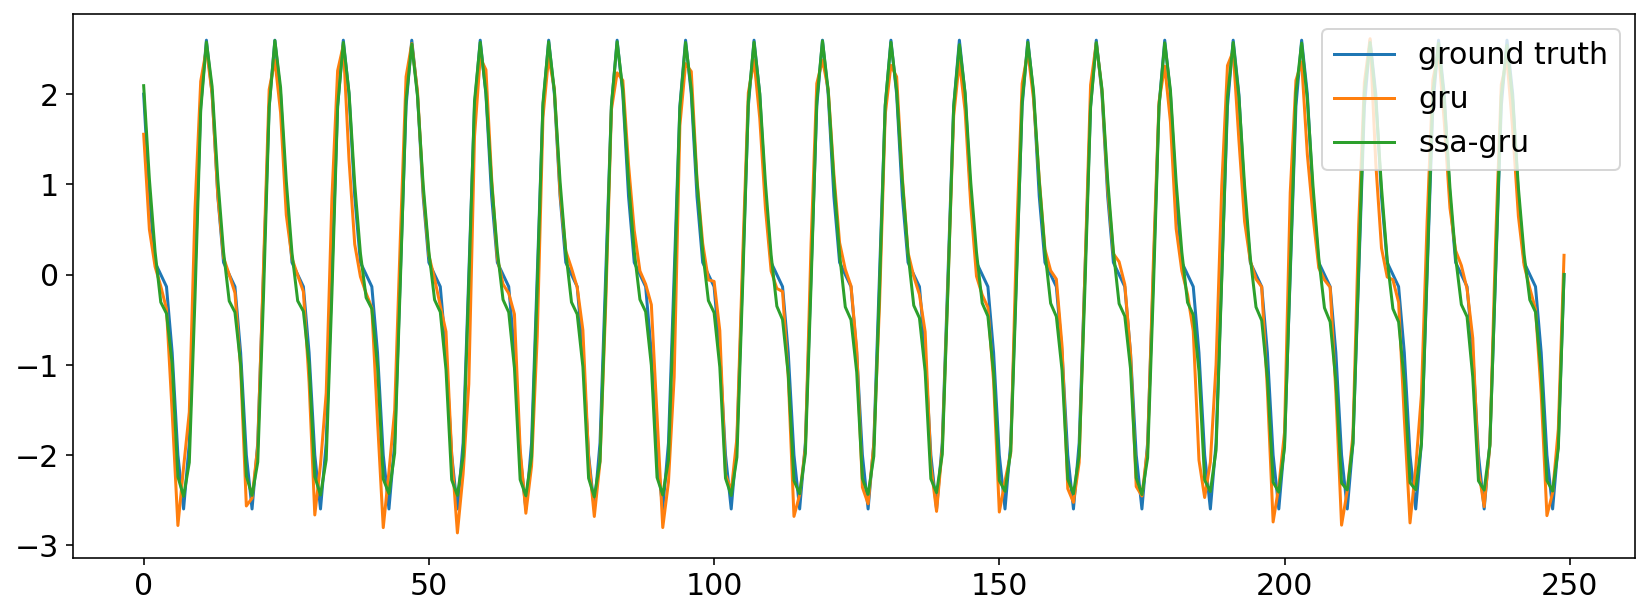
\includegraphics[width=0.9\linewidth]{imgs/comp/edsine/len/edsinlen_r4_res_gru}}
	\caption{<<Сумма синусов с белым шумом>>. Ряд $\mathsf{Z}_{1500}$. Прогноз для GRU и SSA-GRU. $r = 4$}
	\label{edsilen_r4_res_gru}
\end{figure}

\begin{figure}[H]
	\captionsetup{justification=centering}
	\center{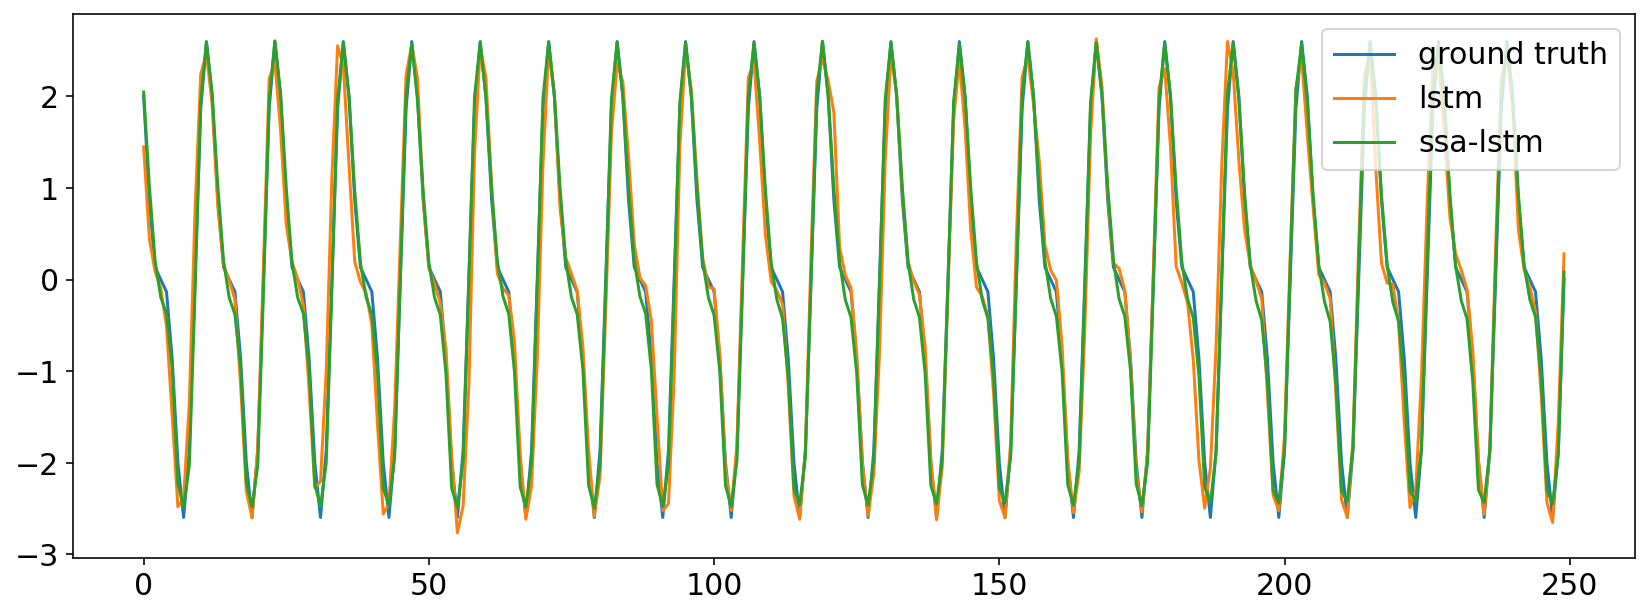
\includegraphics[width=0.9\linewidth]{imgs/comp/edsine/len/edsinlen_r4_res_lstm}}
	\caption{<<Сумма синусов с белым шумом>>. Ряд $\mathsf{Z}_{1500}$. Прогноз для LSTM и SSA-LSTM. $r = 4$}
	\label{edsinlen_r4_res_lstm}
\end{figure}

\subsubsection{Проверка устойчивости}
Чтобы исключить случайность в полученных результатах, проведем сравнение для разных начальных весов методов. Зафиксируем новую сетку для параметра $T = \{12, 156\}$. Сетка для параметра $h$ останется прежней. Будем получать каждый результат по 7 раз, инициализируя метод с новыми весами. Полученные результаты отображены на рисунках \multiref{edsinelen4.12}{edsinelen4.156}. На них подтверждается, выводы сделанные ранее. Заключаем, что полученные результаты устойчивые.

\begin{figure}[h]
	\captionsetup{justification=centering}
	\center{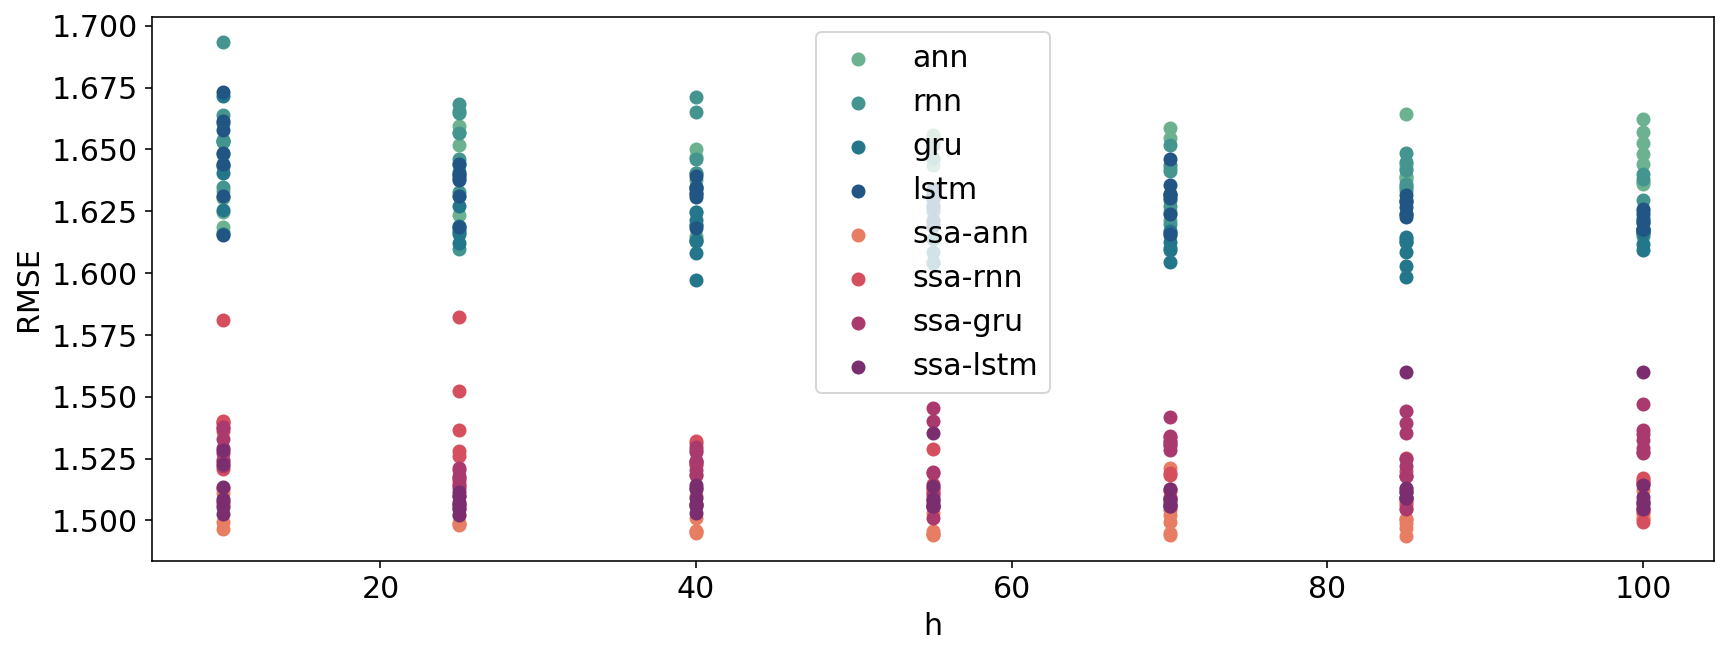
\includegraphics[width=0.9\linewidth]{imgs/comp/edsine/len/loopr4.12}}
	\caption{<<Сумма синусов с белым шумом>>. Ряд $\mathsf{Z}_{1500}$. Проверка устойчивости. $r = 4, \; L = 175$. $T = 12$.}
	\label{edsinelen4.12}
\end{figure}

\begin{figure}[h]
	\captionsetup{justification=centering}
	\center{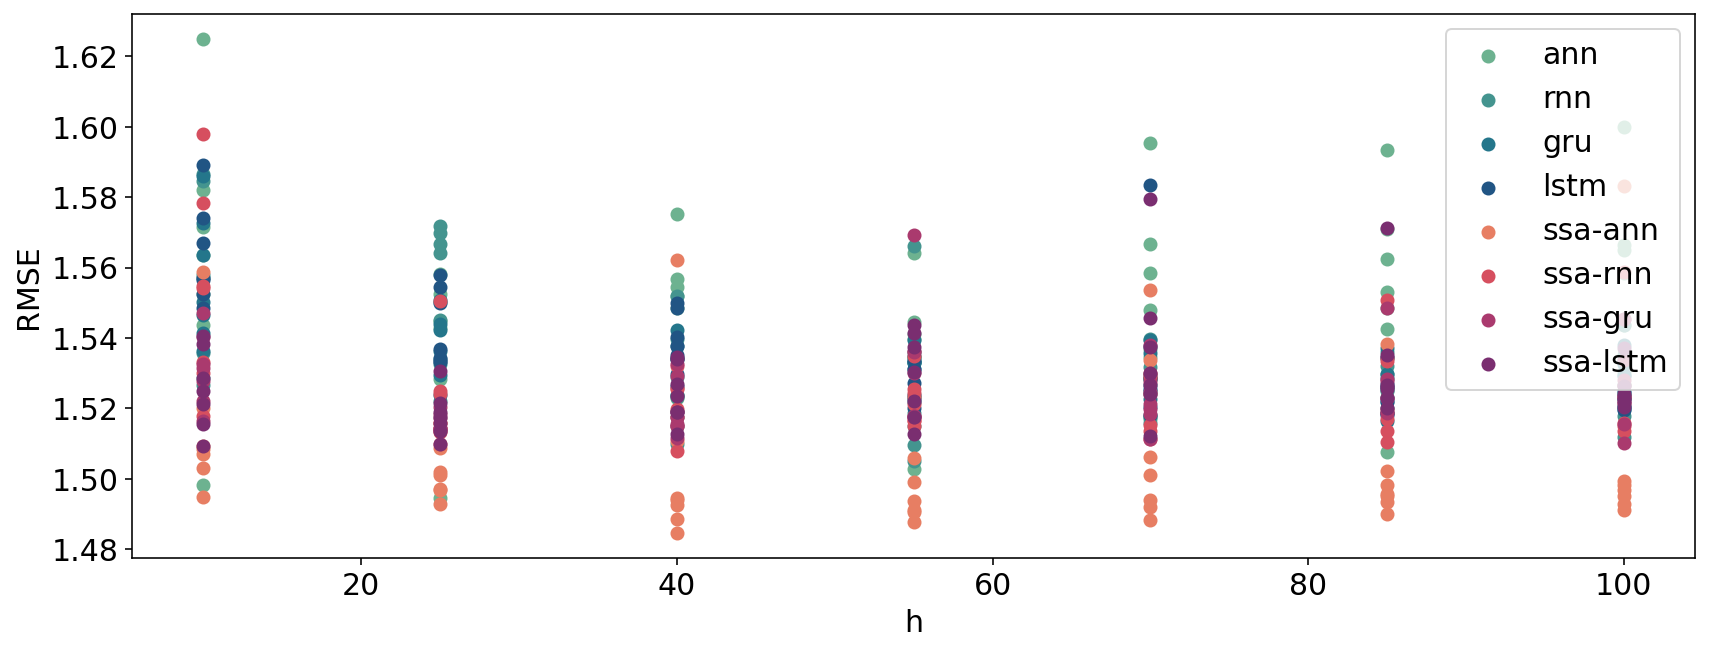
\includegraphics[width=0.9\linewidth]{imgs/comp/edsine/len/loopr4.156}}
	\caption{<<Сумма синусов с белым шумом>>. Ряд $\mathsf{Z}_{1500}$. Проверка устойчивости. $r = 4, \; L = 375$. $T = 156$.}
	\label{edsinelen4.156}
\end{figure}

\subsubsection{Выводы}
Из полученных результатов и таблицы \ref{tedsinelen} (таблица является аналогичной таблице \ref{tedsiner}) можно сделать выводы, что увеличение длины ряда позволяет улучшить прогноз нейронными сетями, что ведет также к улучшению точности прогнозировании гибридными методами. Также увеличение длины ряда позволяет лучше выделить сигнал, что также приводит к улучшению точности гибридных методов. Из полученных результатов можем заключить, что увеличение длины ряда положительно сказывается на точности прогнозирования обычных и гибридных методов, особенно для метода SSA. Из таблицы видно, что средняя ошибка прогноза методом SSA, меньше, чем средняя ошибка для методов с нейронными сетями.

Для ряда $\mathsf{Z}_{1500}$ наилучшую точность среднюю показали метод SSA и гибридные методы. Негибридные методы показывают результаты немного хуже.

Таблица~\ref{bigtable} показывает, что для ряда $\mathsf{Z}_{1500}$ из негибридных методов хорошо работают GRU и LSTM. Лучший результат достигает гибридный метод SSA-ANN. Лучшие результаты для ряда $\mathsf{Z}_{650}$ можно посмотреть в <<Выводах>> раздела \ref{edsinr}.

\begin{table}[h]
	\captionsetup{justification=centering}
	\caption{<<Сумма синусов с белым шумом>>. Ряды $\mathsf{Z}_{650}$ и $\mathsf{Z}_{1500}$. Усредненные и лучшие результаты прогнозов по RMSE.}
	\begin{center}
		\begin{tabular}{cccccc}
			\toprule
			ts &  ssa-params  &  b-nn &  m-nn &  b-ssa &  m-ssa \\
			\midrule
			$\mathsf{Z}_{650}$ & - & 1.547 & 1.635 &  1.581 &  1.586 \\
			& $L = 175, \; r = 4$ & 1.532 & 1.575 &  1.581 &  1.586 \\
			$\mathsf{Z}_{1500}$ & - & 1.504 & 1.550 &  1.511 &  1.512 \\
			& $L = 375, \; r = 4$ & 1.484 & 1.520 &  1.511 &  1.512 \\
			\bottomrule
		\end{tabular}
	\end{center}
	\label{tedsinelen}
\end{table}

\clearpage

\section{Сумма двух синусов с красным шумом. Ряд с трудно отделимым сигналом}
\label{ser}
Рассмотрим следующий ряд $\mathsf{V}_{650}$ (рис. \ref{ser_graph}), состоящий из элементов: $$ z_i = \big(\sin(2 \pi \dfrac{i}{6} ) + 2 \cdot \sin(2 \pi \dfrac{i}{12} ) \big) + \xi_i, $$ где $\xi_i = \xi_{i-1} + \sigma \varepsilon_{i}$, $\sigma = 1.2$, $\varepsilon_i \sim \mathrm{N}(0, 1)$.

Сигнал данного ряда идентичен сигналу ряда из раздела \ref{edsine}. Отличие состоит в шуме, он --- красный, что делает выделение сигнала сложной задачей, так как он сильно смешивается с шумом.  Это можно увидеть на периодограмме (рис. \ref{ser_pgram}).

Другим важным отличием этого примера является то, что красный шум в отличие от белого шума допускает осмысленный прогноз сам по себе. Поэтому можно ставить две разные задачи --- прогноз сигнала и прогноз ряда целиком (для белого шума эти задачи не различаются).

Из формулы видно, что сигнал стоит из двух синусов с периодами $12$ и $6$, общий период  ряда $12$. В дальнейшем будем выбирать сетки для параметров $T$ и $L$ кратные $12$. Исходя из раздела \ref{edsine}, можно зафиксировать аналитически верными параметры $L = 175, \; r = 4$ для прогноза сигнала, но для так как из-за красного шума сигнал сложно выделить, то возможно данная пара будет не оптимальной даже для прогноза сигнала. Далее в разделе сравним разные параметры для метода SSA, выберем те, которые дают хорошую точность, а также не слишком хорошо аппроксимируют ряд оценкой сигнала, иначе гибридные методы будут не отличаться от негибридных. Выбирая лучшие пары, будем ориентироваться на прогноз всего ряда.

\begin{figure}[H]
	\center{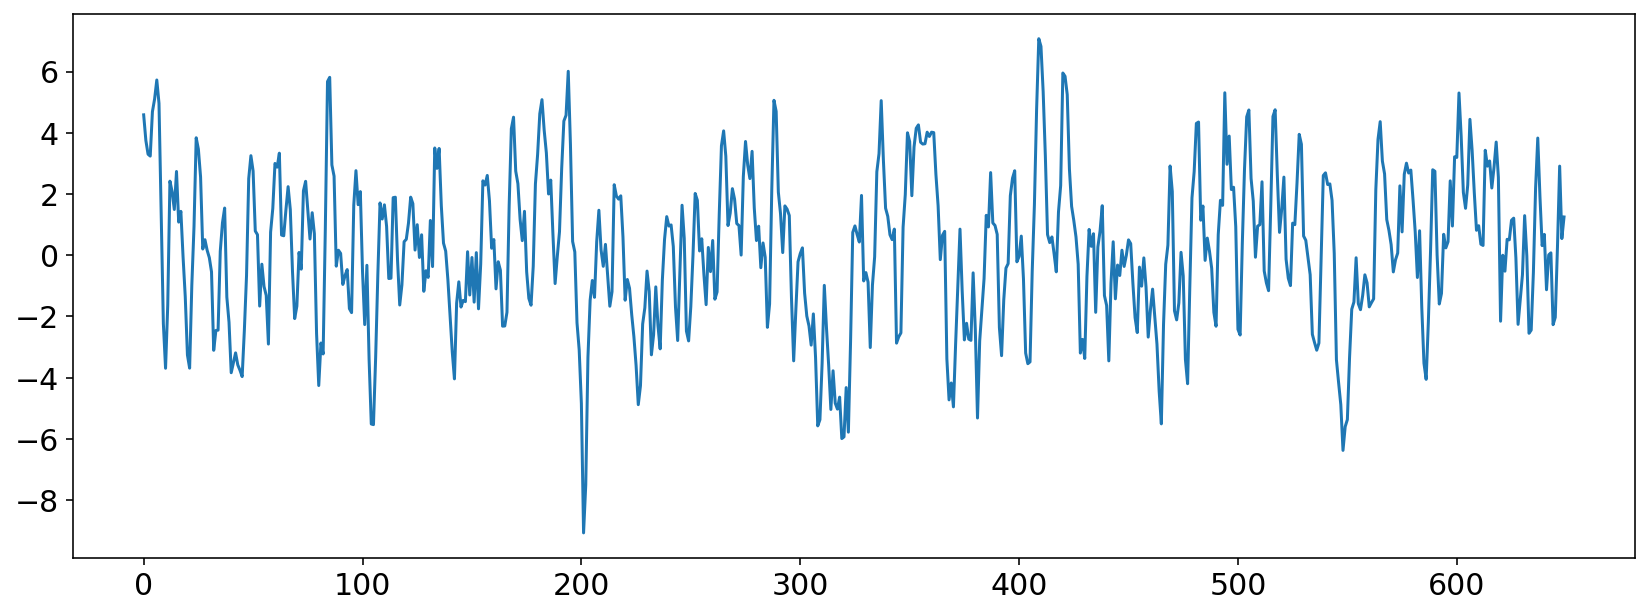
\includegraphics[width=0.9\linewidth]{imgs/ts/ser/ser}}
	\caption{Ряд суммы синусов с красным шумом $\mathsf{V}_{650}$.}
	\label{ser_graph}
\end{figure}

\begin{figure}[H]
	\center{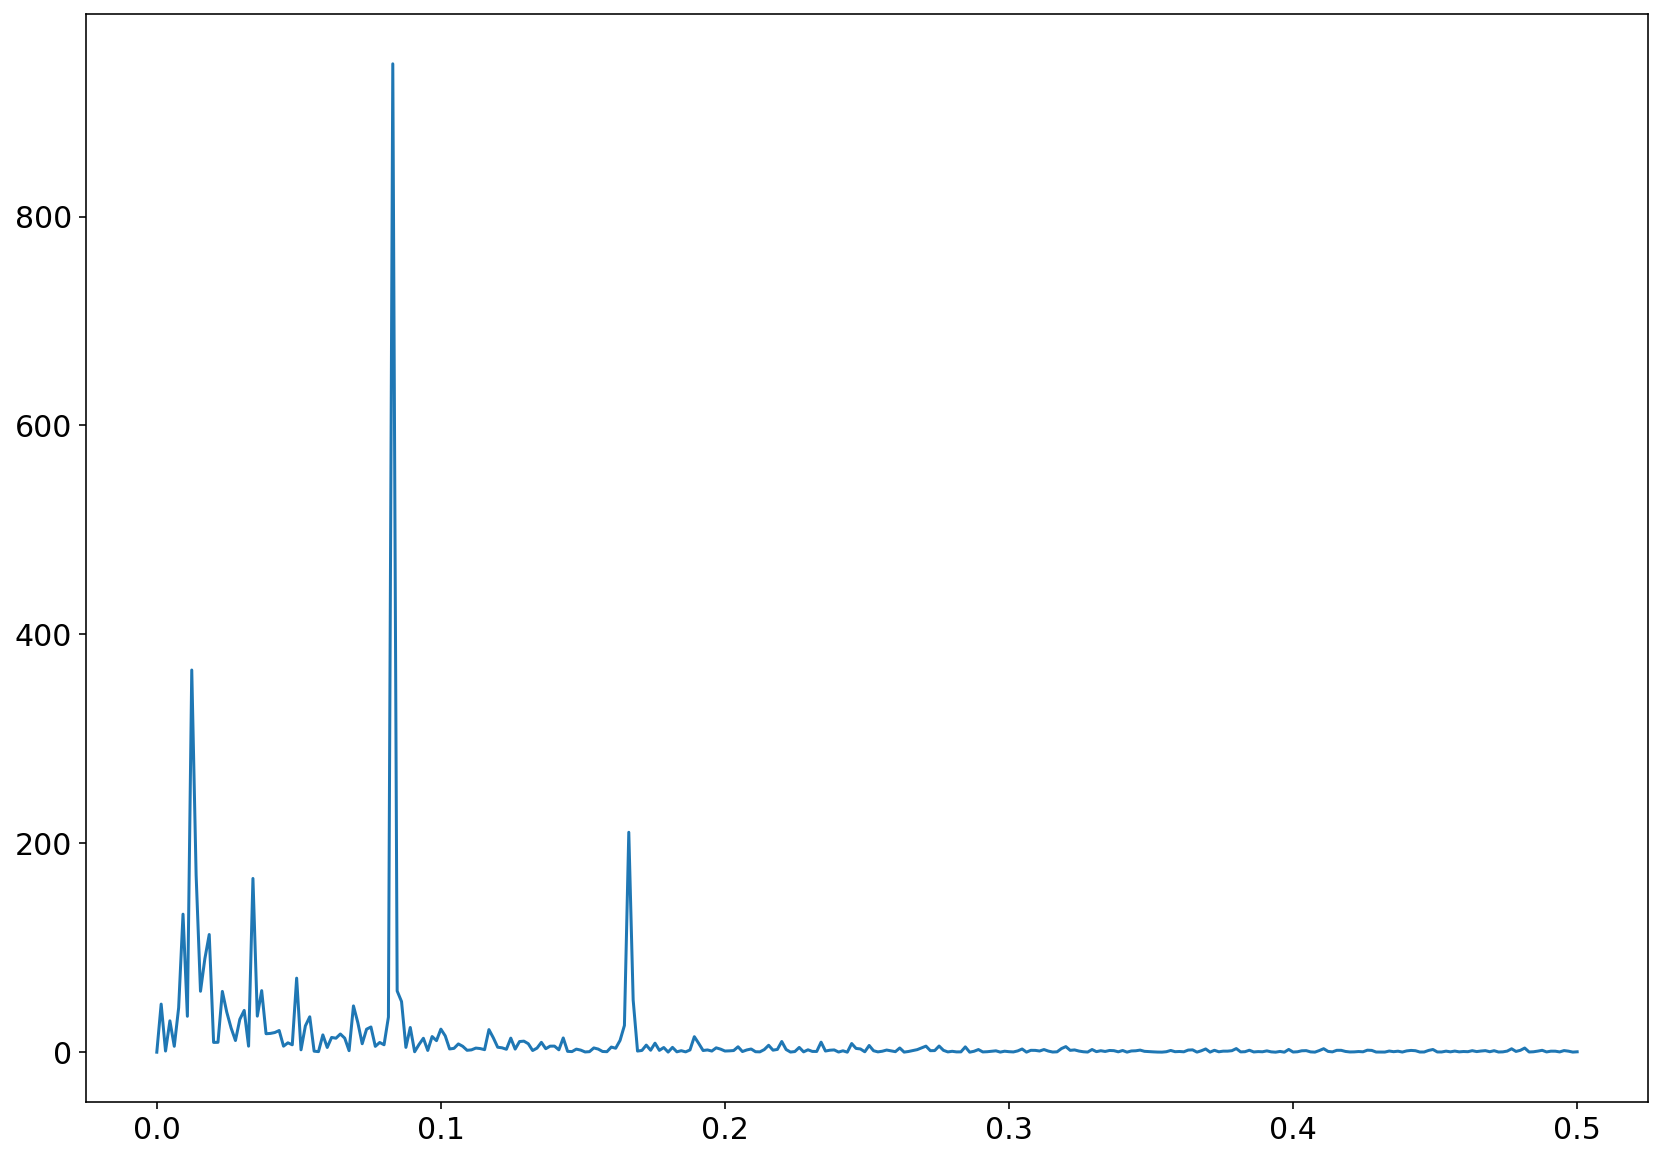
\includegraphics[width=0.9\linewidth]{imgs/ts/ser/ser_pgram}}
	\caption{Периодограмма ряда $\mathsf{V}_{650}$.}
	\label{ser_pgram}
\end{figure}

\subsection{Сравнение прогнозов, полученных с помощью метода SSA, обычных и гибридных методов}
\label{serr}

Поставим задачу сравнить обычные, гибридные методы и метод SSA на ряде $\mathsf{V}_{650}$. Проводить сравнение будем по методу, описанному в разделе \ref{comp_tactic}. В ходе эксперимента хотим посмотреть как поведут себя гибридные методы, столкнувшись с рядом, в котором сложно корректно выделить сигнал. Будем проводить сравнение для аналитически верной пары $L = 175, \; r = 4$, а также для оптимальной пары, которую выделим на этапе сравнения параметров SSA прогноза.

\subsubsection{Прогноз по SSA}
Сравним точность прогнозирования методом SSA при разных параметрах. Зададим следующую сетку параметров $L = \{ 12, 24, \ldots, 175 \}$, $r = \{ 2, 4, 6, 8, 10, 12, 16 \}$.

Посмотрим на результаты на рисунке \ref{serr_ssa_forecast}. На графике видно, что чем меньше $r$, тем выше ошибка. Для $r \geqslant 8$ разница между ошибками не такая большая, и результаты начинают смешиваться. Из графика видно, что $r = 2$ дает результаты сильно хуже, чем остальные варианты. Также заметим, что ошибка для аналитическо верной пары растет с ростом $L$. Пока что сложно выделить, лучшую пару параметров. Прежде чем сделать это, посмотрим как каждая пара параметров выделяет сигнал на тренировочной выборки.

\begin{figure}[H]
	\captionsetup{justification=centering}
	\center{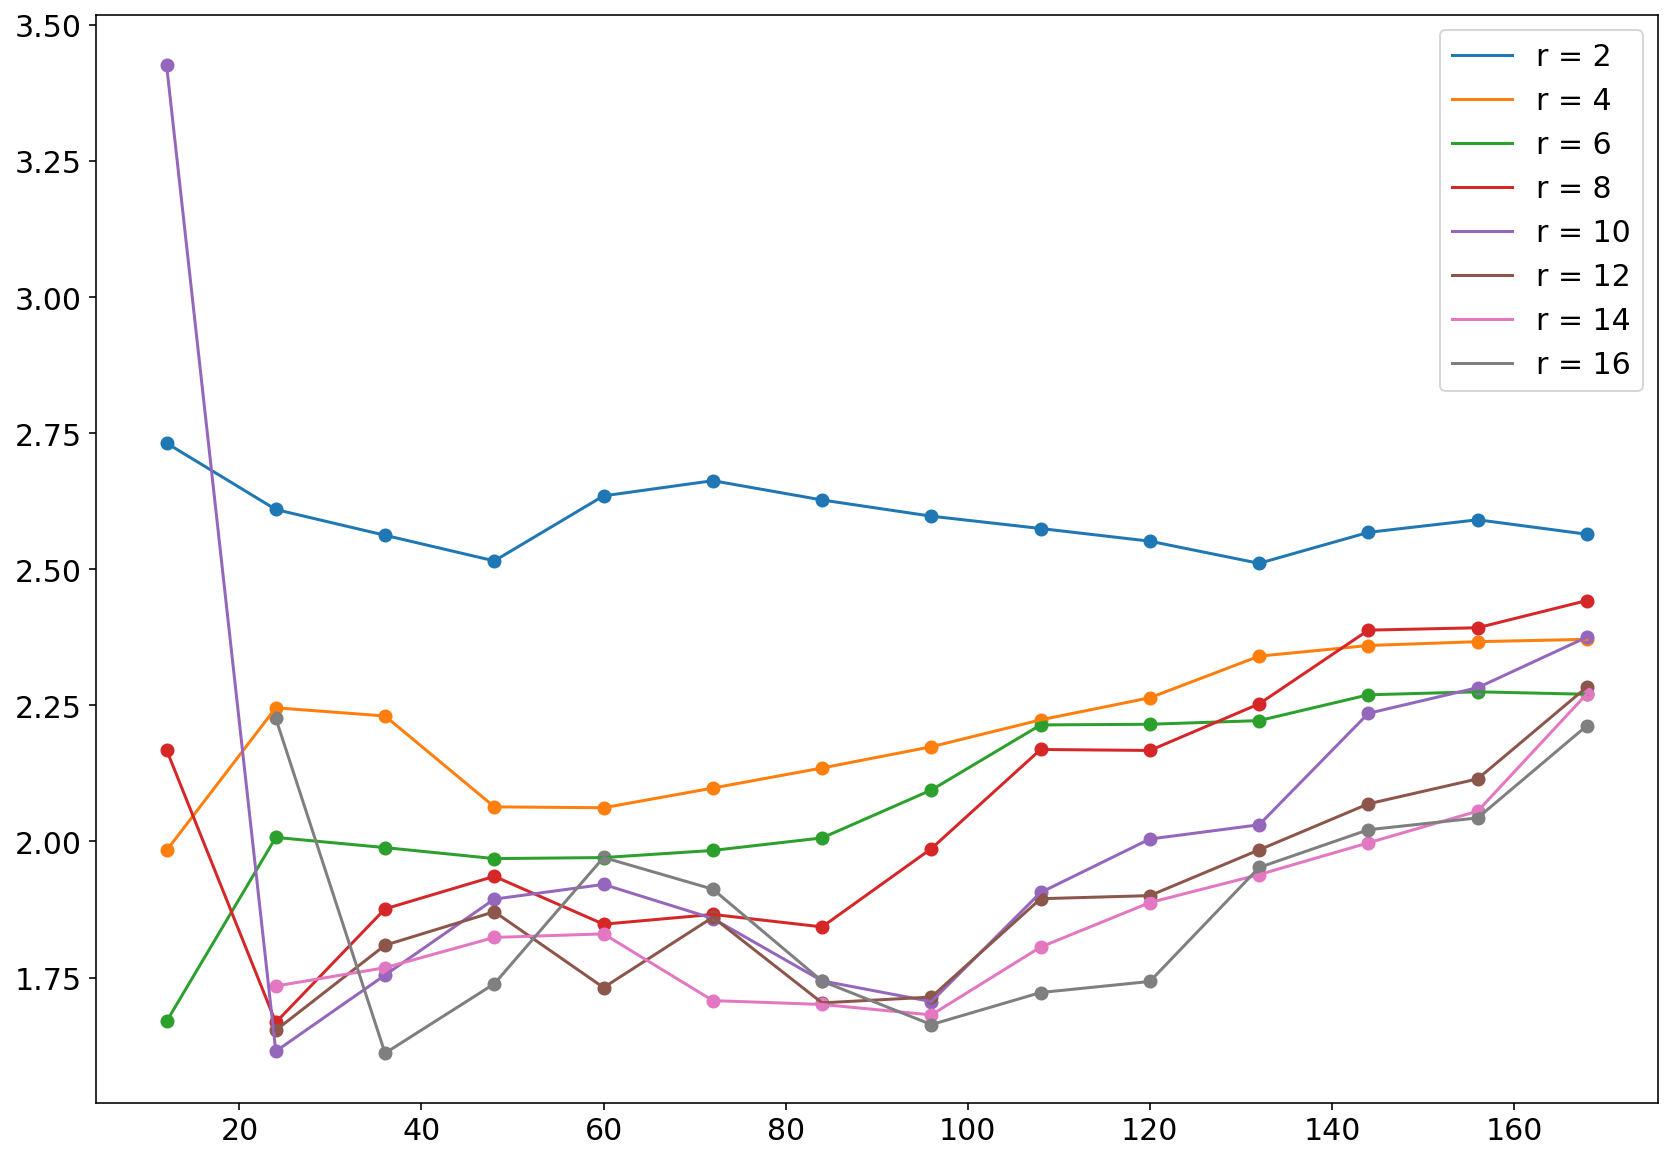
\includegraphics[width=0.9\linewidth]{imgs/comp/ser/ssa_comp}}
	\caption{<<Сумма синусов с красным шумом>>. Ряд $\mathsf{V}_{650}$. RMSE прогноз на валидационной части.}
	\label{serr_ssa_forecast}
\end{figure}


\subsubsection{Восстановление SSA}

Посмотрим как SSA восстанавливает тренировочную выборку. На графике показана зависимость ошибки восстановления тренировочной выборки от параметра $L$. Сетку для параметров оставим такую же. На графике \ref{serr_ssa_reconstruct} представлены результаты. Видно, что наилучшие результаты показывает пара $r = 2, \; L = 175$. Для других $r$ ситуация выглядит похоже. Для сравнения возьмем пару $r = 6, \; L = 175$ и аналитически верную пару $r = 4, \; L = 175$. Также возьмем две пары $r = 16, \; L = 36$ и $r = 14, \; L = 84$, как показывающие низкую ошибку на графике \ref{serr_ssa_forecast}. Для выбранных пар покажем как метод SSA восстанавливает сигнал.

\begin{figure}[H]
	\captionsetup{justification=centering}
	\center{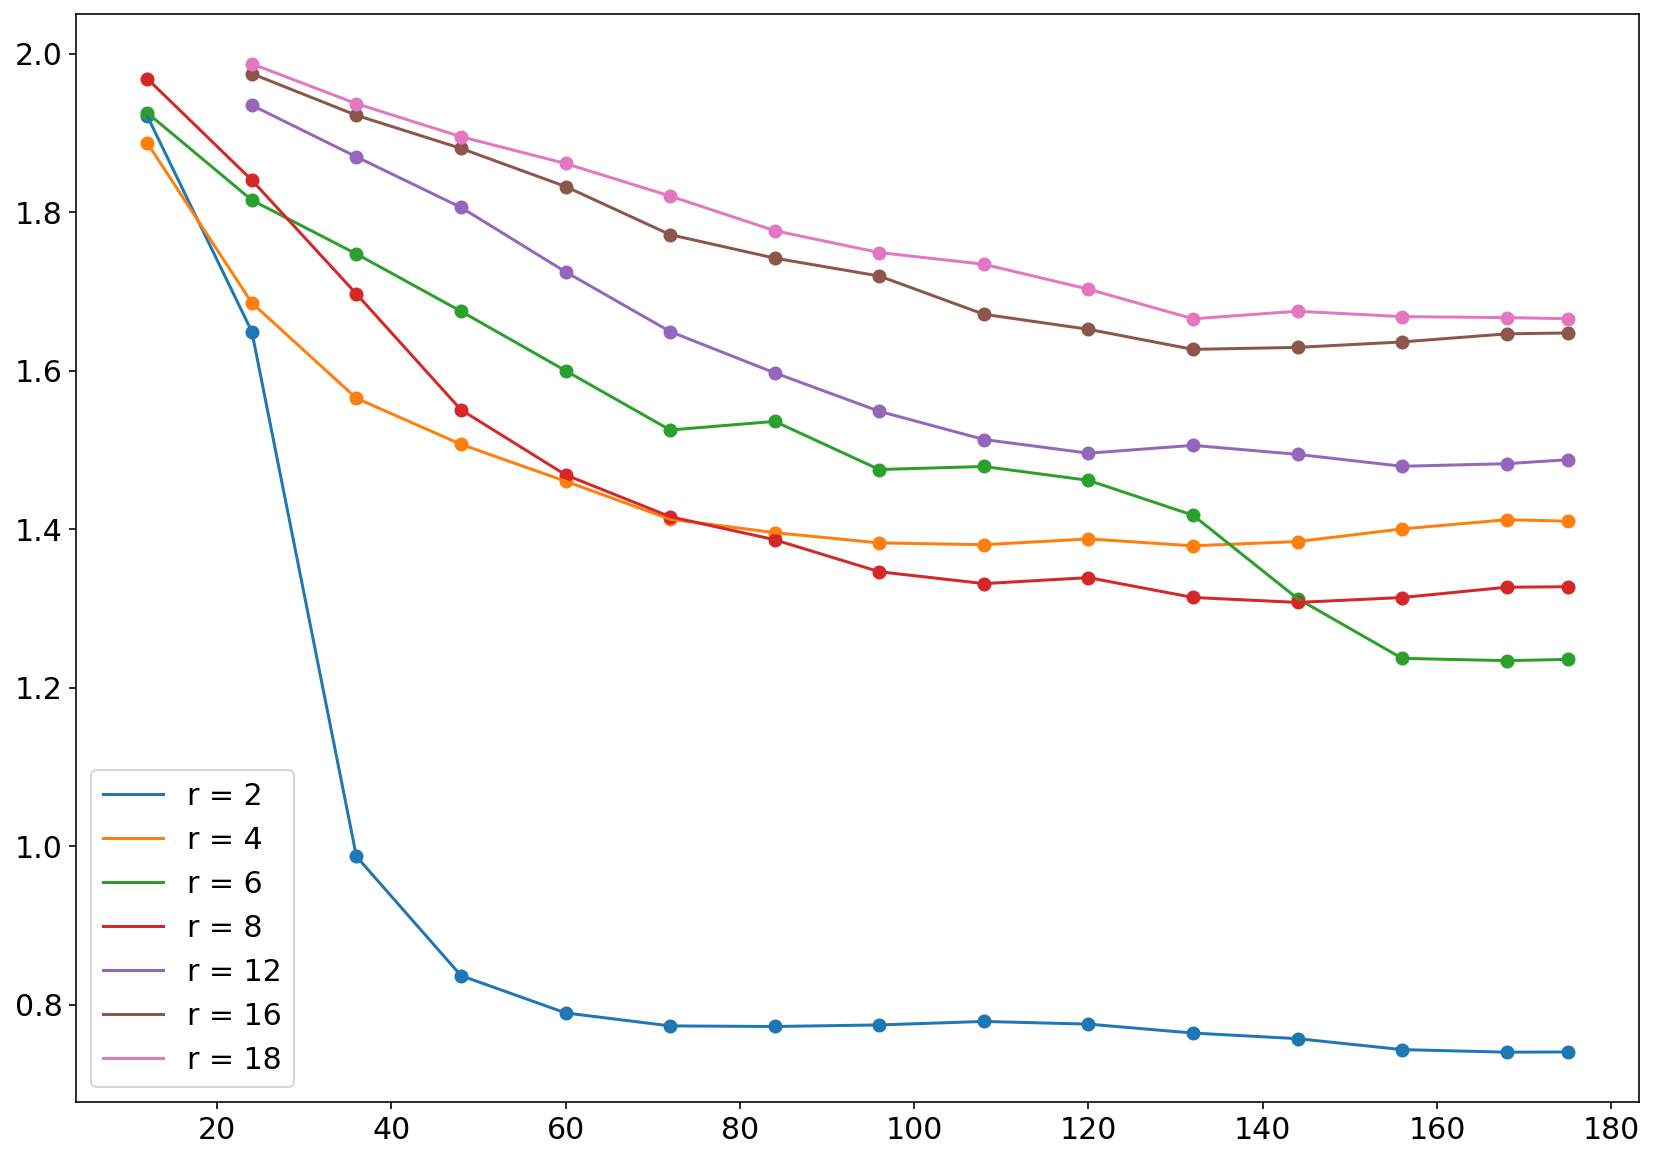
\includegraphics[width=0.9\linewidth]{imgs/comp/ser/ssa_reconstruct}}
	\caption{<<Сумма синусов с красным шумом>>. Ряд $\mathsf{V}_{650}$. Ошибка восстановление тренировочной части в зависимости от параметра $L$.}
	\label{serr_ssa_reconstruct}
\end{figure}

Ниже на графиках представлены результаты. Видно, что лучше всего метод SSA восстанавливает сигнал с параметрами $L = 175, \; r = 2$ (рис. \ref{ser_ssa_LH_r2}). Для остальных пар наблюдается влияние шума. На рисунках \multiref{ser_ssa_LH_r6}{ser_ssa_L84_r14} можно наблюдать, что для параметров $L = 175$ и $r = \{4, 6\}$ влияние шума меньше, чем для пар $L = 36, \; r = 16$, $L = 84, \; r = 14$. На рисунке \ref{ser_ssa_r4_r6} можно заметить, что разницы в восстановленных сигналах для пар $L = 175 \; r = 4$ и $L = 175 \; r = 6$ не очень большая. Аналогичные выводы можно сделать для пар $L = 36, \; r = 16$, $L = 84, \; r = 14$ на рисунке \ref{ser_ssa_r14_r16}.

Далее в эксперименте рассмотрим три пары $L = 175, \; r = 2$, $L = 175, \; r = 4$ и $L = 84, \; r = 14$. Пара $L = 175, \; r = 2$ дает наилучшее восстановление ряда. Выбирая из пар $L = 36, \; r = 16$, $L = 84, \; r = 14$, взяли вторую, так как в теории она дает меньшую аппроксимацию оценкой сигнала ряда. Пару $L = 175, \; r = 4$ выбрали как аналитически верную.

\begin{figure}[H]
	\captionsetup{justification=centering}
	\center{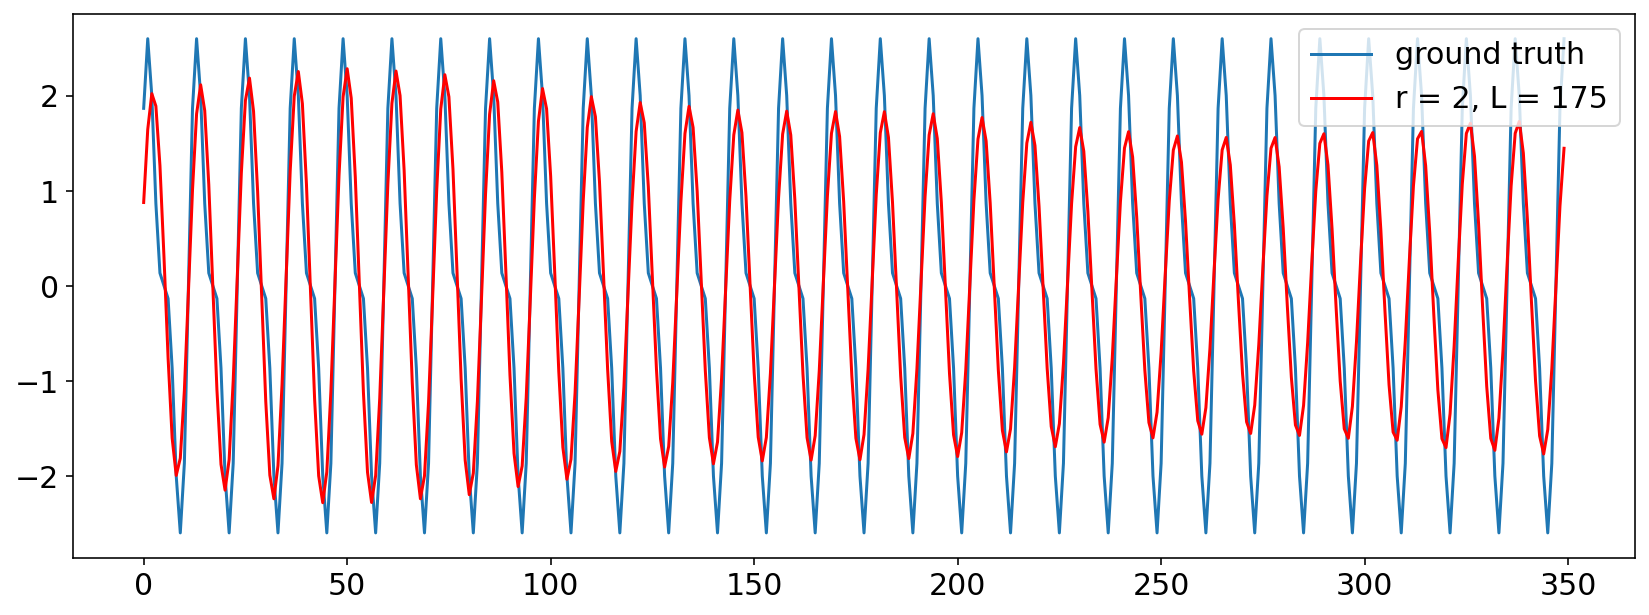
\includegraphics[width=0.9\linewidth]{imgs/comp/ser/ssa_LH_r2}}
	\caption{<<Сумма синусов с красным шумом>>. Ряд $\mathsf{V}_{650}$. Восстановление тренировочной выборки с помощью метода SSA. $L = 175, \; r = 2$.}
	\label{ser_ssa_LH_r2}
\end{figure}

\begin{figure}[H]
	\captionsetup{justification=centering}
	\center{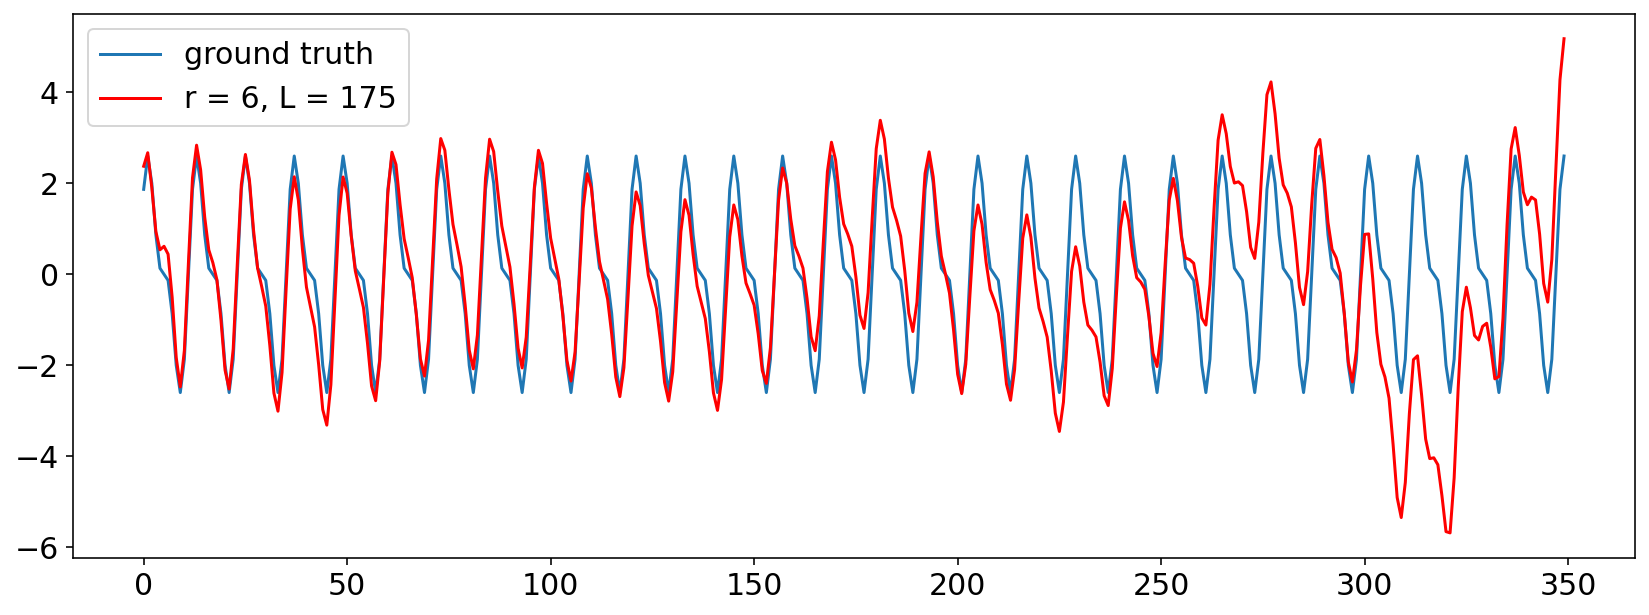
\includegraphics[width=0.9\linewidth]{imgs/comp/ser/ssa_LH_r6}}
	\caption{<<Сумма синусов с красным шумом>>. Ряд $\mathsf{V}_{650}$. Восстановление тренировочной выборки с помощью метода SSA. $L = 175, \; r = 6$.}
	\label{ser_ssa_LH_r6}
\end{figure}

\begin{figure}[H]
	\captionsetup{justification=centering}
	\center{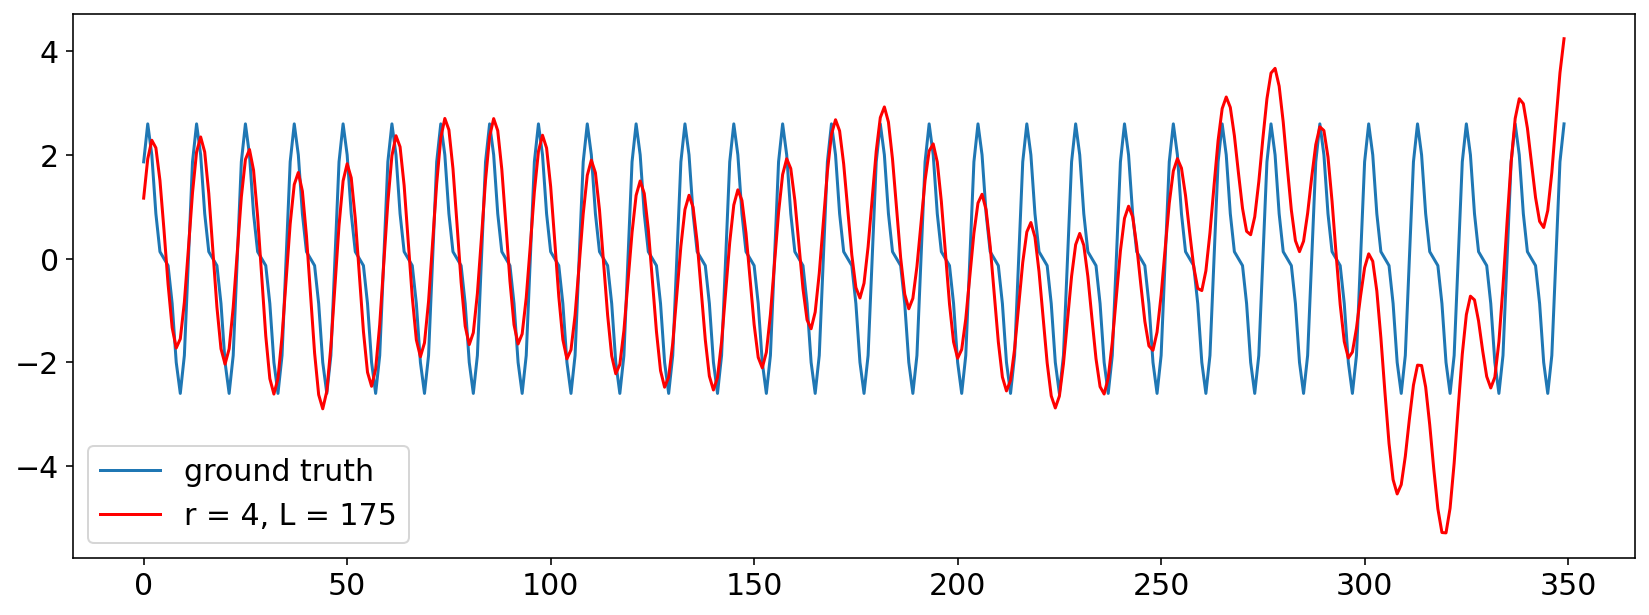
\includegraphics[width=0.9\linewidth]{imgs/comp/ser/ssa_LH_r4}}
	\caption{<<Сумма синусов с красным шумом>>. Ряд $\mathsf{V}_{650}$. Восстановление тренировочной выборки с помощью метода SSA. $L = 175, \; r = 4$.}
	\label{ser_ssa_LH_r4}
\end{figure}

\begin{figure}[H]
	\captionsetup{justification=centering}
	\center{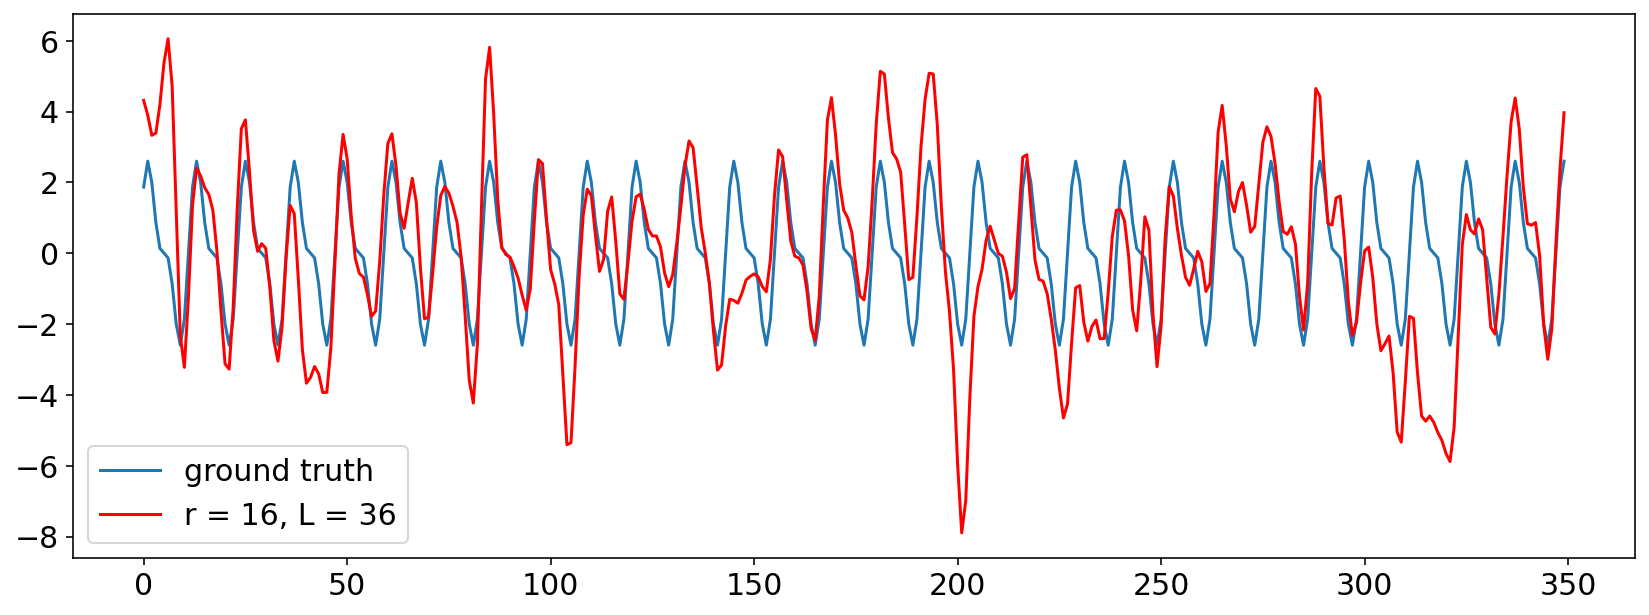
\includegraphics[width=0.9\linewidth]{imgs/comp/ser/ssa_L36_r16}}
	\caption{<<Сумма синусов с красным шумом>>. Ряд $\mathsf{V}_{650}$. Восстановление тренировочной выборки с помощью метода SSA. $L = 36, \; r = 16$.}
	\label{ser_ssa_L36_r16}
\end{figure}

\begin{figure}[H]
	\captionsetup{justification=centering}
	\center{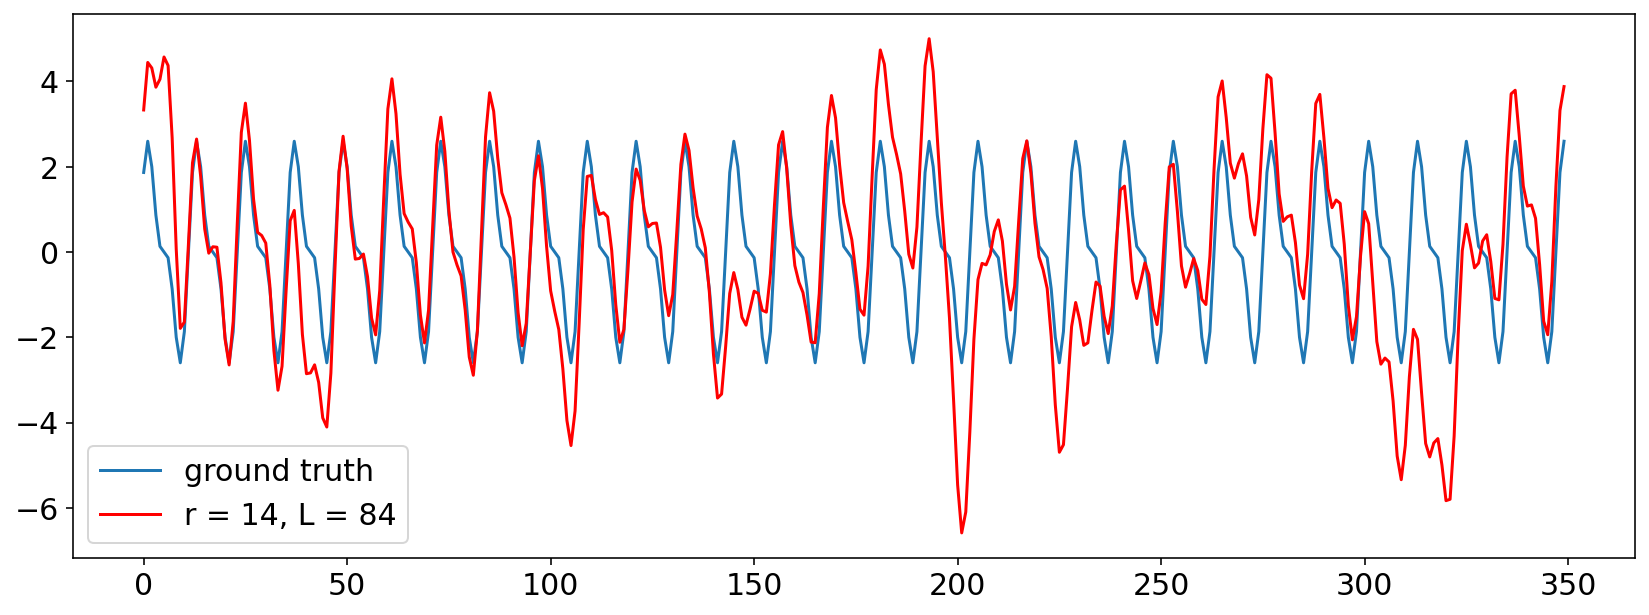
\includegraphics[width=0.9\linewidth]{imgs/comp/ser/ssa_L84_r14}}
	\caption{<<Сумма синусов с красным шумом>>. Ряд $\mathsf{V}_{650}$. Восстановление тренировочной выборки с помощью метода SSA. $L = 84, \; r = 14$.}
	\label{ser_ssa_L84_r14}
\end{figure}

\begin{figure}[H]
	\captionsetup{justification=centering}
	\center{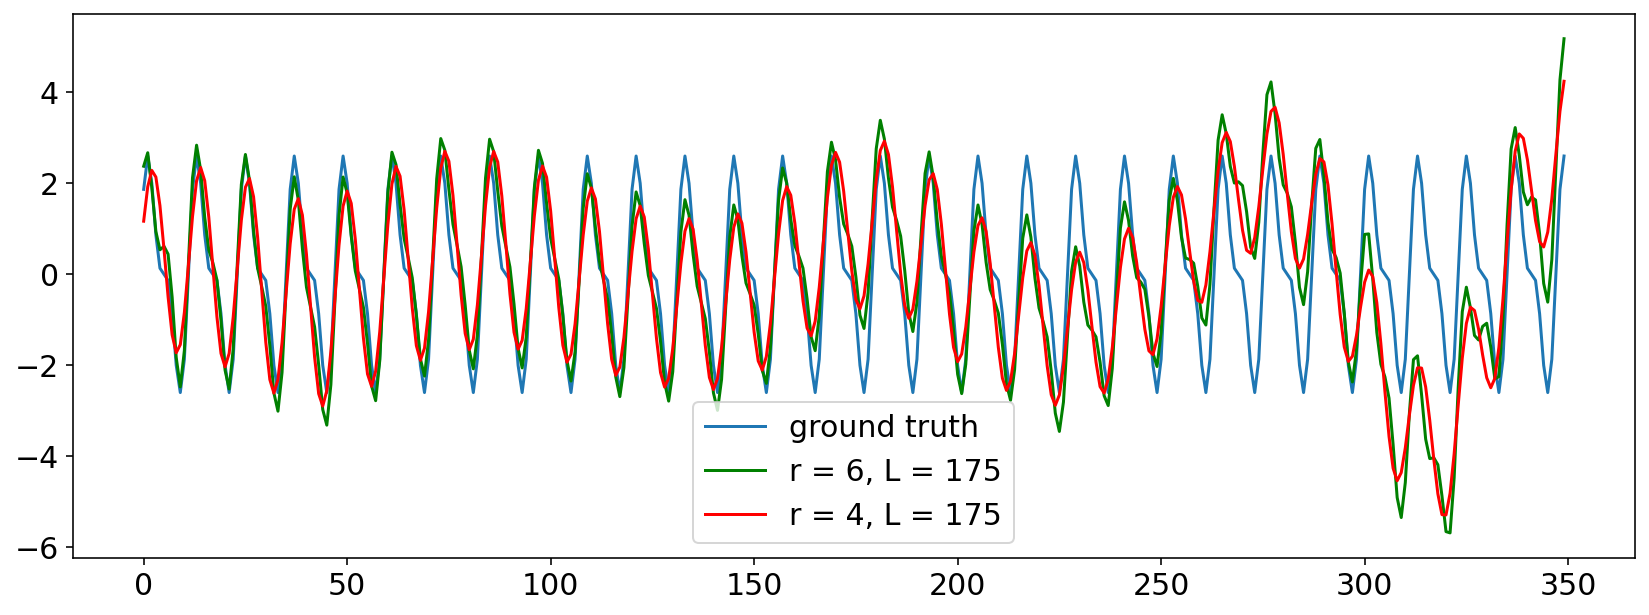
\includegraphics[width=0.9\linewidth]{imgs/comp/ser/ssa_r4_r6}}
	\caption{<<Сумма синусов с красным шумом>>. Ряд $\mathsf{V}_{650}$. Восстановление тренировочной выборки с помощью метода SSA. $L = 175, \; r = 4$ и $L = 175, \; r = 6$.}
	\label{ser_ssa_r4_r6}
\end{figure}

\begin{figure}[H]
	\captionsetup{justification=centering}
	\center{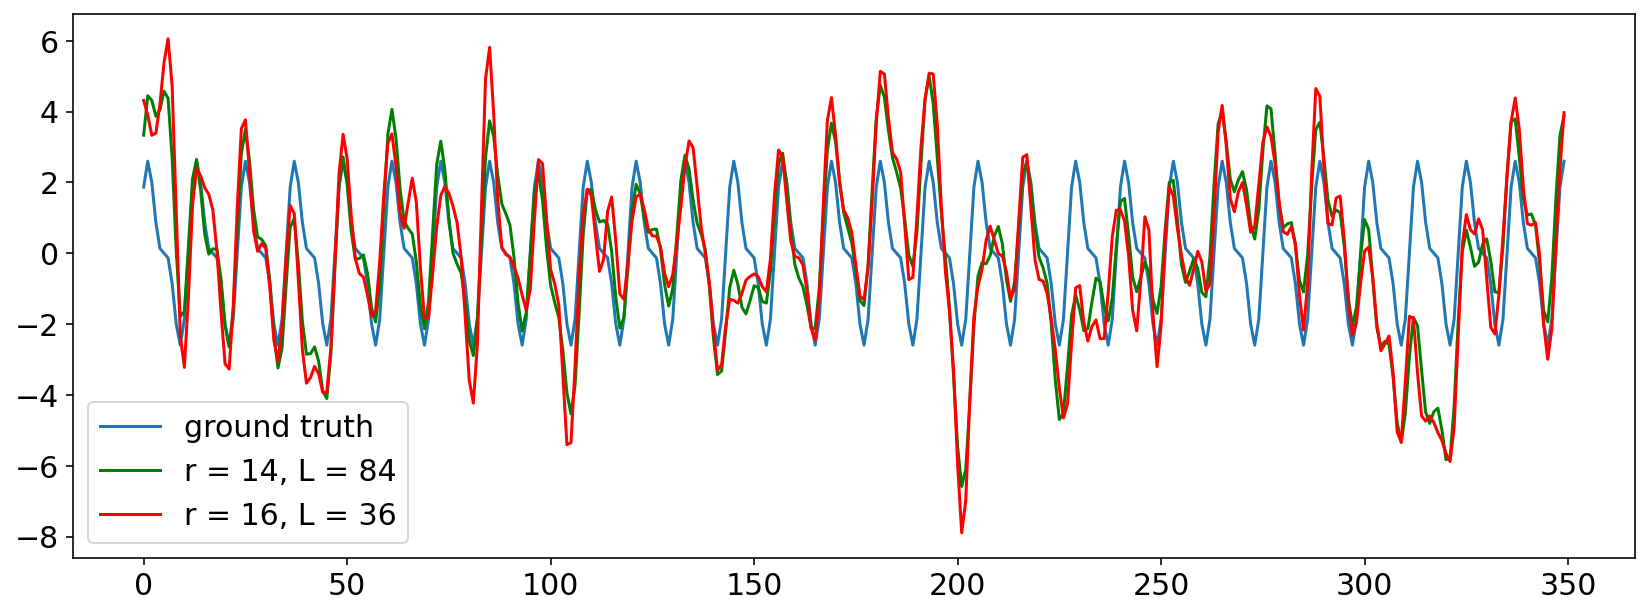
\includegraphics[width=0.9\linewidth]{imgs/comp/ser/ssa_r16_r14}}
	\caption{<<Сумма синусов с красным шумом>>. Ряд $\mathsf{V}_{650}$. Восстановление тренировочной выборки с помощью метода SSA. $L = 84, \; r = 14$ и $L = 36, \; r = 16$.}
	\label{ser_ssa_r14_r16}
\end{figure}

\subsubsection{Сравнение обычных и гибридных методов}
\label{serr_comp}

Для нейронных сетей зададим следующую сетку параметров: $T = \{12, 24, \ldots, 132 \}$, $h = \{10, 25, \ldots, 100 \}$. Для метода SSA в гибридных моделях возьмем пары параметров, выбранные выше.

Для прогноза по методу SSA зададим сетку, что была ранее: $L = \{ 12, 24, \ldots, 175 \}$, $r = \{ 2, 4, 6, 8, 10, 12, 16 \}$.

Будем сравнивать получившиеся прогнозы относительно сигнала и временного ряда. На графиках \multiref{serr_r2}{serr_r14} (больше графиков в приложении \ref{aserr_comp}) представлены результаты сравнения относительно временного ряда, диапазон ошибки на оси ординат лежит от $1.3$ до $2.2$. На графиках \multiref{sigserr_r2}{sigserr_r14} результаты сравнения относительно сигнала ряда, диапазон ошибки на оси ординат лежит от $0.25$ до $2.2$.

На графиках, где показано отклонение от временного ряда, можно заметить, что гибридные методы сильно проигрывают обычным методам. На графике \ref{serr_r2} можно видеть среднюю ошибку $2.09$ для гибридных моделей с параметрами $L = 175, \; r = 2$. На графике \ref{serr_r4} средняя ошибка достигает $2.07$ для гибридных моделей с параметрами $L = 175, \; r = 4$. На графике \ref{serr_r14} средняя ошибка падает до $1.95$ для гибридных моделей с параметрами $L = 84, \; r = 14$. Для обычных методов средняя ошибка составляет примерно $1.4$.

На графиках, где показано отклонение от сигнала ряда, можно наблюдать совершенно противоположную ситуацию. Ошибка прогноза гибридных методов сильно упала, а вот ошибка прогноза обычных методов выросла до $1.6$. На графике \ref{sigserr_r2} можно видеть среднюю ошибку $0.37$ для гибридных моделей с параметрами $L = 175, \; r = 2$. На графике \ref{sigserr_r4} средняя ошибка достигает $0.87$ для гибридных моделей с параметрами $L = 175, \; r = 4$. На графике \ref{sigserr_r14} средняя ошибка $1.49$ для гибридных моделей с параметрами $L = 84, \; r = 14$.

Можно заметить, что средняя ошибка для обычных нейронных сетей составляет, как уже говорилось, $1.4$, если считать отклонение от ряда. В случае, если считать отклонение от сигнала, средняя ошибка увеличивается до значение $1.6$. Эффект легко заметить на графиках ниже. Можно сделать вывод, что обычные нейронные сети пытаются прогнозировать ряд вместе с шумом.

Также видна тенденция, что чем больше параметр $r$ в гибридных моделях, тем меньше ошибка, посчитанная относительно отклонения от временного ряда. А чем меньше параметр $r$, тем меньше ошибка, посчитанная относительно отклонения от сигнала ряда. Это говорит о том, что обычные и гибридные методы решают две разные задачи в случае красного шума. Обычные методы пытаются прогнозировать временной ряд вместе шумом. Гибридные методы прогнозируют сигнал ряда, при условии что в оценку ряда не попал существенное количество шумовых компонент.

\begin{figure}[H]
	\captionsetup{justification=centering}
	\center{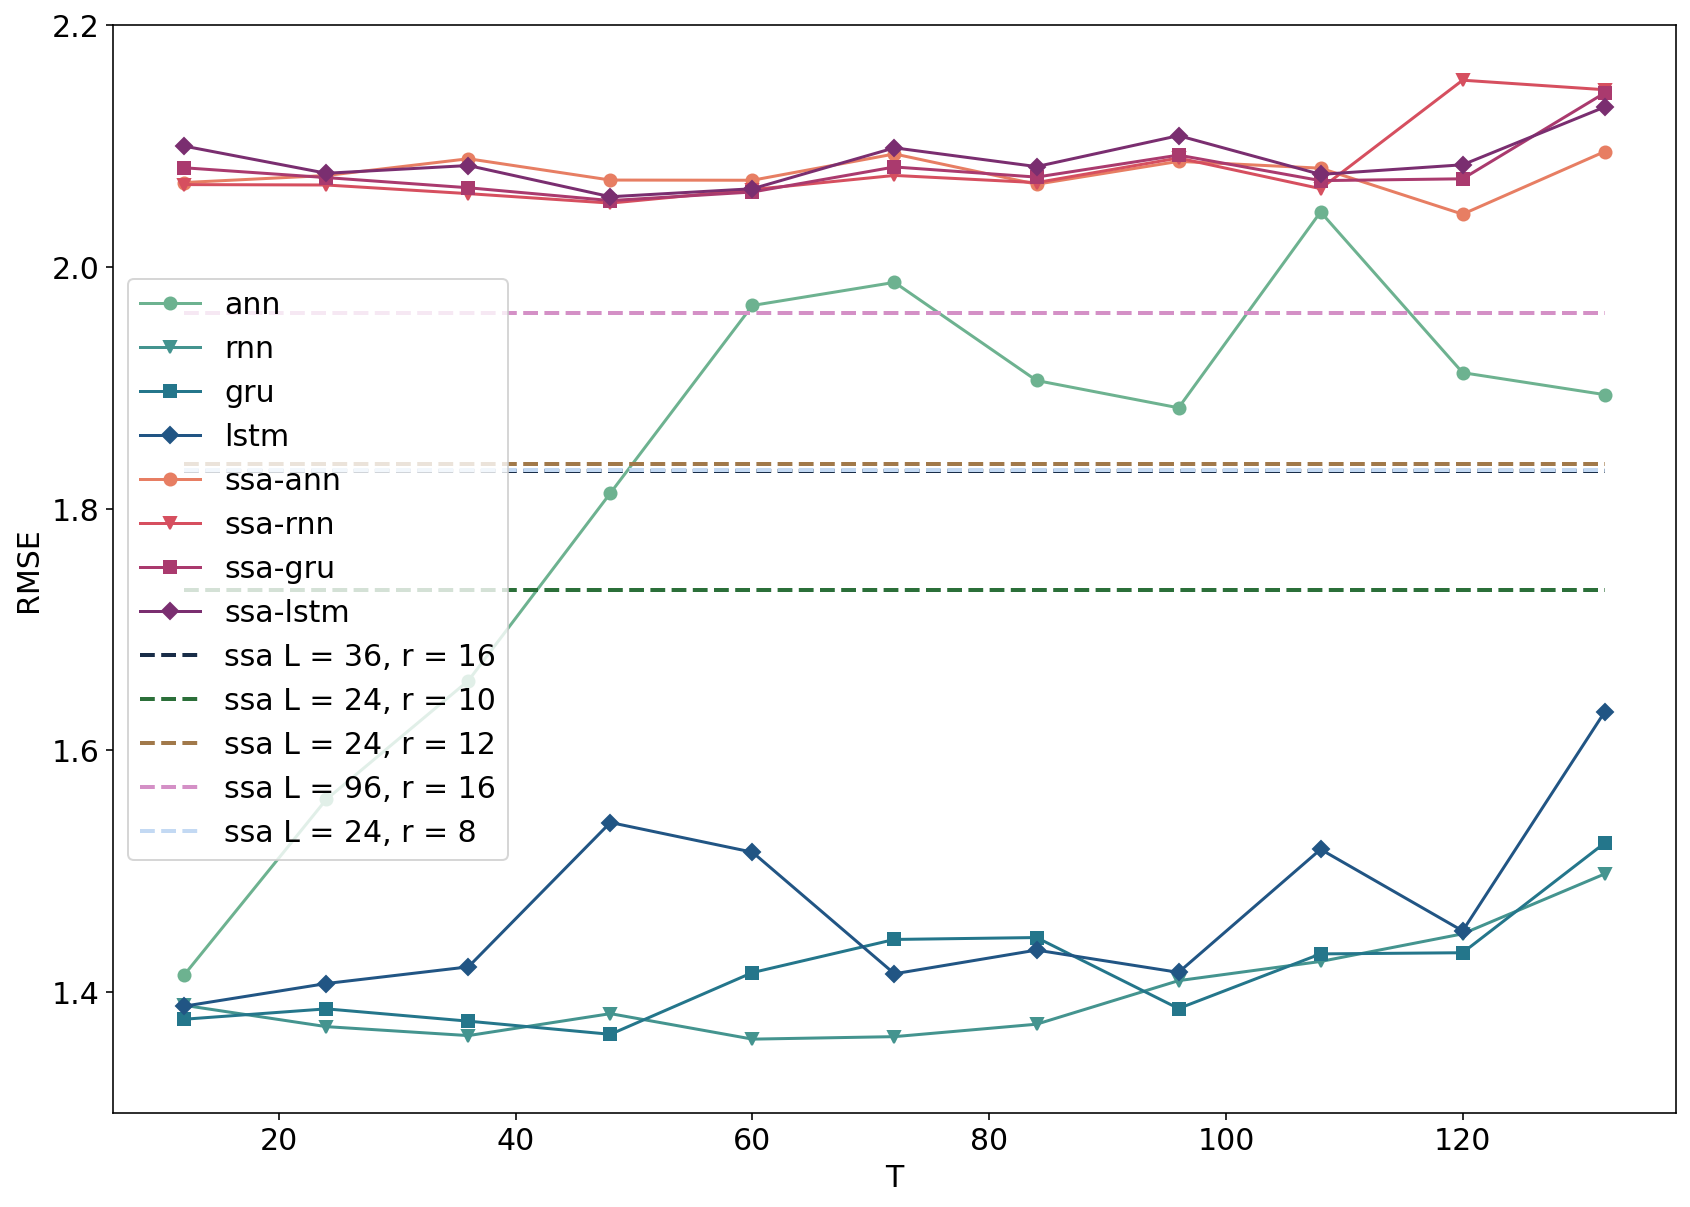
\includegraphics[width=0.9\linewidth, height=0.6\linewidth]{imgs/comp/ser/serr_r2}}
	\caption{<<Сумма синусов с красным шумом>>. Ряд $\mathsf{V}_{650}$. Ошибки прогноза относительно ряда в зависимости от параметра $T$. $L = 175, \; r = 2$.}
	\label{serr_r2}
\end{figure}

\begin{figure}[H]
	\captionsetup{justification=centering}
	\center{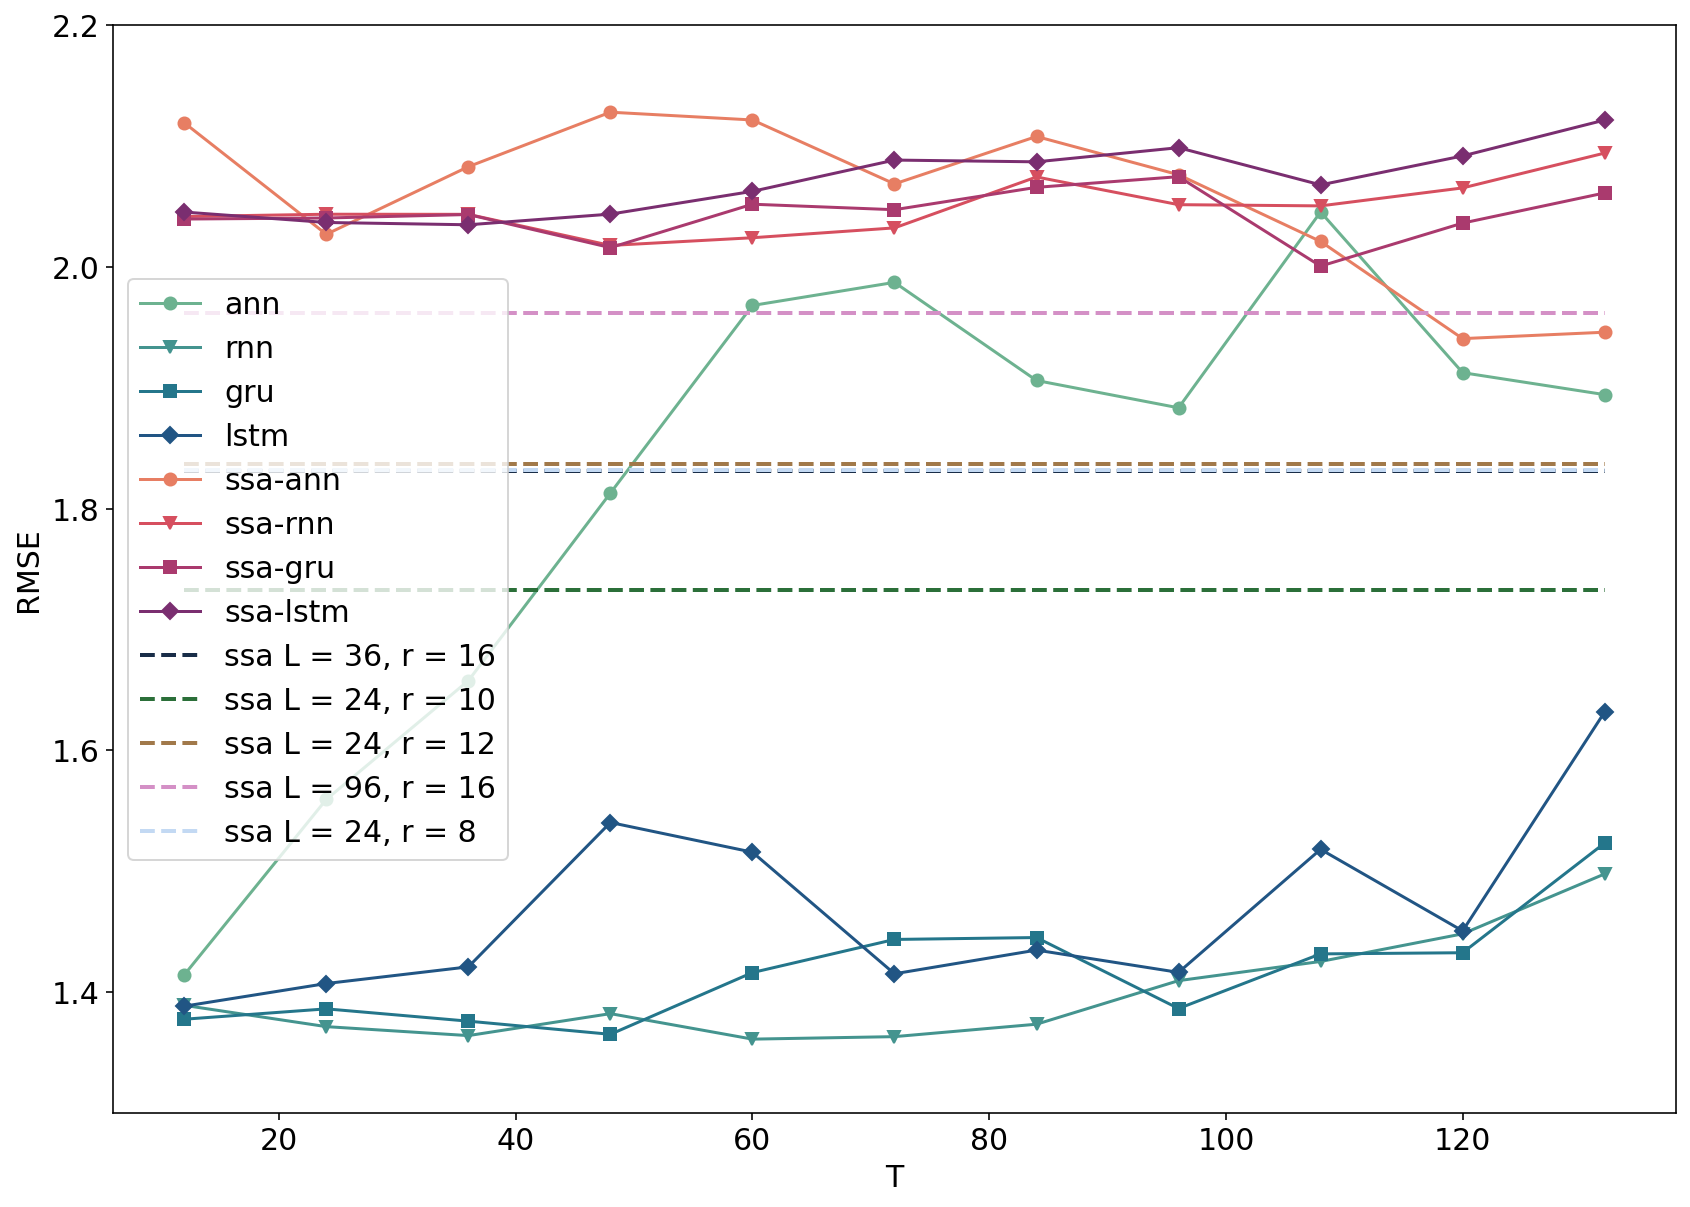
\includegraphics[width=0.9\linewidth, height=0.6\linewidth]{imgs/comp/ser/serr_r4}}
	\caption{<<Сумма синусов с красным шумом>>. Ряд $\mathsf{V}_{650}$. Ошибки прогноза относительно ряда в зависимости от параметра $T$. $L = 175, \; r = 4$.}
	\label{serr_r4}
\end{figure}

\begin{figure}[H]
	\captionsetup{justification=centering}
	\center{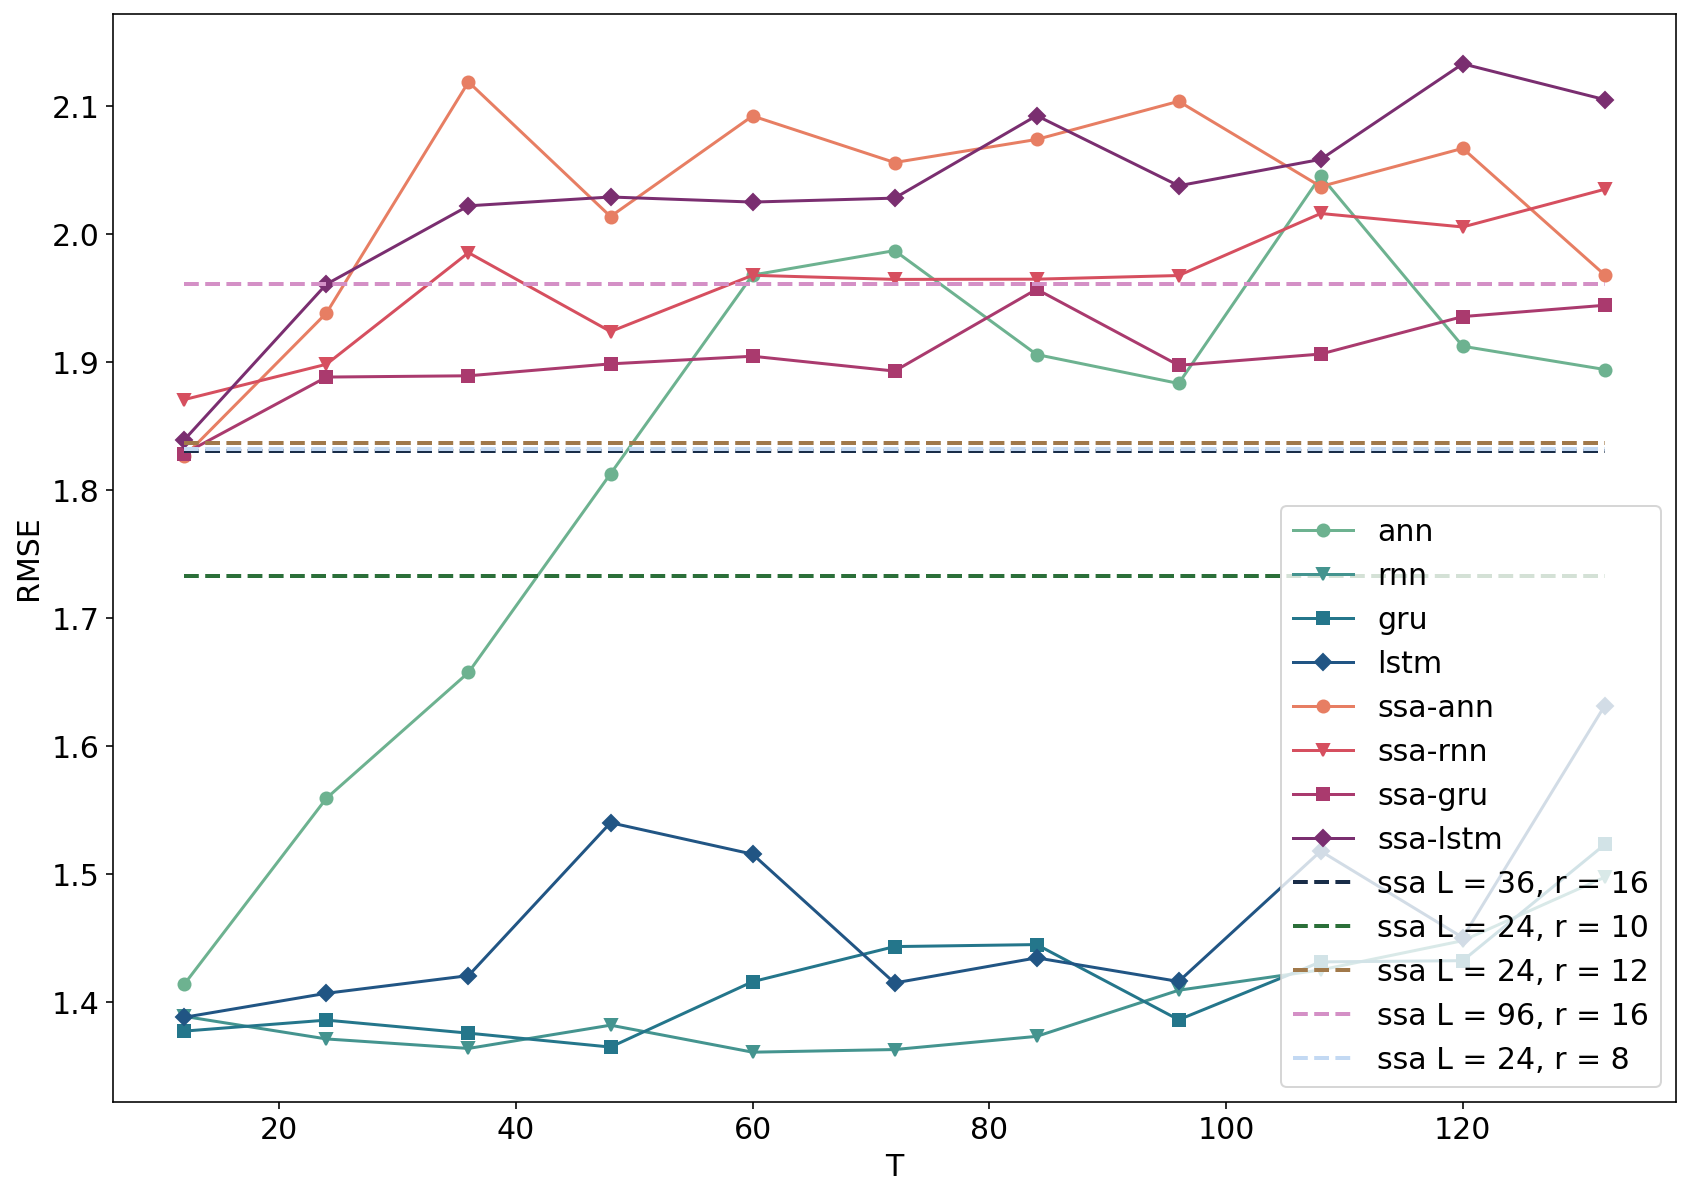
\includegraphics[width=0.9\linewidth, height=0.6\linewidth]{imgs/comp/ser/serr_r14}}
	\caption{<<Сумма синусов с красным шумом>>. Ряд $\mathsf{V}_{650}$. Ошибки прогноза относительно ряда в зависимости от параметра $T$. $L = 84, \; r = 14$.}
	\label{serr_r14}
\end{figure}

\begin{figure}[H]
	\captionsetup{justification=centering}
	\center{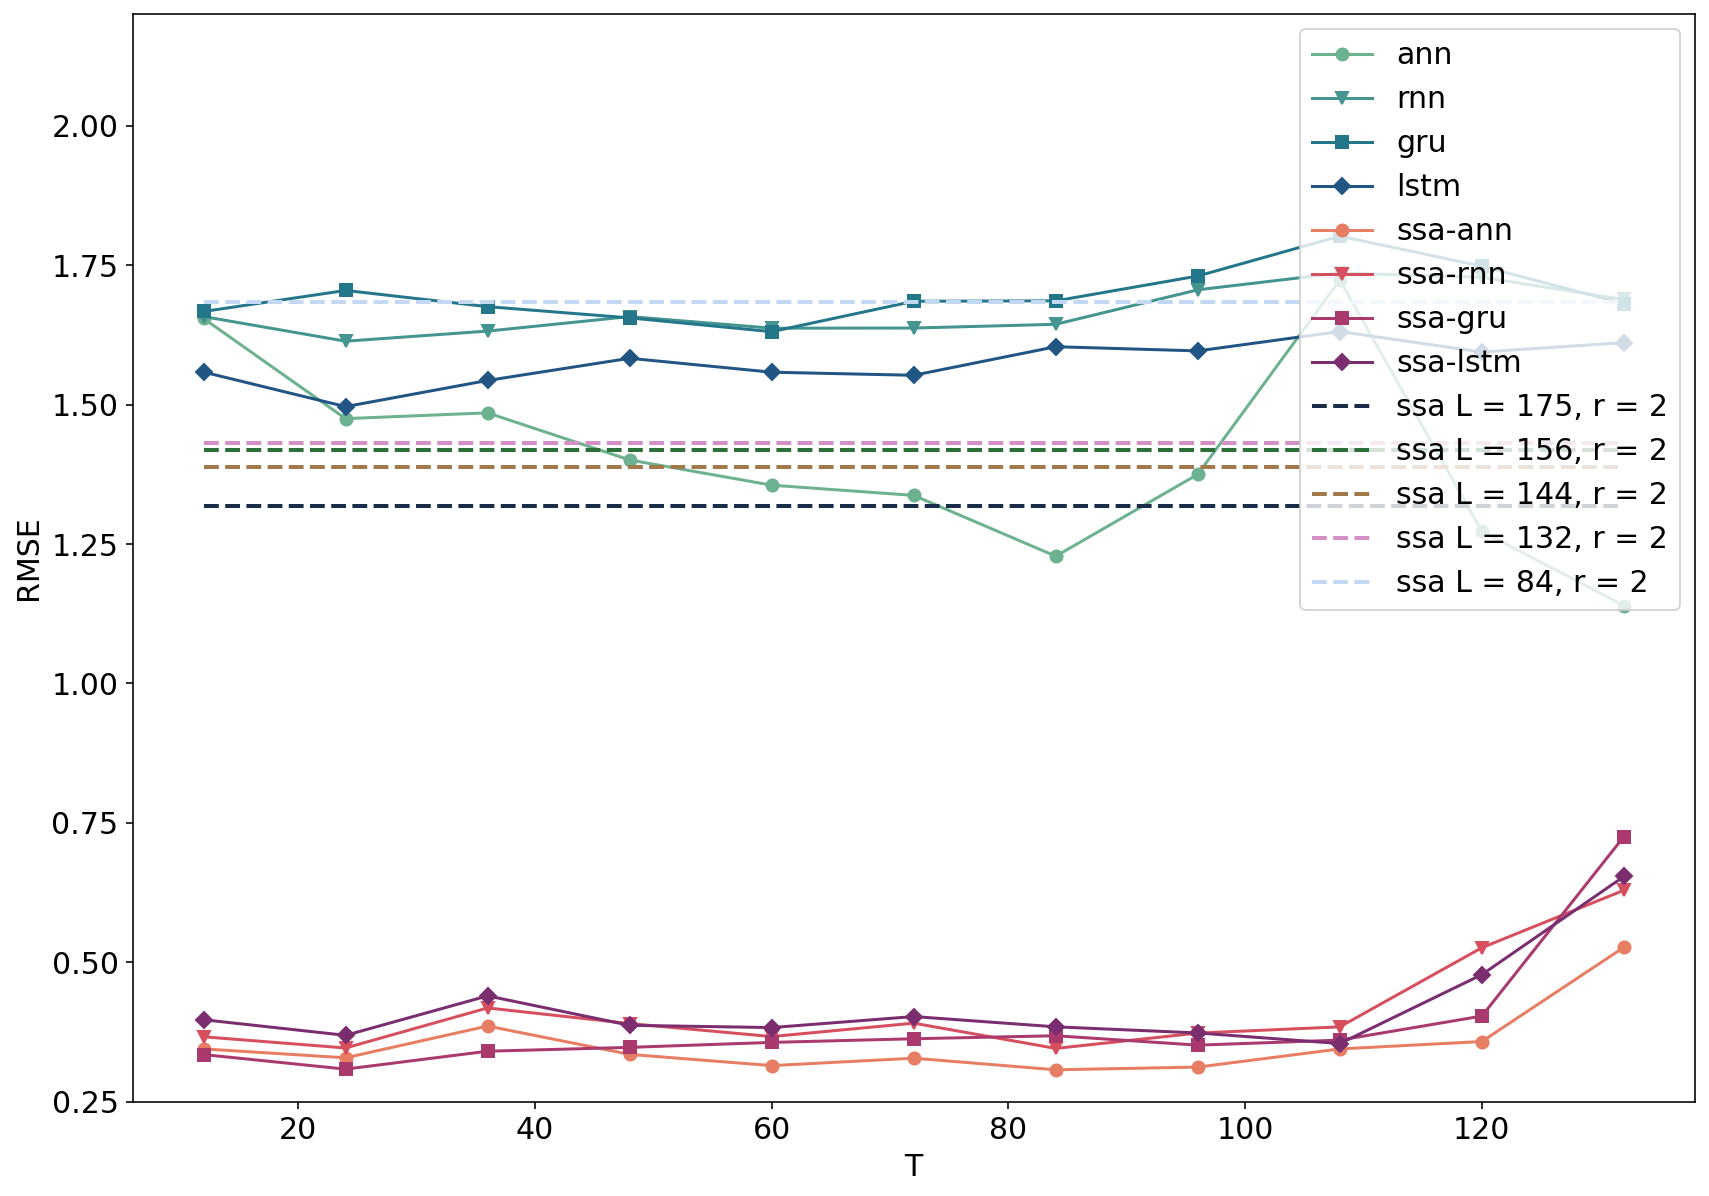
\includegraphics[width=0.9\linewidth, height=0.6\linewidth]{imgs/comp/ser/sigserr_r2}}
	\caption{<<Сумма синусов с красным шумом>>. Ряд $\mathsf{V}_{650}$. Ошибки прогноза относительно сигнала в зависимости от параметра $T$. $L = 175, \; r = 2$.}
	\label{sigserr_r2}
\end{figure}

\begin{figure}[H]
	\captionsetup{justification=centering}
	\center{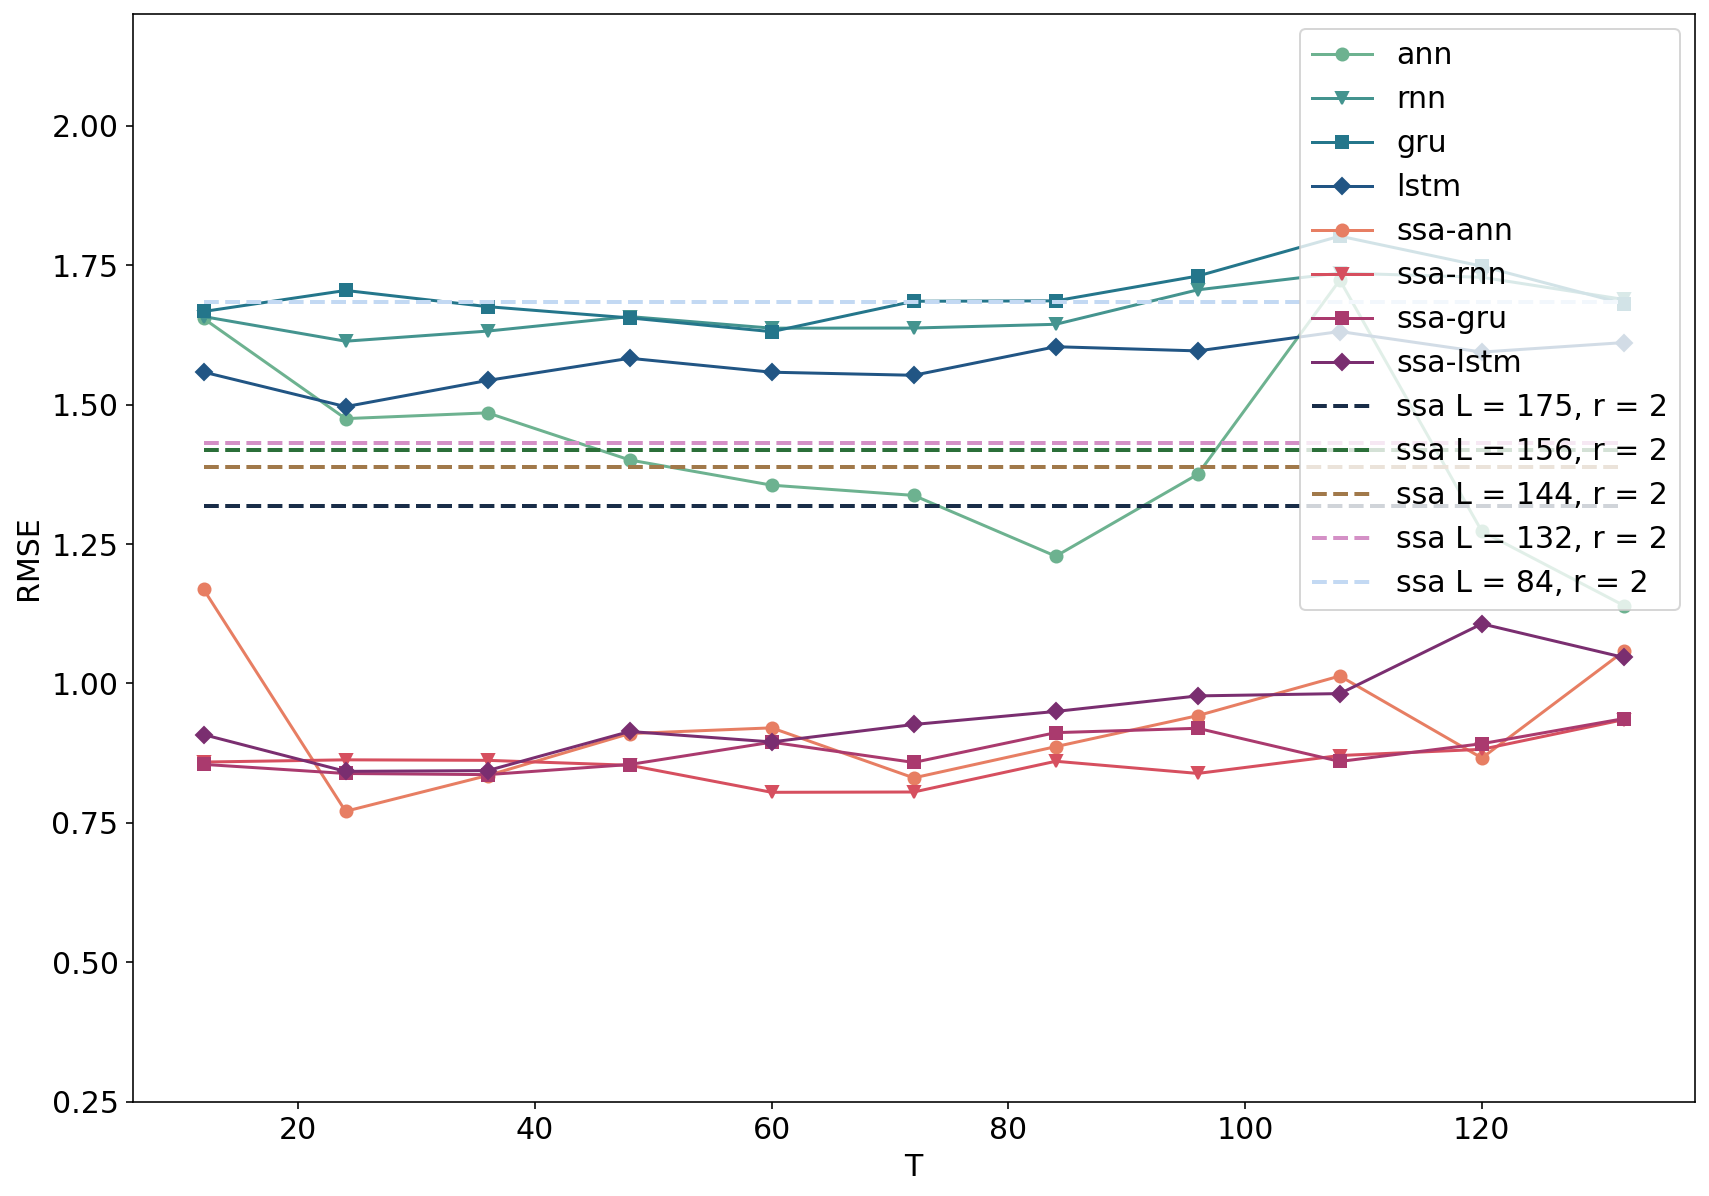
\includegraphics[width=0.9\linewidth, height=0.6\linewidth]{imgs/comp/ser/sigserr_r4}}
	\caption{<<Сумма синусов с красным шумом>>. Ряд $\mathsf{V}_{650}$. Ошибки прогноза относительно сигнала в зависимости от параметра $T$. $L = 175, \; r = 4$.}
	\label{sigserr_r4}
\end{figure}

\begin{figure}[H]
	\captionsetup{justification=centering}
	\center{\includegraphics[width=0.9\linewidth, height=0.6\linewidth]{imgs/comp/ser/sigserr_r14}}
	\caption{<<Сумма синусов с красным шумом>>. Ряд $\mathsf{V}_{650}$. Ошибки прогноза относительно сигнала в зависимости от параметра $T$. $L = 84, \; r = 14$.}
	\label{sigserr_r14}
\end{figure}

\subsubsection{Отображение прогнозов}
\label{serr_res}

На графиках \multiref{serr_r2_res_ann}{serr_r14_res_rnn} (больше графиков в приложении \ref{aserr_res}) представлены результаты прогнозирования методами (на графиках показано отклонение от сигнала ряда). Можем заметить, как сильно обычные методы пытаются предсказывать шум. Для пары $L = 84, \; r = 14$ у гибридных методов предсказание сигнала получилось не очень хорошее. Это объяснимо тем, что в оценке сигнала попало слишком много шумовых компонент. Для пары $L = 175, \; r = 4$ получилось хорошее предсказание сигнала методов SSA-RNN и SSA-GRU. Для пары $L = 175, \; r = 2$ хорошее предсказание получилось для трех методов SSA-RNN, SSA-GRU и SSA-LSTM.

\begin{figure}[H]
	\captionsetup{justification=centering}
	\center{\includegraphics[width=0.9\linewidth]{imgs/comp/ser/serr_r2_res_ann}}
	\caption{<<Сумма синусов с красным шумом>>. Ряд $\mathsf{V}_{650}$. Прогноз результатов для ANN и SSA-ANN. $L = 175, \; r = 2$}
	\label{serr_r2_res_ann}
\end{figure}

\begin{figure}[H]
	\captionsetup{justification=centering}
	\center{\includegraphics[width=0.9\linewidth]{imgs/comp/ser/serr_r2_res_rnn}}
	\caption{<<Сумма синусов с красным шумом>>. Ряд $\mathsf{V}_{650}$. Прогноз результатов для RNN и SSA-RNN. $L = 175, \; r = 2$}
	\label{serr_r2_res_rnn}
\end{figure}

\begin{figure}[H]
	\captionsetup{justification=centering}
	\center{\includegraphics[width=0.9\linewidth]{imgs/comp/ser/serr_r4_res_ann}}
	\caption{<<Сумма синусов с красным шумом>>. Ряд $\mathsf{V}_{650}$. Прогноз результатов для ANN и SSA-ANN. $L = 175, \; r = 4$}
	\label{serr_r4_res_ann}
\end{figure}

\begin{figure}[H]
	\captionsetup{justification=centering}
	\center{\includegraphics[width=0.9\linewidth]{imgs/comp/ser/serr_r4_res_rnn}}
	\caption{<<Сумма синусов с красным шумом>>. Ряд $\mathsf{V}_{650}$. Прогноз результатов для RNN и SSA-RNN. $L = 175, \; r = 4$}
	\label{serr_r4_res_rnn}
\end{figure}

\begin{figure}[H]
	\captionsetup{justification=centering}
	\center{\includegraphics[width=0.9\linewidth]{imgs/comp/ser/serr_r14_res_ann}}
	\caption{<<Сумма синусов с красным шумом>>. Ряд $\mathsf{V}_{650}$. Прогноз результатов для ANN и SSA-ANN. $L = 84, \; r = 14$}
	\label{serr_r14_res_ann}
\end{figure}

\begin{figure}[H]
	\captionsetup{justification=centering}
	\center{\includegraphics[width=0.9\linewidth]{imgs/comp/ser/serr_r14_res_rnn}}
	\caption{<<Сумма синусов с красным шумом>>. Ряд $\mathsf{V}_{650}$. Прогноз результатов для RNN и SSA-RNN. $L = 84, \; r = 14$}
	\label{serr_r14_res_rnn}
\end{figure}

\subsubsection{Проверка устойчивости}
\label{serr_rob}

Чтобы исключить случайность в полученных результатах, проведем сравнение для разных начальных весов методов. Зафиксируем новую сетку для параметра $T = \{12, 84\}$. Сетка для параметра $h$ останется прежней. Будем получать каждый результат по 7 раз, инициализируя метод с новыми весами. Полученные результаты отображены на рисунках \multiref{serrloopsr2.12}{sigserrloopsr14.84} в приложении \ref{aserr_rob}. На них подтверждается, выводы сделанные ранее. Заключаем, что полученные результаты устойчивые.

\subsubsection{Выводы}

Из полученных результатов и таблицы \ref{tserr} (таблица является аналогичной таблице \ref{tedsiner}) видно, что при красном шуме обычные нейронные сети прогнозируют временной ряд вместе с шумом и выполняют эту задачу лучше, чем гибридные методы, что логично, так как в гибридных методах на вход сети подается сигнал без шума. Метод SSA находится между ними при ошибке относительно всего ряда.

Если считать ошибку относительно сигнала ряда, гибридные методы показывают наименьшие значения ошибки. Метод SSA в этом случае прогнозируют сигнал ряда точнее, чем негибридные. Заметно, что чем больше $r$, тем существенно больше ошибка у гибридных методов. Это объяснимо тем, что в оценку сигнала попадает шум.

Эксперимент также показал, что при прогнозе сигнала желательно выбирать параметр $r$ ниже оптимального, если есть вероятность смешивания шума с сигналом ряда. Так даже, если сигнал не был полностью восстановлен, то нейронная в гибридном методе сеть сможет корректно спрогнозировать сигнал ряда. Это было продемонстрировано для пары параметров SSA $r = 2, \; L = 175$, гибридные методы получили среднюю ошибку $0.37$, в сравнении с $1.6$ для обычных методов.

Таблица~\ref{bigtable} показывает, что из негибридных метод RNN достигают наилучших результатов, если считать отклонение от всего ряда. Среди гибридных методов лучше всего работает SSA-GRU. Если смотреть отклонение от сигнала ряда, то лучшие результаты показывает гибридный метод SSA-ANN. Из негибридных метод хорошо работает ANN.

\begin{table}[h]
	\captionsetup{justification=centering}
	\caption{<<Сумма синусов с красным шумом>>. Ряд $\mathsf{V}_{650}$. Усредненные и лучшие результаты прогнозов по RMSE относительно всего ряда и сигнала.}
	\begin{center}
		\begin{tabular}{ccccc}
			\toprule
			{ssa-params} &  b-nn &  m-nn &  b-ssa &  m-ssa \\
			\midrule
			-          & 1.294 & 1.523 &  1.733 &  1.803 \\
			$L = 175, \; r = 2$       & 1.939 & 2.083 &  1.733 &  1.803 \\
			$L = 175, \; r = 4$       & 1.850 & 2.056 &  1.733 &  1.803 \\
			$L = 84, \; r = 14$     & 1.736 & 1.989 &  1.733 &  1.803 \\
			\midrule
			-          & 0.999 & 1.589 &  1.319 &  1.398 \\
			$L = 175, \; r = 2$       & 0.164 & 0.385 &  1.319 &  1.398 \\
			$L = 175, \; r = 4$       & 0.694 & 0.898 &  1.319 &  1.398 \\
			$L = 84, \; r = 14$     & 0.998 & 1.489 &  1.319 &  1.398 \\
			\bottomrule
		\end{tabular}
	\end{center}
	\label{tserr}
\end{table}

\section{Суммарные результаты по модельный рядам}
В таблице~\ref{bigtable} собраны результаты по всем модельным примерам. Жирным шрифтом выделены лучшие результаты по средним ошибкам среди негибридных или гибридных методов для каждого модельного ряда.

Можно заметить, что чаще всего лучшие результаты достигались методами ANN и GRU и их гибридными аналогами SSA-ANN, SSA-GRU. Напротив, методы LSTM и SSA-LSTM не показали лучших результатов.

\begin{landscape}
\begin{table}[h]
	\caption{RMSE для модельных примеров.}
	\small
	\begin{center}
		\begin{tabular}{|cc||cc|cc|cc|cc||cc|}
			\toprule
			experiment & ssa-params        &  b-ann &  m-ann &  b-rnn &  m-rnn &  b-gru &  m-gru &  b-lstm &  m-lstm &  b-ssa &  m-ssa \\
			\midrule
			$\mathsf{Z}_{650}$ & - &  1.577 &  1.657 &  1.547 &  1.635 &  1.563 &  \textbf{1.623} &   1.566 &   1.625 &  1.581 &  1.586 \\
			& $L = 175, \; r = 2$ &  1.528 &  \textbf{1.558} &  1.554 &  1.571 &  1.545 &  1.566 &   1.545 &   1.574 &  1.581 &  1.586 \\
			& $L = 175, \; r = 4$ &  1.542 &  1.567 &  1.551 &  1.587 &  1.532 &  1.566 &   1.551 &   1.581 &  1.581 &  1.586 \\
			& $L = 175, \; r = 6$ &  1.533 &  1.578 &  1.557 &  1.614 &  1.563 &  1.629 &   1.592 &   1.632 &  1.581 &  1.586 \\
			$\mathsf{Z}_{1500}$ & - &  1.506 &  1.574 &  1.506 &  1.549 &  1.504 &  \textbf{1.538} &   1.511 &   1.539 &  1.511 &  1.512 \\
			& $L = 375, \; r = 4$ &  1.484 &  \textbf{1.513} &  1.494 &  1.520 &  1.495 &  1.519 &   1.496 &   1.529 &  1.511 &  1.512 \\
			$\mathsf{X}_{650}$ & - &  0.312 &  0.326 &  0.308 &  0.325 &  0.311 &  \textbf{0.321} &   0.314 &   0.330 &  0.315 &  0.316 \\
			& $L = 175, \; r = 2$ &  0.307 & \textbf{0.311}&  0.310 &  0.313 &  0.308 &  0.312 &   0.309 &   0.314 &  0.315 &  0.316 \\
			& $L = 175, \; r = 4$ &  0.306 &  0.312 &  0.309 &  0.316 &  0.305 &  0.312 &   0.307 &   0.317 &  0.315 &  0.316 \\
			& $L = 175, \; r = 6$ &  0.304 &  0.313 &  0.310 &  0.317 &  0.304 &  0.315 &   0.307 &   0.320 &  0.315 &  0.316 \\
			$\mathsf{V}_{650}$ & - &  1.381 &  1.819 &  1.316 &  \textbf{1.396} &  1.294 &  1.415 &   1.296 &   1.461 &  1.733 &  1.803 \\
			& $L = 175, \; r = 2$ &  1.939 &  2.078 &  2.014 &  2.088 &  2.025 &  2.078 &   2.021 &   2.088 &  1.733 &  1.803 \\
			& $L = 175, \; r = 4$ &  1.850 &  2.057 &  1.982 &  2.051 &  1.954 &  2.045 &   1.949 &   2.071 &  1.733 &  1.803 \\
			& $L = 84, \; r = 14$ &  1.781 &  2.031 &  1.801 &  1.968 &  1.736 &  \textbf{1.914} &   1.800 &   2.043 &  1.733 &  1.803 \\
			Сигнал $\mathsf{V}_{650}$ & - &  0.999 &  \textbf{1.404} &  1.451 &  1.679 &  1.527 &  1.697 &   1.340 &   1.577 &  1.319 &  1.398 \\
			& $L = 175, \; r = 2$ &  0.164 &  \textbf{0.349} &  0.287 &  0.404 &  0.275 &  0.367 &   0.286 &   0.421 &  1.319 &  1.398 \\
			& $L = 175, \; r = 4$ &  0.694 &  0.919 &  0.725 &  0.856 &  0.729 &  0.876 &   0.792 &   0.943 &  1.319 &  1.398 \\
			& $L = 84, \; r = 14$  &  0.998 &  1.443 &  1.238 &  1.475 &  1.221 &  1.439 &   1.339 &   1.597 &  1.319 &  1.398 \\
			\bottomrule
		\end{tabular}
	\end{center}
	\label{bigtable}
\end{table}
\end{landscape}

\chapter{Реальные данные}
\label{chapter_realdata}
\section{Среднемесячные осадки в Индии}
\label{indian_rain}

Рассмотри данные <<Indian Rain>>\footnote{Данные доступны для скачивания по ссылке \url{https://tropmet.res.in/static_pages.php?page_id=53} }, взятые из статьи \cite{ar1}. Рассмотрим первые $1500$ точек ряда, обозначим их как $\mathsf{Z}_{1500}$ (рис. \ref{indian_rain_img}). Данные <<Indian Rain>> показывают среднемесячное количество осадков в Индии.

\begin{figure}[H]
	\captionsetup{justification=centering}
	\center{\includegraphics[width=0.9\linewidth]{imgs/ts/indian_rain/indian_rain}}
	\caption{Данные <<Indian Rain>>. Ряд $\mathsf{Z}_{1500}$.}
	\label{indian_rain_img}
\end{figure}

В экспериментах будем разбивать ряд $\mathsf{Z}_{1500}$ на тренировочную, валидационную, тестовую выборки по $750, 500, 250$ точек соответственно.

На рисунке \ref{indian_rain_pgram} можно увидеть периодограмму ряда. Видно, что ряд имеет три периодики и трендовую составляющую. Исходя из рис. \ref{indian_rain_img} это константный тренд. Ввиду этого, будем считать параметры $r=7$ и $L = 375$ аналитически верными для метода SSA и гибридных методов, так как ранг ряда скорее всего равен $7$, а $L = 375$ удовлетворяет асимптотической разделимости. Также, так как это данные по месяцам, то период в ряде равен $12$. Далее в экспериментах будем перебирать параметры $T$ и $L$ по сетке с шагом кратным $12$.

\begin{figure}[H]
	\captionsetup{justification=centering}
	\center{\includegraphics[width=0.9\linewidth]{imgs/ts/indian_rain/indian_rain_pgram}}
	\caption{Данные <<Indian Rain>>. Периодограмма ряда $\mathsf{Z}_{1500}$.}
	\label{indian_rain_pgram}
\end{figure}

\subsection{Сравнение прогнозов, полученных с помощью метода SSA, обычных и гибридных методов}
Сравним метод SSA, обычные и гибридные методы по методике, описанной в разделе \ref{comp_tactic}.

\subsubsection{Прогноз по SSA}
Сравним точность прогнозирования методом SSA при разных параметрах. Зададим следующую сетку параметров $L = \{12, 24, \ldots, 375\}$, $r = \{5, 7, 9, 11\}$. Посмотрим на результаты на рисунке \ref{rain_ssa_forecast}. На графике видно, что наилучшие результаты достигаются при $r = 11$. Разницы в параметрах $L$ нет. Далее посмотрим на две пары параметров $r = 11, \; L = 375$ и $r = 7, \; L = 375$.

\begin{figure}[H]
	\captionsetup{justification=centering}
	\center{\includegraphics[width=0.9\linewidth]{imgs/comp/indian_rain/ssa_comp}}
	\caption{Данные <<Indian Rain>>. Ряд $\mathsf{Z}_{1500}$. RMSE прогноз на валидационной части.}
	\label{rain_ssa_forecast}
\end{figure}

\subsubsection{Восстановление SSA}

Посмотрим, как метод SSA восстанавливает тренировочную выборку для выбранных пар на рис. \multiref{indian_rec_r7}{indian_rec_rboth}. На графиках видно, что метод весьма хорошо выделил сигнал. Для $r = 7$ пики в оценке одинаковые. Для $r=11$ пики у оценки немного скачут, возможно это эффект шума, попавшего в ряд. Дальше будем использовать параметр $r = 7$ в методе SSA и гибридных параметрах, параметр $L = 375$ в гибридных моделях.

\begin{figure}[H]
	\captionsetup{justification=centering}
	\center{\includegraphics[width=0.9\linewidth]{imgs/comp/indian_rain/indian_rec_r7}}
	\caption{Данные <<Indian Rain>>. Ряд $\mathsf{Z}_{1500}$. Восстановление тренировочной выборки с помощью метода SSA. $r = 7, \; L = 375$.}
	\label{indian_rec_r7}
\end{figure}

\begin{figure}[H]
	\captionsetup{justification=centering}
	\center{\includegraphics[width=0.9\linewidth]{imgs/comp/indian_rain/indian_rec_r11}}
	\caption{Данные <<Indian Rain>>. Ряд $\mathsf{Z}_{1500}$. Восстановление тренировочной выборки с помощью метода SSA. $r = 11, \; L = 375$.}
	\label{indian_rec_r11}
\end{figure}

\begin{figure}[H]
	\captionsetup{justification=centering}
	\center{\includegraphics[width=0.9\linewidth]{imgs/comp/indian_rain/indian_rec_rboth}}
	\caption{Данные <<Indian Rain>>. Ряд $\mathsf{Z}_{1500}$. Восстановление тренировочной выборки с помощью метода SSA. Обе пары.}
	\label{indian_rec_rboth}
\end{figure}

\subsubsection{Сравнение методов}

Для нейронных сетей зададим следующую сетку параметров: $T = \{12, 48, \ldots, 408 \}$, $h = \{10, 25, \ldots, 100 \}$. Метод SSA будем сравнивать по сетке, заданной ранее.

На рис. \ref{first_comp}, \ref{first_comp.h} видно, что гибридные методы показывают наилучшие результаты. Прогноз с помощью метода SSA находится посередине. На графике \ref{first_comp} особено виден отрыв для $T = 12$ (левый край графика). Также видно, что у гибридных методов почти нет зависимости ошибки от выбора параметра $T$.

\begin{figure}[H]
	\captionsetup{justification=centering}
	\center{\includegraphics[width=0.9\linewidth, height=0.6\linewidth]{imgs/comp/indian_rain/first_comp}}
	\caption{Данные <<Indian Rain>>. Ряд $\mathsf{Z}_{1500}$. Ошибки прогноза в зависимости от параметра $T$. $L = 375, \; r = 7$.}
	\label{first_comp}
\end{figure}

\begin{figure}[H]
	\captionsetup{justification=centering}
	\center{\includegraphics[width=0.9\linewidth, height=0.6\linewidth]{imgs/comp/indian_rain/first_comp.h}}
	\caption{Данные <<Indian Rain>>. Ряд $\mathsf{Z}_{1500}$. Ошибки прогноза в зависимости от параметра $h$. $L = 375, \; r = 7$.}
	\label{first_comp.h}
\end{figure}

\subsubsection{Отображение прогнозов}

На графиках \multiref{rain_res_ann}{rain_res_lstm} видно, что прогнозирование обычными и гибридными методами очень похоже.

\begin{figure}[H]
	\captionsetup{justification=centering}
	\center{\includegraphics[width=0.9\linewidth]{imgs/comp/indian_rain/rain_res_ann}}
	\caption{Данные <<Indian Rain>>. Прогноз для ANN и SSA-ANN.}
	\label{rain_res_ann}
\end{figure}

\begin{figure}[H]
	\captionsetup{justification=centering}
	\center{\includegraphics[width=0.9\linewidth]{imgs/comp/indian_rain/rain_res_rnn}}
	\caption{Данные <<Indian Rain>>. Прогноз для RNN и SSA-RNN.}
	\label{rain_res_rnn}
\end{figure}

\begin{figure}[H]
	\captionsetup{justification=centering}
	\center{\includegraphics[width=0.9\linewidth]{imgs/comp/indian_rain/rain_res_gru}}
	\caption{Данные <<Indian Rain>>. Прогноз для GRU и SSA-GRU.}
	\label{rain_res_gru}
\end{figure}

\begin{figure}[H]
	\captionsetup{justification=centering}
	\center{\includegraphics[width=0.9\linewidth]{imgs/comp/indian_rain/rain_res_lstm}}
	\caption{Данные <<Indian Rain>>. Прогноз для LSTM и SSA-LSTM.}
	\label{rain_res_lstm}
\end{figure}

\subsubsection{Проверка устойчивости}

Чтобы исключить случайность в полученных результатах, проведем сравнение для разных начальных весов методов. Зафиксируем новую сетку для параметра $T = \{12, 156\}$. Сетка для параметра $h$ останется прежней. Будем получать каждый результат по 7 раз, инициализируя метод с новыми весами. Полученные результаты отображены на рис. \ref{2.12}, \ref{2.156}.

На рисунках видно, что полученные ранее результаты не случайны. Гибридные модели показывают лучшие результаты, особенно хорошо это видно для $T = 12$.

\begin{figure}[H]
	\captionsetup{justification=centering}
	\center{\includegraphics[width=0.9\linewidth]{imgs/comp/indian_rain/2.12}}
	\caption{Данные <<Indian Rain>>. Ряд $\mathsf{Z}_{1500}$. Проверка устойчивости. $T = 12$.}
	\label{2.12}
\end{figure}

\begin{figure}[H]
	\captionsetup{justification=centering}
	\center{\includegraphics[width=0.9\linewidth]{imgs/comp/indian_rain/2.156}}
	\caption{Данные <<Indian Rain>>. Ряд $\mathsf{Z}_{1500}$. Проверка устойчивости. $T = 156$.}
	\label{2.156}
\end{figure}

\subsubsection{Выводы}
Из полученных ранее результатов и таблицы \ref{train} (таблица является аналогичной таблицам из главы \ref{modts}) можно сделать вывод, что для данных <<Indian rain>> использование гибридных методов приводит к хорошему приросту в точности. Также гибридные методы снижает зависимость ошибки от выбора параметров модели, что позволят выбрать менее сложную модель, а также увеличивает количество пар <<признаки -- предсказываемые значения>>.

Успех гибридных методов объясним тем, что ряд <<Indian Rain>> имеет простой сигнал конечного ранга. Ряд имеет хорошую длину, что обеспечивает лучшее выделение сигнала и большее количество пар <<признаки -- предсказываемые значения>>, это положительно сказывается на точности предсказаний гибридных моделей. Также в ряде есть шум, что делает использование препроцессинга SSA логичным.

Таблица~\ref{real_bigtable} показывает, что среди негибридных методов RNN достигает лучших результатов. Но лучшие результаты получает гибридный метод SSA-GRU.

\begin{table}[h]
	\captionsetup{justification=centering}
	\caption{Данные <<Indian Rain>>. Ряд $\mathsf{Z}_{1500}$. Усредненные и лучшие результаты прогнозов по RMSE относительно всего ряда и сигнала.}
	\begin{center}
		\begin{tabular}{ccccc}
			\toprule
			{ssa-params} &    b-nn &    m-nn &   b-ssa &   m-ssa \\
			\midrule
			-          & 213.771 & 226.685 & 221.665 & 222.395 \\
			$L = 375, \; r = 7$    & 214.110 & 220.415 & 221.665 & 222.395 \\
			\bottomrule
		\end{tabular}
	\end{center}
	\label{train}
\end{table}

\clearpage

\section{Earth Orientation Parameters (EOP)}
\label{eop}

Рассмотри временной ряд <<x pole>> из данных EOP\footnote{Данные доступны для скачивания по ссылке \url{https://datacenter.iers.org/data/latestVersion/223_EOP_C04_14.62-NOW.IAU1980223.txt}}.
Временной ряд отображает координату по оси абсцисс земного полюса. Получим среднее значение в каждом месяце каждого года, таким образом перейдем от значений по дням к среднемесячным. Возьмем первые $717$ точек получившегося ряда. Обозначим их как $\mathsf{Z}_{717}$ (рис. \ref{x_pole}).

\begin{figure}[H]
	\center{\includegraphics[width=1\linewidth]{imgs/ts/eop/x_pole}}
	\caption{Временной ряд <<x pole>>.}
	\label{x_pole}
\end{figure}

Вычтем тренд из $\mathsf{Z}_{717}$ (рис. \ref{x_pole_no_trend}). Будем считать, что правая часть ряда не похожа на остальной временной ряд, поэтому удалим ее, чтобы избежать искаженных результатов. Эта операция сократит размер ряда $\mathsf{Z}_{717}$ до $620$ точек. Обозначим ряд слева от вертикальной черты $\mathsf{Z}_{620}$. Далее все эксперименты в разделе \ref{eop} проводятся на $\mathsf{Z}_{620}$. Также, так как это данные по месяцам, то период ряда кратен $12$. Но исходя из периодограммы, видно, что с пиком в $1$ есть еще пик, который вдвое больше. Считаем, что это пик в $14$, тогда общий период ряда равен $13$. Далее в экспериментах будем перебирать параметры $T$ и $L$ по сетке с шагом кратным $13$.

\begin{figure}[H]
	\center{\includegraphics[width=1\linewidth]{imgs/ts/eop/x_pole.notrend}}
	\caption{Временной ряд <<x pole>> без тренда.}
	\label{x_pole_no_trend}
\end{figure}

В экспериментах будем разбивать ряд $\mathsf{Z}_{620}$ на тренировочную, валидационную, тестовую выборки по $320, 150, 150$ точек соответственно.

Посмотрим на периодограмму ряда $\mathsf{Z}_{620}$ на рис. \ref{x_pole_pgram}. На графике видно две близкие периодики, которые смешались. Это говорит, что у ряда сложный сигнал, который будет трудно выделить корректно.

\begin{figure}[H]
	\center{\includegraphics[width=0.9\linewidth]{imgs/ts/eop/x_pole_pgram}}
	\caption{Периодограмма ряда <<x pole>> без тренда.}
	\label{x_pole_pgram}
\end{figure}

\subsection{Сравнение прогнозов, полученных с помощью метода SSA, обычных и гибридных методов}

Сравним метод SSA, обычные и гибридные методы по способу, описанным в разделе \ref{comp_tactic}. В следующем разделе подберем оптимальные параметры для метода SSA и гибридных моделей.

\subsubsection{Прогноз по SSA}
Сравним точность прогнозирования методом SSA при разных параметрах. Зададим следующую сетку параметров $L = \{13, 26, \ldots, 175\}$, так как основная частота около $1/13$, и $r = \{6, 8, 12, 16, 18\}$.

Посмотрим на результаты на рисунке \ref{eop_ssa_forecast}. На графике видно, что с ростом $L$ растет и ошибка. Наилучшая точность достигается при $r = \{12, 16, 18\}$ и маленьком $T$. Такие результаты могут свидетельствовать о том, что сигнал ряда $\mathsf{Z}_{620}$ неконечного ранга. Использование маленького $T$ и большого $r$ в препроцессинге SSA приведет к сильной аппроксимации оценкой сигнала ряда, что делает использование SSA нецелесообразным. Возьмем пару параметров по середине: $L = 78, \; r = 18$, далее будем использовать эту пару в гибридных моделях.

\begin{figure}[H]
	\center{\includegraphics[width=0.9\linewidth]{imgs/comp/eop/ssa_comp}}
	\caption{Данные <<EOP>>. Ряд $\mathsf{Z}_{620}$. RMSE прогноз на валидационной части.}
	\label{eop_ssa_forecast}
\end{figure}

\subsubsection{Восстановление SSA}
Посмотрим, как метод SSA восстанавливает тренировочную выборку для выбранных пар на рис. \ref{eop_rec}. На графике видно, что метод неплохо выделил сигнал. Видно, что оценка сигнала хорошо аппроксимирует временной ряд, кроме нескольких мест.

\begin{figure}[H]
	\captionsetup{justification=centering}
	\center{\includegraphics[width=0.9\linewidth]{imgs/comp/eop/eop_rec}}
	\caption{Данные <<EOP>>. Ряд $\mathsf{Z}_{620}$. Восстановление тренировочной выборки с помощью метода SSA. $L = 78, \; r = 18$.}
	\label{eop_rec}
\end{figure}

\subsubsection{Сравнение методов}

Для нейронных сетей зададим следующую сетку параметров: $T = \{13, 42, \ldots, 130 \}$, $h = \{10, 25, \ldots, 100 \}$. Метод SSA будем сравнивать по сетке, заданной ранее.

\begin{figure}[H]
	\captionsetup{justification=centering}
	\center{\includegraphics[width=0.9\linewidth, height=0.6\linewidth]{imgs/comp/eop/x_pole.comp.T}}
	\caption{Данные <<EOP>>. Ряд $\mathsf{Z}_{620}$. Ошибки прогноза в зависимости от параметра $T$. $L = 78, \; r = 18$.}
	\label{x_pole_comp}
\end{figure}

\begin{figure}[H]
	\captionsetup{justification=centering}
	\center{\includegraphics[width=0.9\linewidth, height=0.6\linewidth]{imgs/comp/eop/x_pole.comp.T.h}}
	\caption{Данные <<EOP>>. Ряд $\mathsf{Z}_{620}$. Ошибки прогноза в зависимости от параметра $h$. $L = 78, \; r = 18$.}
	\label{x_pole_comp.h}
\end{figure}

Посмотрим на результаты на рис. \ref{x_pole_comp}. На графике можно видеть, что наилучший результат показывает метод SSA с параметром $L = 26, \; r = 12$. Видно, что гибридные методы уступают в точности обычным методам. Методы GRU и RNN показывают хорошую точность.

\subsubsection{Отображение прогнозов}

На графиках ниже видно, что прогноз сильно расходится в месте <<перехода>> и в пиках рядом с ним. Ближе всего в этом месте прогнозирует метод RNN, что видно на графике \ref{xpole_res_rnn}. Также есть сильное расхождение с сигналом ряда в конце прогноза (правая часть графиков). Для всех гибридных методов ошибка в этих местах больше, чем для обычных. В остальных местах значительной разницы между прогнозами не замечено.

\begin{figure}[H]
	\center{\includegraphics[width=0.9\linewidth]{imgs/comp/eop/xpole_res_ann}}
	\caption{Данные <<EOP>>. Ряд $\mathsf{Z}_{620}$. Прогноз для ANN и SSA-ANN.}
	\label{xpole_res_ann}
\end{figure}

\begin{figure}[H]
	\center{\includegraphics[width=0.9\linewidth]{imgs/comp/eop/xpole_res_rnn}}
	\caption{Данные <<EOP>>. Ряд $\mathsf{Z}_{620}$. Прогноз для RNN и SSA-RNN.}
	\label{xpole_res_rnn}
\end{figure}

\begin{figure}[H]
	\center{\includegraphics[width=0.9\linewidth]{imgs/comp/eop/xpole_res_gru}}
	\caption{Данные <<EOP>>. Ряд $\mathsf{Z}_{620}$. Прогноз для GRU и SSA-GRU.}
	\label{xpole_res_gru}
\end{figure}

\begin{figure}[H]
	\center{\includegraphics[width=0.9\linewidth]{imgs/comp/eop/xpole_res_lstm}}
	\caption{Данные <<EOP>>. Ряд $\mathsf{Z}_{620}$. Прогноз для LSTM и SSA-LSTM.}
	\label{xpole_res_lstm}
\end{figure}

\subsubsection{Проверка устойчивости}

Чтобы исключить случайность в полученных результатах, проведем сравнение для разных начальных весов методов. Зафиксируем новую сетку для параметра $T = \{13, 91\}$. Сетка для параметра $h$ останется прежней. Будем получать каждый результат по 7 раз, инициализируя метод с новыми весами. Полученные результаты отображены на рис. \ref{loop13}, \ref{loop91} в приложении \ref{aeop_rob}. На рисунках видно, что полученные ранее результаты не случайны.

\subsubsection{Выводы}

Из ранее полученных результатов и таблицы \ref{teop} можно сделать выводы, что из обычных, гибридных методов и метода SSA наилучшие результаты показал метод SSA с параметрами $L = 26, r = 12$, что равносильно использование линейной рекуррентной формулы порядка 25 для прогноза. Использование таких параметров в гибридных моделях нецелесообразно, так как оценка сигнала слишком сильно аппроксимирует ряд. Гибридные методы показали результаты хуже, чем обычные методы. Имеется в виду, что, конечно, гибридные методы выбором большого $r$ можно сделать практически эквивалентными негибридным, поэтому слово <<хуже>> подразумевает использование небольшого $r$.

Причина таких результатов может быть в том, что сигнал ряда скорее всего неконечного ранга, что делает корректное выделение сигнала затруднительным. Ошибки на картинках с прогнозами регулярно происходят в одинаковых местах, что говорит о том, что SSA некорректно выделяет сигнал, а это, возможно, приводит гибридные методы к плохим результатам. Также проблема может возникнуть в небольшой длине ряда, что может плохо сказаться на выделении сигнала методом SSA и обучении нейронных сетей (дефицит обучающих пар). Шум ряда маленький, что ставит под сомнение использование препроцессинга SSA. В данном случае мы не можем выделить оптимальный параметр аналитический, что заставляет искать параметр $r$ перебором, что в свою очередь сподвигает выбрать параметр $r$ побольше. Недостаточно большой параметр $r$ с большой вероятностью приведет к некорректному выделению сигнала, так как все компоненты сложного сигнала могут не попасть в оценку. Большой параметр $r$ должен захватить весь сигнал, но ввиду того что сигнал ряда неконечного ранга, параметр $L$ должен быть выбран относительно малым. Большой параметр $r$ и малый параметр $L$ приводят нас к сильной аппроксимации ряда оценкой сигнала, что делает препроцессинг SSA бессмысленным.

Таблица~\ref{real_bigtable} показывает, что негибридный метод RNN достигает наилучших результатов. Среди гибридных методов лучше всего работает SSA-GRU.

\begin{table}[h]
	\captionsetup{justification=centering}
	\caption{Данные <<EOP>>. Ряд $\mathsf{Z}_{620}$. Усредненные и лучшие результаты прогнозов по RMSE относительно всего ряда и сигнала.}
	\begin{center}
		\begin{tabular}{ccccc}
			\toprule
			{ssa-params} &  b-nn &  m-nn &  b-ssa &  m-ssa \\
			\midrule
			-          & 0.009 & 0.019 &  0.010 &  0.011 \\
			$L = 78, \; r = 18$     & 0.012 & 0.024 &  0.010 &  0.011 \\
			\bottomrule
		\end{tabular}
	\end{center}
	\label{teop}
\end{table}

\clearpage

\section{Погода}
\label{weather}

Рассмотри временной ряд с пометкой <<RH6030>> из данных погоды\footnote{Данные доступны для скачивания по ссылке \url{https://www.kaggle.com/competitions/weather} }. Обозначим его как $\mathsf{Z}_{828}$ (рис. \ref{weather_graph}). Данный ряд отображает одну из характеристик погоды в городе Санкт-Петербурге. Измерения во временном ряде производились каждый месяц.

\begin{figure}[H]
	\center{\includegraphics[width=1\linewidth]{imgs/ts/weather/weather4}}
	\caption{Временной ряд характеристики погоды в Санкт-Петербурге.}
	\label{weather_graph}
\end{figure}

В экспериментах будем разбивать ряд $\mathsf{Z}_{828}$ на тренировочную, валидационную, тестовую выборки по $528, 150, 150$ точек соответственно.

На рис. \ref{weather_pgram} представлена периодограмма ряда $\mathsf{Z}_{828}$. Из нее видно, что у ряда есть тренд и две периодики. Одна периодика слабовыраженная и может смешаться с шумом. Ввиду этого, будем считать параметры $r=5$ и $L = 264$ аналитически верными для метода SSA и гибридных методов, так как ранг ряда скорее всего равен $5$, а $L = 264$ удовлетворяет асимптотической разделимости. Также, так как это данные по месяцам, то период ряда равен $12$. Далее в экспериментах будем перебирать параметры $T$ и $L$ по сетке с шагом кратным $12$.

\begin{figure}[H]
	\center{\includegraphics[width=1\linewidth]{imgs/ts/weather/weather4_pgram}}
	\caption{Периодограмма ряда характеристики погоды.}
	\label{weather_pgram}
\end{figure}

\subsection{Сравнение прогнозов, полученных с помощью метода SSA, обычных и гибридных методов}

Сравним метод SSA, обычные и гибридные методы по методике, описанной в разделе \ref{comp_tactic}.

\subsubsection{Прогноз по SSA}

Сравним точность прогнозирования методом SSA при разных параметрах. Зададим следующую сетку параметров $L = \{12, 24, \ldots, 264\}$, $r = \{3, 5, 7, 9\}$. Посмотрим на результаты на рисунке \ref{weather_ssa_forecast}. На графике видно, что наилучшие результаты достигаются при $r = 5$. Нет сильной разницы в точности при $r=5$, поэтому дальше будем рассматривать пару $r = 5, \; L = 264$.


\begin{figure}[H]
	\captionsetup{justification=centering}
	\center{\includegraphics[width=0.9\linewidth]{imgs/comp/weather/ssa_comp}}
	\caption{<<Погода в Санкт-Петербурге>>. Ряд $\mathsf{Z}_{828}$. RMSE прогноз на валидационной части.}
	\label{weather_ssa_forecast}
\end{figure}

\subsubsection{Восстановление SSA}

Посмотрим, как метод SSA восстанавливает тренировочную выборку для выбранных пар на рис. \ref{weather_rec}. На графике видно, что метод неплохо выделил сигнал и оценка сигнала не слишком сильно аппроксимирует временной ряд.

\begin{figure}[H]
	\captionsetup{justification=centering}
	\center{\includegraphics[width=0.9\linewidth]{imgs/comp/weather/weather_rec}}
	\caption{<<Погода в Санкт-Петербурге>>. Ряд $\mathsf{Z}_{828}$. Восстановление тренировочной выборки с помощью метода SSA. $r = 5, \; L = 264$}
	\label{weather_rec}
\end{figure}

\subsubsection{Сравнение методов}

Для нейронных сетей зададим следующую сетку параметров: $T = \{12, 48, \ldots, 120 \}$, $h = \{10, 25, \ldots, 100 \}$. Параметры для SSA в гибридных методах выберем $L = 264, \; r = 5$. Метод SSA будем сравнивать по сетке, заданной ранее.

Посмотрим на результаты на рис. \ref{weather_comp} и \ref{weather_comp.h}. Сложно оценить, какие методы показали себя лучше. На графике все результаты перемешаны, выделяются пара методов ANN и SSA-ANN. Хорошо себя показывает метод SSA, из графиков видно, что его средняя ошибка примерно $5.65$. Такие результаты могли получиться из-за маленького количества данных.

\begin{figure}[H]
	\captionsetup{justification=centering}
	\center{\includegraphics[width=0.9\linewidth, height=0.6\linewidth]{imgs/comp/weather/weather4.comp}}
	\caption{<<Погода в Санкт-Петербурге>>. Ряд $\mathsf{Z}_{828}$. Ошибки прогноза в зависимости от параметра $T$. $L = 264, \; r = 5$.}
	\label{weather_comp}
\end{figure}

\begin{figure}[H]
	\captionsetup{justification=centering}
	\center{\includegraphics[width=0.9\linewidth, height=0.6\linewidth]{imgs/comp/weather/weather4.comp.h}}
	\caption{<<Погода в Санкт-Петербурге>>. Ряд $\mathsf{Z}_{828}$. Ошибки прогноза в зависимости от параметра $h$. $L = 264, \; r = 5$.}
	\label{weather_comp.h}
\end{figure}

\subsubsection{Отображение прогнозов}

На графиках \multiref{weather_res_ann}{weather_res_lstm} в приложении \ref{aweather_res} видно, что прогнозирование обычными и гибридными методами похожее. Прогнозы обычных методов, не использующие препроцессинг, более подвержены влиянию шума в ряде.

\subsubsection{Проверка устойчивости}
Чтобы исключить случайность в полученных результатах, проведем сравнение для разных начальных весов методов. Зафиксируем новую сетку для параметра $T = \{12, 84\}$. Сетка для параметра $h$ останется прежней. Будем получать каждый результат по 7 раз, инициализируя метод с новыми весами. Полученные результаты отображены на рисунках \ref{weather.loops.12}, \ref{weather.loops.156} в приложении \ref{aweather_rob}. На них подтверждается, выводы сделанные ранее. Заключаем, что полученные результаты устойчивые.

\subsubsection{Выводы}
Из полученных результатов и таблицы \ref{tweather} можно сделать вывод, что гибридные методы не дают прироста в точности на данных погоды. Средняя ошибка метода SSA является самой маленькой (правда, для SSA это среднее по пяти лучшим вариантам, поэтому сравнение по числам не совсем корректно. Однако, рис. \ref{weather_comp} и \ref{weather_comp.h} подтверждают преимущество SSA-прогноза.

Данный ряд похож на ряд <<Indian Rain>>, но с сигналом немного сложнее. Сигнал ряда погоды конечного ранга, в ряде присутствует шум. Аналитические выбранные параметры для метода SSA совпадают с выбранными перебором. Ряды погоды и <<Indian Rain>> очень похожи, но получить успех <<Indian Rain>> не получилось. Единственное их различие это длина ряда. Это приводит к выводу, что из-за малого количества данных, нейронные сети не могут уловить зависимость в данных и получить общее представление о данных, хоть и метод SSA корректно выделил сигнал.

Таблица~\ref{real_bigtable} показывает, что среди негибридных методов ANN достигает наилучших результатов. Лучшие результаты показывает гибридный метод SSA-ANN.

\begin{table}[h]
	\captionsetup{justification=centering}
	\caption{<<Погода в Санкт-Петербурге>>. Ряд $\mathsf{Z}_{828}$. Усредненные и лучшие результаты прогнозов по RMSE относительно всего ряда и сигнала.}
	\begin{center}
		\begin{tabular}{ccccc}
			\toprule
			{ssa-params} &  b-nn &  m-nn &  b-ssa &  m-ssa \\
			\midrule
			-           & 5.428 & 5.894 &  5.615 &  5.638 \\
			$L = 264, \; r = 5$    & 5.503 & 5.857 &  5.615 &  5.638 \\
			\bottomrule
		\end{tabular}
	\end{center}
	\label{tweather}
\end{table}

\section{Суммарные результаты по реальным данным}
В таблице~\ref{real_bigtable} собраны результаты по всем реальным данным. Жирным шрифтом выделены лучшие результаты по средним ошибкам среди негибридных или гибридных методов для каждого временного ряда.

Можно заметить, что методы ANN, RNN и GRU, а также их гибридные аналоги SSA-ANN, SSA-RNN и SSA-GRU чаще всего получают лучшие результаты. Метод LSTM и SSA-LSTM, напротив, ни разу не были замечены лучшими. Напомним, что LSTM и SSA-LSTM тоже не показали лучших результатов ни на одном из модельных данных.


\begin{landscape}
	\begin{table}[h]
		\caption{RMSE для реальных данных.}
		\small
		\begin{center}
			
			\begin{tabular}{|cc||cc|cc|cc|cc||cc|}
				\toprule
				Data & ssa-params &   b-ann &   m-ann &   b-rnn &   m-rnn &   b-gru &   m-gru &  b-lstm &  m-lstm &   b-ssa &   m-ssa \\
				\midrule
				Rain & - & 215.150 & 225.753 & 213.771 & \textbf{223.079} & 217.484 & 227.737 & 221.665 & 230.170 & 221.665 & 222.395 \\
				& $L = 375, \; r = 7$ & 216.140 & 220.801 & 215.394 & 220.587 & 214.110 & \textbf{219.811} & 215.157 & 220.462 & 221.665 & 222.395 \\
				EOP & - &   0.010 &   0.027 &   0.009 &   \textbf{0.013} &   0.010 &   0.016 &   0.012 &   0.020 &   0.010 &   0.011 \\
				& $L = 78, \; r = 18$ &   0.013 &   0.030 &   0.015 &   0.023 &   0.012 &   \textbf{0.018} &   0.013 &   0.025 &   0.010 &   0.011 \\
				Weather & - &   5.428 &   \textbf{5.803} &   5.551 &   5.911 &   5.611 &   5.894 &   5.718 &   5.969 &   5.615 &   5.638 \\
				& $L = 264, \; r = 5$ &   5.503 &   \textbf{5.753} &   5.600 &   5.868 &   5.691 &   5.912 &   5.685 &   5.895 &   5.615 &   5.638 \\
				\bottomrule
			\end{tabular}
	\end{center}
	\label{real_bigtable}
	\end{table}
\end{landscape}

\chapter*{Заключение}
\addcontentsline{toc}{chapter}{Заключение}
В работе был рассмотрена методика исследования сравнения методов машинного обучения с помощью применения нейронных сетей без предобработки и с предобработкой методом SSA, которая показала себя вполне успешной. На данных <<Indian Rain>> удалось продемонстрировать успешное применение гибридных методов, что доказало, что противоположный вывод в статье \cite{ar1} для этих данных был сделан на основе неправильного применения гибридной нейронной сети. Результаты на данных EOP и погоды в Санкт-Петербурге показали, что использование гибридных методов не всегда приводит к улучшению результата (но и не приводит к ухудшению в силу тривиального факта в том, что если аппроксимация временного ряда, полученная с помощью SSA, близка к исходному ряду, то результаты гибридных и обычных методов будут близки).

Проведенное дополнительное исследование на модельных данных показало, что для использование препроцессинга SSA важно наличие четырех факторов:

\begin{enumerate}
	\item Наличие в ряде шума.
	\item Длина ряда.
	\item Метод SSA может корректно выделить сигнал (получить оценку сигнала).
    \item Какова цель прогноза, прогноз сигнала или прогноз всего ряда.
\end{enumerate}

По первому пункту, цель препроцессинга SSA в задаче прогнозирования временных рядов заключается в очистке ряда от шума, поэтому если в ряде нет шумовой компоненты, то непонятно, зачем использовать препроцессинг SSA. Если шум в ряде маленький, то препроцессинг SSA можно использовать, если SSA может получить точную оценку сигнала. В случае значительного шума, стоит выбрать параметр $r$ оптимальным, чтобы шум не искажал оценку сигнала. Вопрос, почему для синусоидального примера оказался хорошим выбор $r$ меньше ранга сигнала, остался открытым.

Немаловажную роль играет и длина ряда, так на достаточно длинных рядах удается лучше выделить сигнал методом SSA. Также параметры нейронных сетей лучше оптимизируются во время процесса обучения, что положительно сказывается на точности предсказания.

По третьему пункту, если метод SSA не может корректно выделить сигнал, это приведет использование гибридных методов к некачественным прогнозам. В этом случае стоит отказаться от использовании препроцессинга SSA.

Четвертый пункт относится к постановке задачи. Пример с красным шумом показал, насколько важно, какая стоит задача --- прогноз сигнала или прогноз ряда вместе с шумом. В случае белого шума эти задачи совпадают, так как оптимальный прогноз белого шума нулевой. Если же в шуме есть корреляции, то прогнозы отличаются. Выделение сигнала для прогноза имеет смысл, только если стоит задача выделения сигнала.

Заметим, что исследование на модельных данных, достаточно простых по структуре, показало, что даже для таких данных остаются открытыми вопросы по выбору числа компонент, по объяснению результатов, и пр.

В то же время, выводы, сделанные на основе модельных временных рядов, частично помогают объяснить результаты для реальных данных.
Так, на основе изложенной выше информации можно сказать, что использование препроцессинга на данных EOP не имеет смысла из-за того, что сигнал не является в точности рядом конечного ранга, а шум очень маленький. Данные <<Indian Rain>> в свою очередь, являются идеальным экземпляром для использовании гибридных методов. Данные погоды в Санкт-Петербурге можно рассматривать, как данные <<Indian Rain>>, но они существенно меньшей длины, что может объяснить отсутствие преимущества гибридных методов.

\bibliographystyle{gost2008}
\bibliography{library.bib}

\appendix

\chapter{Модельные данные}
\section{Сумма синусов с белым шумом}

\subsection{Влияние r}

В этом разделе приложены графики имеющие отношения к эксперименту из раздела \ref{edsinr}.

\subsubsection{Сравнение обычных и гибридных методов}
\label{aedsiner_comp}
На графиках ниже показаны результаты сравнение обычных и гибридных методов, а также метода SSA. Графики являются приложением к разделу \ref{edsiner_comp}.

\begin{figure}[H]
	\captionsetup{justification=centering}
	\center{\includegraphics[width=0.9\linewidth, height=0.6\linewidth]{imgs/comp/edsine/r2}}
	\caption{<<Сумма синусов с белым шумом>>. Ряд $\mathsf{Z}_{650}$. Ошибки прогноза в зависимости от параметра $T$. $L = 175, \; r = 2$.}
\end{figure}

\begin{figure}[H]
	\captionsetup{justification=centering}
	\center{\includegraphics[width=0.9\linewidth, height=0.6\linewidth]{imgs/comp/edsine/r4}}
	\caption{<<Сумма синусов с белым шумом>>. Ряд $\mathsf{Z}_{650}$. Ошибки прогноза в зависимости от параметра $T$. $L = 175, \; r = 4$.}
\end{figure}

\begin{figure}[H]
	\captionsetup{justification=centering}
	\center{\includegraphics[width=0.9\linewidth, height=0.6\linewidth]{imgs/comp/edsine/r6}}
	\caption{<<Сумма синусов с белым шумом>>. Ряд $\mathsf{Z}_{650}$. Ошибки прогноза в зависимости от параметра $T$. $L = 175, \; r = 6$.}
\end{figure}

\begin{figure}[H]
	\captionsetup{justification=centering}
	\center{\includegraphics[width=0.9\linewidth, height=0.6\linewidth]{imgs/comp/edsine/r2.h}}
	\caption{<<Сумма синусов с белым шумом>>. Ряд $\mathsf{Z}_{650}$. Ошибки прогноза в зависимости от параметра $h$. $L = 175, \; r = 2$.}
	\label{edsinr_r2.h}
\end{figure}

\begin{figure}[H]
	\captionsetup{justification=centering}
	\center{\includegraphics[width=0.9\linewidth, height=0.6\linewidth]{imgs/comp/edsine/r4.h}}
	\caption{<<Сумма синусов с белым шумом>>. Ряд $\mathsf{Z}_{650}$. Ошибки прогноза в зависимости от параметра $h$. $L = 175, \; r = 4$.}
	\label{edsinr_r4.h}
\end{figure}

\begin{figure}[H]
	\captionsetup{justification=centering}
	\center{\includegraphics[width=0.9\linewidth, height=0.6\linewidth]{imgs/comp/edsine/r6.h}}
	\caption{<<Сумма синусов с белым шумом>>. Ряд $\mathsf{Z}_{650}$. Ошибки прогноза в зависимости от параметра $h$. $L = 175, \; r = 6$.}
	\label{edsinr_r6.h}
\end{figure}

\subsubsection{Отображение прогнозов}
\label{aedsiner_res}
На графиках ниже показаны результаты прогнозирования тестовой выборки обычных и гибридных методов. Графики являются приложением к разделу \ref{edsiner_res}.

\begin{figure}[H]
	\center{\includegraphics[width=0.9\linewidth]{imgs/comp/edsine/edsinr_r2_res_ann}}
	\caption{<<Сумма синусов с белым шумом>>. Ряд $\mathsf{Z}_{650}$. Прогноз для ANN и SSA-ANN. $r = 2$}
%	\label{edsinr_r2_res_ann}
\end{figure}


\begin{figure}[H]
	\captionsetup{justification=centering}
	\center{\includegraphics[width=0.9\linewidth]{imgs/comp/edsine/edsinr_r2_res_rnn}}
	\caption{<<Сумма синусов с белым шумом>>. Ряд $\mathsf{Z}_{650}$. Прогноз для RNN и SSA-RNN. $r = 2$}
	\label{edsinr_r2_res_rnn}
\end{figure}

\begin{figure}[H]
	\captionsetup{justification=centering}
	\center{\includegraphics[width=0.9\linewidth]{imgs/comp/edsine/edsinr_r2_res_gru}}
	\caption{<<Сумма синусов с белым шумом>>. Ряд $\mathsf{Z}_{650}$. Прогноз для GRU и SSA-GRU. $r = 2$}
	\label{edsinr_r2_res_gru}
\end{figure}

\begin{figure}[H]
	\captionsetup{justification=centering}
	\center{\includegraphics[width=0.9\linewidth]{imgs/comp/edsine/edsinr_r4_res_ann}}
	\caption{<<Сумма синусов с белым шумом>>. Ряд $\mathsf{Z}_{650}$. Прогноз для ANN и SSA-ANN. $r = 4$}
%	\label{edsinr_r4_res_ann}
\end{figure}


\begin{figure}[H]
	\captionsetup{justification=centering}
	\center{\includegraphics[width=0.9\linewidth]{imgs/comp/edsine/edsinr_r2_res_lstm}}
	\caption{<<Сумма синусов с белым шумом>>. Ряд $\mathsf{Z}_{650}$. Прогноз для LSTM и SSA-LSTM. $r = 2$}
	\label{edsinr_r2_res_lstm}
\end{figure}

\begin{figure}[H]
	\captionsetup{justification=centering}
	\center{\includegraphics[width=0.9\linewidth]{imgs/comp/edsine/edsinr_r4_res_rnn}}
	\caption{<<Сумма синусов с белым шумом>>. Ряд $\mathsf{Z}_{650}$. Прогноз для RNN и SSA-RNN. $r = 4$}
	\label{edsinr_r4_res_rnn}
\end{figure}

\begin{figure}[H]
	\captionsetup{justification=centering}
	\center{\includegraphics[width=0.9\linewidth]{imgs/comp/edsine/edsinr_r4_res_gru}}
	\caption{<<Сумма синусов с белым шумом>>. Ряд $\mathsf{Z}_{650}$. Прогноз для GRU и SSA-GRU. $r = 4$}
	\label{edsinr_r4_res_gru}
\end{figure}

\begin{figure}[H]
	\captionsetup{justification=centering}
	\center{\includegraphics[width=0.9\linewidth]{imgs/comp/edsine/edsinr_r4_res_lstm}}
	\caption{<<Сумма синусов с белым шумом>>. Ряд $\mathsf{Z}_{650}$. Прогноз для LSTM и SSA-LSTM. $r = 4$}
	\label{edsinr_r4_res_lstm}
\end{figure}

\begin{figure}[H]
	\captionsetup{justification=centering}
	\center{\includegraphics[width=0.9\linewidth]{imgs/comp/edsine/edsinr_r6_res_ann}}
	\caption{<<Сумма синусов с белым шумом>>. Ряд $\mathsf{Z}_{650}$. Прогноз для ANN и SSA-ANN. $r = 6$}
%	\label{edsinr_r6_res_ann}
\end{figure}

\begin{figure}[H]
	\captionsetup{justification=centering}
	\center{\includegraphics[width=0.9\linewidth]{imgs/comp/edsine/edsinr_r6_res_rnn}}
	\caption{<<Сумма синусов с белым шумом>>. Ряд $\mathsf{Z}_{650}$. Прогноз для RNN и SSA-RNN. $r = 6$}
	\label{edsinr_r6_res_rnn}
\end{figure}

\begin{figure}[H]
	\captionsetup{justification=centering}
	\center{\includegraphics[width=0.9\linewidth]{imgs/comp/edsine/edsinr_r6_res_gru}}
	\caption{<<Сумма синусов с белым шумом>>. Ряд $\mathsf{Z}_{650}$. Прогноз для GRU и SSA-GRU. $r = 6$}
	\label{edsinr_r6_res_gru}
\end{figure}

\begin{figure}[H]
	\captionsetup{justification=centering}
	\center{\includegraphics[width=0.9\linewidth]{imgs/comp/edsine/edsinr_r6_res_lstm}}
	\caption{<<Сумма синусов с белым шумом>>. Ряд $\mathsf{Z}_{650}$. Прогноз для LSTM и SSA-LSTM. $r = 6$}
	\label{edsinr_r6_res_lstm}
\end{figure}

\subsubsection{Проверка устойчивости}
\label{aedsiner_rob}
На графиках проверяются устойчивость результатов по методике из раздела \ref{comp_tactic}. Графики являются приложением к разделу \ref{edsiner_rob}.


\begin{figure}[h]
	\captionsetup{justification=centering}
	\center{\includegraphics[width=0.9\linewidth]{imgs/comp/edsine/loopr2.12}}
	\caption{<<Сумма синусов с белым шумом>>. Ряд $\mathsf{Z}_{650}$. Проверка устойчивости. $r = 2, \; L = 175$. $T = 12$.}
	\label{edsiner2.12}
\end{figure}

\begin{figure}[h]
	\captionsetup{justification=centering}
	\center{\includegraphics[width=0.9\linewidth]{imgs/comp/edsine/loopr2.84}}
	\caption{<<Сумма синусов с белым шумом>>. Ряд $\mathsf{Z}_{650}$. Проверка устойчивости. $r = 2, \; L = 175$. $T = 84$.}
%	\label{edsiner2.84}
\end{figure}

\begin{figure}[h]
	\captionsetup{justification=centering}
	\center{\includegraphics[width=0.9\linewidth]{imgs/comp/edsine/loopr4.12}}
	\caption{<<Сумма синусов с белым шумом>>. Ряд $\mathsf{Z}_{650}$. Проверка устойчивости. $r = 4, \; L = 175$. $T = 12$.}
%	\label{edsiner4.12}
\end{figure}

\begin{figure}[h]
	\captionsetup{justification=centering}
	\center{\includegraphics[width=0.9\linewidth]{imgs/comp/edsine/loopr4.84}}
	\caption{<<Сумма синусов с белым шумом>>. Ряд $\mathsf{Z}_{650}$. Проверка устойчивости. $r = 4, \; L = 175$. $T = 84$.}
%	\label{edsiner4.84}
\end{figure}

\begin{figure}[h]
	\captionsetup{justification=centering}
	\center{\includegraphics[width=0.9\linewidth]{imgs/comp/edsine/loopr6.12}}
	\caption{<<Сумма синусов с белым шумом>>. Ряд $\mathsf{Z}_{650}$. Проверка устойчивости. $r = 6, \; L = 175$. $T = 12$.}
	\label{edsiner6.12}
\end{figure}

\begin{figure}[h]
	\captionsetup{justification=centering}
	\center{\includegraphics[width=0.9\linewidth]{imgs/comp/edsine/loopr6.84}}
	\caption{<<Сумма синусов с белым шумом>>. Ряд $\mathsf{Z}_{650}$. Проверка устойчивости. $r = 6, \; L = 175$. $T = 84$.}
	\label{edsiner6.84}
\end{figure}

\clearpage

\subsection{Влияние r при маленьком шуме}

В этом разделе приложены графики имеющие отношения к эксперименту из раздела \ref{edsinr_lownoise}.

\subsubsection{Сравнение обычных и гибридных методов}
\label{aedsine0.3r_comp}
На графиках ниже показаны результаты сравнение обычных и гибридных методов, а также метода SSA. Графики являются приложением к разделу \ref{edsine0.3r_comp}.

\begin{figure}[H]
	\captionsetup{justification=centering}
	\center{\includegraphics[width=0.9\linewidth, height=0.6\linewidth]{imgs/comp/edsine/N0.3/r2}}
	\caption{<<Сумма синусов с небольшим белым шумом>>. Ряд $\mathsf{X}_{650}$. Ошибки прогноза в зависимости от параметра $T$. $L = 175, \; r = 2$.}
%	\label{edsin0.3r_r2}
\end{figure}

\begin{figure}[H]
	\captionsetup{justification=centering}
	\center{\includegraphics[width=0.9\linewidth, height=0.6\linewidth]{imgs/comp/edsine/N0.3/r4}}
	\caption{<<Сумма синусов с небольшим белым шумом>>. Ряд $\mathsf{X}_{650}$. Ошибки прогноза в зависимости от параметра $T$. $L = 175, \; r = 4$.}
%	\label{edsin0.3r_r4}
\end{figure}

\begin{figure}[H]
	\captionsetup{justification=centering}
	\center{\includegraphics[width=0.9\linewidth, height=0.6\linewidth]{imgs/comp/edsine/N0.3/r6}}
	\caption{<<Сумма синусов с небольшим белым шумом>>. Ряд $\mathsf{X}_{650}$. Ошибки прогноза в зависимости от параметра $T$. $L = 175, \; r = 6$.}
%	\label{edsin0.3r_r6}
\end{figure}

\begin{figure}[H]
	\captionsetup{justification=centering}
	\center{\includegraphics[width=0.9\linewidth, height=0.6\linewidth]{imgs/comp/edsine/N0.3/r2.h}}
	\caption{<<Сумма синусов с небольшим белым шумом>>. Ряд $\mathsf{X}_{650}$. Ошибки прогноза в зависимости от параметра $h$. $L = 175, \; r = 2$.}
	\label{edsin0.3r_r2.h}
\end{figure}

\begin{figure}[H]
	\captionsetup{justification=centering}
	\center{\includegraphics[width=0.9\linewidth, height=0.6\linewidth]{imgs/comp/edsine/N0.3/r4.h}}
	\caption{<<Сумма синусов с небольшим белым шумом>>. Ряд $\mathsf{X}_{650}$. Ошибки прогноза в зависимости от параметра $h$. $L = 175, \; r = 4$.}
	\label{edsin0.3r_r4.h}
\end{figure}

\begin{figure}[H]
	\captionsetup{justification=centering}
	\center{\includegraphics[width=0.9\linewidth, height=0.6\linewidth]{imgs/comp/edsine/N0.3/r6.h}}
	\caption{<<Сумма синусов с небольшим белым шумом>>. Ряд $\mathsf{X}_{650}$. Ошибки прогноза в зависимости от параметра $h$. $L = 175, \; r = 6$.}
	\label{edsin0.3r_r6.h}
\end{figure}

\subsubsection{Отображение прогнозов}
\label{aedsine0.3r_res}
На графиках ниже показаны результаты прогнозирования тестовой выборки обычных и гибридных методов. Графики являются приложением к разделу \ref{edsine0.3r_res}.

\begin{figure}[H]
	\captionsetup{justification=centering}
	\center{\includegraphics[width=0.9\linewidth]{imgs/comp/edsine/N0.3/edsin0.3r_r2_res_ann}}
	\caption{<<Сумма синусов с небольшим белым шумом>>. Ряд $\mathsf{X}_{650}$. Прогноз результатов для ANN и SSA-ANN. $r = 2$}
%	\label{edsin0.3r_r2_res_ann}
\end{figure}

\begin{figure}[H]
	\captionsetup{justification=centering}
	\center{\includegraphics[width=0.9\linewidth]{imgs/comp/edsine/N0.3/edsin0.3r_r2_res_rnn}}
	\caption{<<Сумма синусов с небольшим белым шумом>>. Ряд $\mathsf{X}_{650}$. Прогноз результатов для RNN и SSA-RNN. $r = 2$}
	\label{edsin0.3r_r2_res_rnn}
\end{figure}

\begin{figure}[H]
	\captionsetup{justification=centering}
	\center{\includegraphics[width=0.9\linewidth]{imgs/comp/edsine/N0.3/edsin0.3r_r2_res_gru}}
	\caption{<<Сумма синусов с небольшим белым шумом>>. Ряд $\mathsf{X}_{650}$. Прогноз результатов для GRU и SSA-GRU. $r = 2$}
	\label{edsin0.3r_r2_res_gru}
\end{figure}

\begin{figure}[H]
	\captionsetup{justification=centering}
	\center{\includegraphics[width=0.9\linewidth]{imgs/comp/edsine/N0.3/edsin0.3r_r2_res_lstm}}
	\caption{<<Сумма синусов с небольшим белым шумом>>. Ряд $\mathsf{X}_{650}$. Прогноз результатов для LSTM и SSA-LSTM. $r = 2$}
	\label{edsin0.3r_r2_res_lstm}
\end{figure}

\begin{figure}[H]
	\captionsetup{justification=centering}
	\center{\includegraphics[width=0.9\linewidth]{imgs/comp/edsine/N0.3/edsin0.3r_r4_res_ann}}
	\caption{<<Сумма синусов с небольшим белым шумом>>. Ряд $\mathsf{X}_{650}$. Прогноз результатов для ANN и SSA-ANN. $r = 4$}
%	\label{edsin0.3r_r4_res_ann}
\end{figure}

\begin{figure}[H]
	\captionsetup{justification=centering}
	\center{\includegraphics[width=0.9\linewidth]{imgs/comp/edsine/N0.3/edsin0.3r_r4_res_rnn}}
	\caption{<<Сумма синусов с небольшим белым шумом>>. Ряд $\mathsf{X}_{650}$. Прогноз результатов для RNN и SSA-RNN. $r = 4$}
	\label{edsin0.3r_r4_res_rnn}
\end{figure}

\begin{figure}[H]
	\captionsetup{justification=centering}
	\center{\includegraphics[width=0.9\linewidth]{imgs/comp/edsine/N0.3/edsin0.3r_r4_res_gru}}
	\caption{<<Сумма синусов с небольшим белым шумом>>. Ряд $\mathsf{X}_{650}$. Прогноз результатов для GRU и SSA-GRU. $r = 4$}
	\label{edsin0.3r_r4_res_gru}
\end{figure}

\begin{figure}[H]
	\captionsetup{justification=centering}
	\center{\includegraphics[width=0.9\linewidth]{imgs/comp/edsine/N0.3/edsin0.3r_r4_res_lstm}}
	\caption{<<Сумма синусов с небольшим белым шумом>>. Ряд $\mathsf{X}_{650}$. Прогноз результатов для LSTM и SSA-LSTM. $r = 4$}
	\label{edsin0.3r_r4_res_lstm}
\end{figure}

\begin{figure}[H]
	\captionsetup{justification=centering}
	\center{\includegraphics[width=0.9\linewidth]{imgs/comp/edsine/N0.3/edsin0.3r_r6_res_ann}}
	\caption{<<Сумма синусов с небольшим белым шумом>>. Ряд $\mathsf{X}_{650}$. Прогноз результатов для ANN и SSA-ANN. $r = 6$}
%	\label{edsin0.3r_r6_res_ann}
\end{figure}

\begin{figure}[H]
	\captionsetup{justification=centering}
	\center{\includegraphics[width=0.9\linewidth]{imgs/comp/edsine/N0.3/edsin0.3r_r6_res_rnn}}
	\caption{<<Сумма синусов с небольшим белым шумом>>. Ряд $\mathsf{X}_{650}$. Прогноз результатов для RNN и SSA-RNN. $r = 6$}
	\label{edsin0.3r_r6_res_rnn}
\end{figure}

\begin{figure}[H]
	\captionsetup{justification=centering}
	\center{\includegraphics[width=0.9\linewidth]{imgs/comp/edsine/N0.3/edsin0.3r_r6_res_gru}}
	\caption{<<Сумма синусов с небольшим белым шумом>>. Ряд $\mathsf{X}_{650}$. Прогноз результатов для GRU и SSA-GRU. $r = 6$}
	\label{edsin0.3r_r6_res_gru}
\end{figure}

\begin{figure}[H]
	\captionsetup{justification=centering}
	\center{\includegraphics[width=0.9\linewidth]{imgs/comp/edsine/N0.3/edsin0.3r_r6_res_lstm}}
	\caption{<<Сумма синусов с небольшим белым шумом>>. Ряд $\mathsf{X}_{650}$. Прогноз результатов для LSTM и SSA-LSTM. $r = 6$}
	\label{edsin0.3r_r6_res_lstm}
\end{figure}

\subsubsection{Проверка устойчивости}
\label{aedsine0.3r_rob}
На графиках проверяются устойчивость результатов по методике из раздела \ref{comp_tactic}. Графики являются приложением к разделу \ref{edsine0.3r_rob}.

\begin{figure}[h]
	\captionsetup{justification=centering}
	\center{\includegraphics[width=0.9\linewidth]{imgs/comp/edsine/loopr2.12}}
	\caption{<<Сумма синусов с небольшим белым шумом>>. Ряд $\mathsf{X}_{650}$. Проверка устойчивости. $r = 2, \; L = 175$. $T = 12$.}
	\label{edsine0.3r2.12}
\end{figure}

\begin{figure}[h]
	\captionsetup{justification=centering}
	\center{\includegraphics[width=0.9\linewidth]{imgs/comp/edsine/loopr2.84}}
	\caption{<<Сумма синусов с небольшим белым шумом>>. Ряд $\mathsf{X}_{650}$. Проверка устойчивости. $r = 2, \; L = 175$. $T = 84$.}
	\label{edsine0.3r2.84}
\end{figure}

\begin{figure}[h]
	\captionsetup{justification=centering}
	\center{\includegraphics[width=0.9\linewidth]{imgs/comp/edsine/loopr4.12}}
	\caption{<<Сумма синусов с небольшим белым шумом>>. Ряд $\mathsf{X}_{650}$. Проверка устойчивости. $r = 4, \; L = 175$. $T = 12$.}
%	\label{edsine0.3r4.12}
\end{figure}

\begin{figure}[h]
	\captionsetup{justification=centering}
	\center{\includegraphics[width=0.9\linewidth]{imgs/comp/edsine/loopr4.84}}
	\caption{<<Сумма синусов с небольшим белым шумом>>. Ряд $\mathsf{X}_{650}$. Проверка устойчивости. $r = 4, \; L = 175$. $T = 84$.}
%	\label{edsine0.3r4.84}
\end{figure}

\begin{figure}[h]
	\captionsetup{justification=centering}
	\center{\includegraphics[width=0.9\linewidth]{imgs/comp/edsine/loopr6.12}}
	\caption{<<Сумма синусов с небольшим белым шумом>>. Ряд $\mathsf{X}_{650}$. Проверка устойчивости. $r = 6, \; L = 175$.  $T = 12$.}
	\label{edsine0.3r6.12}
\end{figure}

\begin{figure}[h]
	\captionsetup{justification=centering}
	\center{\includegraphics[width=0.9\linewidth]{imgs/comp/edsine/loopr6.84}}
	\caption{<<Сумма синусов с небольшим белым шумом>>. Ряд $\mathsf{X}_{650}$. Проверка устойчивости. $r = 6, \; L = 175$. $T = 84$.}
	\label{edsine0.3r6.84}
\end{figure}

\clearpage

\section{Красный шум}
\label{aserr}
В этом разделе приложены графики имеющие отношения к эксперименту из раздела \ref{serr}.

\subsubsection{Сравнение обычных и гибридных методов}
\label{aserr_comp}
На графиках ниже показаны результаты сравнение обычных и гибридных методов, а также метода SSA. Графики являются приложением к разделу \ref{serr_comp}.


\begin{figure}[H]
	\captionsetup{justification=centering}
	\center{\includegraphics[width=0.9\linewidth, height=0.6\linewidth]{imgs/comp/ser/serr_r2}}
	\caption{<<Сумма синусов с красным шумом>>. Ряд $\mathsf{V}_{650}$. Ошибки прогноза относительно ряда в зависимости от параметра $T$. $L = 175, \; r = 2$.}
%	\label{serr_r2}
\end{figure}

\begin{figure}[H]
	\captionsetup{justification=centering}
	\center{\includegraphics[width=0.9\linewidth, height=0.6\linewidth]{imgs/comp/ser/serr_r4}}
	\caption{<<Сумма синусов с красным шумом>>. Ряд $\mathsf{V}_{650}$. Ошибки прогноза относительно ряда в зависимости от параметра $T$. $L = 175, \; r = 4$.}
%	\label{serr_r4}
\end{figure}

\begin{figure}[H]
	\captionsetup{justification=centering}
	\center{\includegraphics[width=0.9\linewidth, height=0.6\linewidth]{imgs/comp/ser/serr_r14}}
	\caption{<<Сумма синусов с красным шумом>>. Ряд $\mathsf{V}_{650}$. Ошибки прогноза относительно ряда в зависимости от параметра $T$. $L = 84, \; r = 14$.}
%	\label{serr_r14}
\end{figure}


\begin{figure}[H]
	\captionsetup{justification=centering}
	\center{\includegraphics[width=0.9\linewidth, height=0.6\linewidth]{imgs/comp/ser/serr_r2.h}}
	\caption{<<Сумма синусов с красным шумом>>. Ряд $\mathsf{V}_{650}$. Ошибки прогноза относительно ряда в зависимости от параметра $h$. $L = 175, \; r = 2$.}
	\label{serr_r2.h}
\end{figure}

\begin{figure}[H]
	\captionsetup{justification=centering}
	\center{\includegraphics[width=0.9\linewidth, height=0.6\linewidth]{imgs/comp/ser/serr_r4.h}}
	\caption{<<Сумма синусов с красным шумом>>. Ряд $\mathsf{V}_{650}$. Ошибки прогноза относительно ряда в зависимости от параметра $h$. $L = 175, \; r = 4$.}
	\label{serr_r4.h}
\end{figure}

\begin{figure}[H]
	\captionsetup{justification=centering}
	\center{\includegraphics[width=0.9\linewidth, height=0.6\linewidth]{imgs/comp/ser/serr_r14.h}}
	\caption{<<Сумма синусов с красным шумом>>. Ряд $\mathsf{V}_{650}$. Ошибки прогноза относительно ряда в зависимости от параметра $h$. $L = 84, \; r = 14$.}
	\label{serr_r14.h}
\end{figure}

\begin{figure}[H]
	\captionsetup{justification=centering}
	\center{\includegraphics[width=0.9\linewidth, height=0.6\linewidth]{imgs/comp/ser/sigserr_r2}}
	\caption{<<Сумма синусов с красным шумом>>. Ряд $\mathsf{V}_{650}$. Ошибки прогноза относительно сигнала в зависимости от параметра $T$. $L = 175, \; r = 2$.}
	%	\label{sigserr_r2}
\end{figure}

\begin{figure}[H]
	\captionsetup{justification=centering}
	\center{\includegraphics[width=0.9\linewidth, height=0.6\linewidth]{imgs/comp/ser/sigserr_r4}}
	\caption{<<Сумма синусов с красным шумом>>. Ряд $\mathsf{V}_{650}$. Ошибки прогноза относительно сигнала в зависимости от параметра $T$. $L = 175, \; r = 4$.}
	%	\label{sigserr_r4}
\end{figure}

\begin{figure}[H]
	\captionsetup{justification=centering}
	\center{\includegraphics[width=0.9\linewidth, height=0.6\linewidth]{imgs/comp/ser/sigserr_r14}}
	\caption{<<Сумма синусов с красным шумом>>. Ряд $\mathsf{V}_{650}$. Ошибки прогноза относительно сигнала в зависимости от параметра $T$. $L = 84, \; r = 14$.}
	%	\label{sigserr_r14}
\end{figure}

\begin{figure}[H]
	\captionsetup{justification=centering}
	\center{\includegraphics[width=0.9\linewidth, height=0.6\linewidth]{imgs/comp/ser/sigserr_r2.h}}
	\caption{<<Сумма синусов с красным шумом>>. Ряд $\mathsf{V}_{650}$. Ошибки прогноза относительно сигнала в зависимости от параметра $h$. $L = 175, \; r = 2$.}
	\label{sigserr_r2.h}
\end{figure}

\begin{figure}[H]
	\captionsetup{justification=centering}
	\center{\includegraphics[width=0.9\linewidth, height=0.6\linewidth]{imgs/comp/ser/sigserr_r4.h}}
	\caption{<<Сумма синусов с красным шумом>>. Ряд $\mathsf{V}_{650}$. Ошибки прогноза относительно сигнала в зависимости от параметра $h$. $L = 175, \; r = 4$.}
	\label{sigserr_r4.h}
\end{figure}

\begin{figure}[H]
	\captionsetup{justification=centering}
	\center{\includegraphics[width=0.9\linewidth, height=0.6\linewidth]{imgs/comp/ser/sigserr_r14.h}}
	\caption{<<Сумма синусов с красным шумом>>. Ряд $\mathsf{V}_{650}$. Ошибки прогноза относительно сигнала в зависимости от параметра $h$. $L = 84, \; r = 14$.}
	\label{sigserr_r14.h}
\end{figure}

\subsubsection{Отображение прогнозов}
\label{aserr_res}

На графиках ниже показаны результаты прогнозирования тестовой выборки обычных и гибридных методов. Графики являются приложением к разделу \ref{serr_res}.

\begin{figure}[H]
	\captionsetup{justification=centering}
	\center{\includegraphics[width=0.9\linewidth]{imgs/comp/ser/serr_r2_res_ann}}
	\caption{<<Сумма синусов с красным шумом>>. Ряд $\mathsf{V}_{650}$. Прогноз результатов для ANN и SSA-ANN. $L = 175, \; r = 2$}
%	\label{serr_r2_res_ann}
\end{figure}

\begin{figure}[H]
	\captionsetup{justification=centering}
	\center{\includegraphics[width=0.9\linewidth]{imgs/comp/ser/serr_r2_res_rnn}}
	\caption{С<<Сумма синусов с красным шумом>>. Ряд $\mathsf{V}_{650}$. Прогноз результатов для RNN и SSA-RNN. $L = 175, \; r = 2$}
%	\label{serr_r2_res_rnn}
\end{figure}

\begin{figure}[H]
	\captionsetup{justification=centering}
	\center{\includegraphics[width=0.9\linewidth]{imgs/comp/ser/serr_r2_res_gru}}
	\caption{<<Сумма синусов с красным шумом>>. Ряд $\mathsf{V}_{650}$. Прогноз результатов для GRU и SSA-GRU. $L = 175, \; r = 2$}
	\label{serr_r2_res_gru}
\end{figure}

\begin{figure}[H]
	\captionsetup{justification=centering}
	\center{\includegraphics[width=0.9\linewidth]{imgs/comp/ser/serr_r2_res_lstm}}
	\caption{<<Сумма синусов с красным шумом>>. Ряд $\mathsf{V}_{650}$. Прогноз результатов для LSTM и SSA-LSTM. $L = 175, \; r = 2$}
	\label{serr_r2_res_lstm}
\end{figure}

\begin{figure}[H]
	\captionsetup{justification=centering}
	\center{\includegraphics[width=0.9\linewidth]{imgs/comp/ser/serr_r4_res_ann}}
	\caption{<<Сумма синусов с красным шумом>>. Ряд $\mathsf{V}_{650}$. Прогноз результатов для ANN и SSA-ANN. $L = 175, \; r = 4$}
%	\label{serr_r4_res_ann}
\end{figure}

\begin{figure}[H]
	\captionsetup{justification=centering}
	\center{\includegraphics[width=0.9\linewidth]{imgs/comp/ser/serr_r4_res_rnn}}
	\caption{<<Сумма синусов с красным шумом>>. Ряд $\mathsf{V}_{650}$. Прогноз результатов для RNN и SSA-RNN. $L = 175, \; r = 4$}
%	\label{serr_r4_res_rnn}
\end{figure}

\begin{figure}[H]
	\captionsetup{justification=centering}
	\center{\includegraphics[width=0.9\linewidth]{imgs/comp/ser/serr_r4_res_gru}}
	\caption{<<Сумма синусов с красным шумом>>. Ряд $\mathsf{V}_{650}$. Прогноз результатов для GRU и SSA-GRU. $L = 175, \; r = 4$}
	\label{serr_r4_res_gru}
\end{figure}

\begin{figure}[H]
	\captionsetup{justification=centering}
	\center{\includegraphics[width=0.9\linewidth]{imgs/comp/ser/serr_r4_res_lstm}}
	\caption{<<Сумма синусов с красным шумом>>. Ряд $\mathsf{V}_{650}$. Прогноз результатов для LSTM и SSA-LSTM. $L = 175, \; r = 4$}
	\label{serr_r4_res_lstm}
\end{figure}

\begin{figure}[H]
	\captionsetup{justification=centering}
	\center{\includegraphics[width=0.9\linewidth]{imgs/comp/ser/serr_r14_res_ann}}
	\caption{<<Сумма синусов с красным шумом>>. Ряд $\mathsf{V}_{650}$. Прогноз результатов для ANN и SSA-ANN. $L = 84, \; r = 14$}
%	\label{serr_r14_res_ann}
\end{figure}

\begin{figure}[H]
	\captionsetup{justification=centering}
	\center{\includegraphics[width=0.9\linewidth]{imgs/comp/ser/serr_r14_res_rnn}}
	\caption{<<Сумма синусов с красным шумом>>. Ряд $\mathsf{V}_{650}$. Прогноз результатов для RNN и SSA-RNN. $L = 84, \; r = 14$}
%	\label{serr_r14_res_rnn}
\end{figure}

\begin{figure}[H]
	\captionsetup{justification=centering}
	\center{\includegraphics[width=0.9\linewidth]{imgs/comp/ser/serr_r14_res_gru}}
	\caption{<<Сумма синусов с красным шумом>>. Ряд $\mathsf{V}_{650}$. Прогноз результатов для GRU и SSA-GRU. $L = 84, \; r = 14$}
	\label{serr_r14_res_gru}
\end{figure}

\begin{figure}[H]
	\captionsetup{justification=centering}
	\center{\includegraphics[width=0.9\linewidth]{imgs/comp/ser/serr_r14_res_lstm}}
	\caption{<<Сумма синусов с красным шумом>>. Ряд $\mathsf{V}_{650}$. Прогноз результатов для LSTM и SSA-LSTM. $L = 84, \; r = 14$}
	\label{serr_r14_res_lstm}
\end{figure}


\subsubsection{Проверка устойчивости}
\label{aserr_rob}
На графиках проверяются устойчивость результатов по методике из раздела \ref{comp_tactic}. Графики являются приложением к разделу \ref{serr_rob}.

\begin{figure}[h]
	\captionsetup{justification=centering}
	\center{\includegraphics[width=0.9\linewidth]{imgs/comp/ser/sigloopr2.12}}
	\caption{<<Сумма синусов с красным шумом>>. Ряд $\mathsf{V}_{650}$. Проверка устойчивости. $r = 2, \; L = 175$. $T = 12$.}
	\label{serrloopsr2.12}
\end{figure}

\begin{figure}[h]
	\captionsetup{justification=centering}
	\center{\includegraphics[width=0.9\linewidth]{imgs/comp/ser/sigloopr2.84}}
	\caption{<<Сумма синусов с красным шумом>>. Ряд $\mathsf{V}_{650}$. Проверка устойчивости. $r = 2, \; L = 175$. $T = 84$.}
	\label{serrloopsr2.84}
\end{figure}

\begin{figure}[h]
	\captionsetup{justification=centering}
	\center{\includegraphics[width=0.9\linewidth]{imgs/comp/ser/sigloopr4.12}}
	\caption{<<Сумма синусов с красным шумом>>. Ряд $\mathsf{V}_{650}$. Проверка устойчивости. $r = 4, \; L = 175$. $T = 12$}
	\label{serrloopsr4.12}
\end{figure}

\begin{figure}[h]
	\captionsetup{justification=centering}
	\center{\includegraphics[width=0.9\linewidth]{imgs/comp/ser/sigloopr4.84}}
	\caption{<<Сумма синусов с красным шумом>>. Ряд $\mathsf{V}_{650}$. Проверка устойчивости. $r = 4, \; L = 175$. $T = 84$.}
	\label{serrloopsr4.84}
\end{figure}

\begin{figure}[h]
	\captionsetup{justification=centering}
	\center{\includegraphics[width=0.9\linewidth]{imgs/comp/ser/sigloopr14.12}}
	\caption{<<Сумма синусов с красным шумом>>. Ряд $\mathsf{V}_{650}$. Проверка устойчивости. $r = 14, \; L = 84$. $T = 12$}
	\label{serrloopsr14.12}
\end{figure}

\begin{figure}[h]
	\captionsetup{justification=centering}
	\center{\includegraphics[width=0.9\linewidth]{imgs/comp/ser/sigloopr14.84}}
	\caption{<<Сумма синусов с красным шумом>>. Ряд $\mathsf{V}_{650}$. Проверка устойчивости. $r = 14, \; L = 84$. $T = 84$.}
	\label{serrloopsr14.84}
\end{figure}

\begin{figure}[h]
	\captionsetup{justification=centering}
	\center{\includegraphics[width=0.9\linewidth]{imgs/comp/ser/sigloopr2.12}}
	\caption{<<Сумма синусов с красным шумом>>. Ряд $\mathsf{V}_{650}$. Проверка устойчивости. $r = 2, \; L = 175$. $T = 12$.}
	\label{sigserrloopsr2.12}
\end{figure}

\begin{figure}[h]
	\captionsetup{justification=centering}
	\center{\includegraphics[width=0.9\linewidth]{imgs/comp/ser/sigloopr2.84}}
	\caption{<<Сумма синусов с красным шумом>>. Ряд $\mathsf{V}_{650}$. Проверка устойчивости. $r = 2, \; L = 175$. $T = 84$.}
	\label{sigserrloopsr2.84}
\end{figure}

\begin{figure}[h]
	\captionsetup{justification=centering}
	\center{\includegraphics[width=0.9\linewidth]{imgs/comp/ser/sigloopr4.12}}
	\caption{<<Сумма синусов с красным шумом>>. Ряд $\mathsf{V}_{650}$. Проверка устойчивости. $r = 4, \; L = 175$. $T = 12$}
	\label{sigserrloopsr4.12}
\end{figure}

\begin{figure}[h]
	\captionsetup{justification=centering}
	\center{\includegraphics[width=0.9\linewidth]{imgs/comp/ser/sigloopr4.84}}
	\caption{<<Сумма синусов с красным шумом>>. Ряд $\mathsf{V}_{650}$. Проверка устойчивости. $r = 4, \; L = 175$. $T = 84$.}
	\label{sigserrloopsr4.84}
\end{figure}

\begin{figure}[h]
	\captionsetup{justification=centering}
	\center{\includegraphics[width=0.9\linewidth]{imgs/comp/ser/sigloopr14.12}}
	\caption{<<Сумма синусов с красным шумом>>. Ряд $\mathsf{V}_{650}$. Проверка устойчивости. $r = 14, \; L = 84$. $T = 12$}
	\label{sigserrloopsr14.12}
\end{figure}

\begin{figure}[h]
	\captionsetup{justification=centering}
	\center{\includegraphics[width=0.9\linewidth]{imgs/comp/ser/sigloopr14.84}}
	\caption{<<Сумма синусов с красным шумом>>. Ряд $\mathsf{V}_{650}$. Проверка устойчивости. $r = 14, \; L = 84$. $T = 84$.}
	\label{sigserrloopsr14.84}
\end{figure}

\chapter{Реальные данные}

\section{Earth Orientation Parameters (EOP)}
\label{aeop}
\subsubsection{Проверка устойчивости}
\label{aeop_rob}
\begin{figure}[H]
	\center{\includegraphics[width=0.9\linewidth]{imgs/comp/eop/loop13}}
	\caption{Данные <<EOP>>. Ряд $\mathsf{Z}_{620}$. Проверка устойчивости. $T = 13$.}
	\label{loop13}
\end{figure}

\begin{figure}[H]
	\center{\includegraphics[width=0.9\linewidth]{imgs/comp/eop/loop91}}
	\caption{Данные <<EOP>>. Ряд $\mathsf{Z}_{620}$. Проверка устойчивости. $T = 91$.}
	\label{loop91}
\end{figure}

\section{Погода}
\label{aweather}
\subsubsection{Отображение прогнозов}
\label{aweather_res}
\begin{figure}[H]
	\center{\includegraphics[width=0.9\linewidth]{imgs/comp/weather/weather_res_ann}}
	\caption{<<Погода в Санкт-Петербурге>>. Ряд $\mathsf{Z}_{828}$. Прогноз для ANN и SSA-ANN.}
	\label{weather_res_ann}
\end{figure}

\begin{figure}[H]
	\center{\includegraphics[width=0.9\linewidth]{imgs/comp/weather/weather_res_rnn}}
	\caption{<<Погода в Санкт-Петербурге>>. Ряд $\mathsf{Z}_{828}$. Прогноз для RNN и SSA-RNN.}
	\label{weather_res_rnn}
\end{figure}

\begin{figure}[H]
	\center{\includegraphics[width=0.9\linewidth]{imgs/comp/weather/weather_res_gru}}
	\caption{<<Погода в Санкт-Петербурге>>. Ряд $\mathsf{Z}_{828}$. Прогноз для GRU и SSA-GRU.}
	\label{weather_res_gru}
\end{figure}

\begin{figure}[H]
	\center{\includegraphics[width=0.9\linewidth]{imgs/comp/weather/weather_res_lstm}}
	\caption{<<Погода в Санкт-Петербурге>>. Ряд $\mathsf{Z}_{828}$. Прогноз для LSTM и SSA-LSTM.}
	\label{weather_res_lstm}
\end{figure}

\subsubsection{Проверка устойчивости}
\label{aweather_rob}
\begin{figure}[H]
	\captionsetup{justification=centering}
	\center{\includegraphics[width=0.9\linewidth]{imgs/comp/weather/loops.12}}
	\caption{<<Погода в Санкт-Петербурге>>. Ряд $\mathsf{Z}_{828}$. Проверка устойчивости. $T = 12$.}
	\label{weather.loops.12}
\end{figure}

\begin{figure}[H]
	\captionsetup{justification=centering}
	\center{\includegraphics[width=0.9\linewidth]{imgs/comp/weather/loops.84}}
	\caption{<<Погода в Санкт-Петербурге>>. Ряд $\mathsf{Z}_{828}$. Проверка устойчивости. $T = 84$.}
	\label{weather.loops.156}
\end{figure}

\end{document}

